% Benutzerhandbuch — EchtzeitNetzSimulator (netzsim)
% Übersetzen mit:  latexmk -pdf Benutzerhandbuch.tex
\documentclass[11pt,a4paper,parskip=half]{scrreprt}

\usepackage[T1]{fontenc}
\usepackage[utf8]{inputenc}
\usepackage{lmodern}
\usepackage[ngerman]{babel}
\usepackage{microtype}
\usepackage{amsmath}
\usepackage{booktabs}
\usepackage{longtable}
\usepackage{tabularx}
\usepackage{xcolor}
\usepackage{enumitem}
\usepackage{listings}
\usepackage{graphicx}
\graphicspath{{img/}}
\usepackage[colorlinks=true,linkcolor=blue!50!black,urlcolor=blue!50!black]{hyperref}

\definecolor{shell}{gray}{0.96}
\definecolor{bsp}{RGB}{0,84,159}
\lstset{
  basicstyle=\ttfamily\small,
  backgroundcolor=\color{shell},
  frame=single, framerule=0pt,
  xleftmargin=6pt, xrightmargin=6pt,
  aboveskip=8pt, belowskip=8pt,
  breaklines=true,
  literate={ü}{{\"u}}1 {ä}{{\"a}}1 {ö}{{\"o}}1 {ß}{{\ss}}1
           {Ü}{{\"U}}1 {Ä}{{\"A}}1 {Ö}{{\"O}}1 {→}{{$\rightarrow$}}1
           {Σ}{{$\Sigma$}}1 {≈}{{$\approx$}}1 {−}{{$-$}}1,
}

\newcommand{\ui}[1]{\textsf{\bfseries #1}}          % UI-Beschriftungen
\newcommand{\api}[1]{\texttt{#1}}                    % Endpunkte / Pfade
\emergencystretch=3em                                % lange \texttt-Namen abfedern

% Beispiel-Kasten: blaue Linien oben/unten, umbruchfähig
\newenvironment{beispiel}[1][Beispiel]
  {\par\medskip
   {\color{bsp}\hrule height 0.8pt}\nopagebreak\smallskip
   \noindent\textbf{\textsf{\textcolor{bsp}{#1}}}\quad\ignorespaces}
  {\par\nopagebreak\smallskip{\color{bsp}\hrule height 0.8pt}\par\medskip}

\title{EchtzeitNetzSimulator\\\Large Benutzerhandbuch}
\subtitle{Echtzeit-Lastflusssimulation von Verteilnetzen\\für Lehre und Demonstration}
\author{}
\date{Stand: Juli 2026}

\begin{document}

\maketitle
\tableofcontents

% ===================================================================
\chapter{Einführung}

\section{Was ist der EchtzeitNetzSimulator?}

Der EchtzeitNetzSimulator (kurz \emph{netzsim}) ist eine Lehr- und
Demonstrationsplattform für elektrische Verteilnetze. Er simuliert
fortlaufend den Lastfluss eines Nieder- oder Mittelspannungsnetzes auf
Basis von \href{https://github.com/e2nIEE/pandapower}{pandapower} und
stellt die Ergebnisse live im Browser dar --- auf einer echten
OpenStreetMap-Karte, in einem schematischen Netzdiagramm oder als
SCADA-artige Werteansicht.

Das didaktische Kernkonzept ist die Trennung von drei Sichten auf
dasselbe Netz:

\begin{description}
  \item[Lastfluss (Wahrheit)] Der vollständige, physikalisch gelöste
    Lastfluss --- das, was im Netz \emph{tatsächlich} passiert. In der
    Realität kennt ihn niemand.
  \item[Gemessen] Nur das, was platzierte Messgeräte (Smart Meter,
    Trafo-Messungen) tatsächlich erfassen --- und nur in dem Zeitraster,
    das der gewählte Messmodus liefert. Ein frisches Netz ist nahezu
    unbeobachtbar, genau wie ein reales Ortsnetz.
  \item[Schätzung] Das, was ein Netzbetreiber aus den wenigen Messwerten
    per WLS-Zustandsschätzung \emph{berechnen} kann --- inklusive des
    Fehlers, den diese Rechnung gegenüber der Wahrheit macht.
\end{description}

\begin{beispiel}[Typische Lehrfragen, die sich damit beantworten lassen]
\begin{itemize}[nosep]
  \item Was passiert mit der Spannung am Strangende, wenn abends
    13 E-Autos gleichzeitig mit 11~kW laden?
  \item Ab welchem PV-Anteil kehrt sich der Leistungsfluss am
    Ortsnetztransformator mittags um?
  \item Wie viele Smart Meter braucht es, damit eine
    Zustandsschätzung die Spannung überall auf $\pm 1$~V genau kennt?
  \item Kappt ein 10-kWh-Speicher am Transformator die Abendspitze
    wirksam --- und was macht er bei dynamischen Strompreisen?
\end{itemize}
\end{beispiel}

\section{Die drei Anwendungen}

Die Plattform besteht aus drei Anwendungen, die gemeinsam über eine
einzige \texttt{docker-compose.yml} starten:

\begin{enumerate}
  \item \textbf{netzsim} --- der Simulationskern: lädt ein Netz samt
    Tagesprofilen und löst fortlaufend einen Lastfluss; jedes Ergebnis
    ist per REST-API abrufbar und wird zusätzlich über einen
    WebSocket an alle verbundenen Browser gepusht.
  \item \textbf{Web-Oberfläche} --- die React-Anwendung im Browser
    (deutschsprachig, oben rechts auf EN umschaltbar), über die alle
    Funktionen dieses Handbuchs bedient werden.
  \item \textbf{Visualisierungs-Stack} --- ein Collector holt jeden
    gelösten Schritt per REST ab und schreibt ihn nach InfluxDB;
    ein vorkonfiguriertes Grafana-Dashboard zeigt die
    Langzeitverläufe (Kapitel~\ref{ch:grafana}).
\end{enumerate}

\section{Das Zeitmodell}
\label{sec:zeitmodell}

Ein Simulationstag besteht aus \textbf{1440 Schritten zu je einer
Minute}. Für jeden Schritt werden die Lasten und Einspeiser auf die
Werte ihrer Tagesprofile gesetzt und ein vollständiger Lastfluss
gelöst (auf üblichen Rechnern wenige Millisekunden). Die Simulation
läuft im \emph{beschleunigten Takt}: pro \ui{Schrittdauer} realer
Sekunden schreitet die Simulationsuhr eine Minute voran.

\begin{center}
\begin{tabular}{@{}lll@{}}
\toprule
Schrittdauer & Beschleunigung & ein Simulationstag dauert \\
\midrule
1{,}0 s (Vorgabe) & 60$\times$ & 24 Minuten \\
0{,}5 s & 120$\times$ & 12 Minuten \\
0{,}1 s & 600$\times$ & 2{,}4 Minuten \\
\bottomrule
\end{tabular}
\end{center}

Nach Schritt~1439 (23:59 Uhr) springt die Simulation auf Schritt~0
zurück, zählt den Tag hoch und wiederholt die Tagesprofile endlos.
Schrittindex und Uhrzeit rechnen sich direkt ineinander um:
$\text{Schritt} = h \cdot 60 + min$.

\begin{beispiel}
19:05 Uhr entspricht Schritt $19 \cdot 60 + 5 = 1145$. Wer per API an
die Abendspitze springen will, ruft daher
\api{POST /control/seek?step=1145} auf --- die Oberfläche erledigt
dasselbe über den \ui{Zeitpunkt}-Regler.
\end{beispiel}

% ===================================================================
\chapter{Installation und Start}

\section{Schnellstart mit Docker}

Voraussetzung: Docker mit Compose. Im Projektverzeichnis:

\begin{lstlisting}
docker compose up --build
\end{lstlisting}

Danach sind erreichbar:

\begin{center}
\begin{tabular}{@{}lll@{}}
\toprule
Dienst & Adresse & Zugangsdaten \\
\midrule
Web-Oberfläche & \texttt{http://localhost:8080} & --- \\
netzsim-API & \texttt{http://localhost:8000} & --- \\
Grafana & \texttt{http://localhost:3000} & admin / admin \\
InfluxDB & \texttt{http://localhost:8086} & admin / netzsim-admin \\
\bottomrule
\end{tabular}
\end{center}

\emph{Hinweis:} Die hinterlegten Passwörter sind Entwicklungs-Defaults.
Vor einem Einsatz außerhalb des eigenen Rechners müssen sie ersetzt
werden.

\begin{beispiel}[Funktionskontrolle]
Läuft alles, antwortet die API sofort:
\begin{lstlisting}
$ curl http://localhost:8000/status
{"running": true, "step": 512, "day": 0,
 "steps_per_day": 1440, "interval_seconds": 1.0, "n_days": 37}
\end{lstlisting}
\texttt{running} zeigt den Engine-Zustand, \texttt{step}/\texttt{day}
die Simulationsuhr (hier 08:32 Uhr an Tag~0); \texttt{n\_days} > 1
bedeutet, dass reale PV-Messtage geladen sind
(Kapitel~\ref{ch:realpv}).
\end{beispiel}

\section{Lokaler Start (Entwicklung)}

Nur der Simulationskern mit eingebautem HTML-Monitor:

\begin{lstlisting}
python -m venv .venv
.venv\Scripts\activate            # Linux/macOS: source .venv/bin/activate
pip install -r requirements.txt
python scripts/generate_sample_data.py
set PYTHONPATH=src                # Linux/macOS: export PYTHONPATH=src
python -m netzsim.main            # -> http://localhost:8000/
\end{lstlisting}

Die Web-Oberfläche im Entwicklungsmodus (zweites Terminal):

\begin{lstlisting}
cd ui
npm install
npm run dev                       # -> http://localhost:5173
\end{lstlisting}

\emph{Windows-Hinweis:} Die Oberfläche spricht das Backend unter
\texttt{127.0.0.1} an, nicht unter \texttt{localhost} --- Windows löst
\texttt{localhost} zuerst nach IPv6 auf, was der Server nicht bedient.

% ===================================================================
\chapter{Arbeitsablauf: Netz -- Lasten -- Live}

Die Oberfläche ist wie ein klassisches Desktop-Programm organisiert:
Beim Start öffnet sich direkt die \emph{Live-Ansicht}, und die
Menüleiste am oberen Rand bündelt alle Funktionen
(Abbildung~\ref{fig:menue}):

\begin{description}[nosep]
  \item[\ui{Datei}] alles, was lädt, speichert oder exportiert:
    \ui{Netz \& Lasten…} (Netz wählen/importieren, Lasten
    konfigurieren, starten), Szenarien speichern und laden
    (Kapitel~\ref{ch:scenarios}) sowie der \ui{Daten-Export}
    (Kapitel~\ref{ch:export}). Einträge mit \glqq…\grqq{} öffnen
    einen kleinen Dialog, Einträge mit
    \glqq$\triangleright$\grqq{} ein Untermenü.
  \item[\ui{Ansicht}] die Darstellung (Karte/Schema/Werte).
  \item[\ui{Messungen}] Mess-Presets, der TAF-Modus für alle
    Geräte, die \ui{Schätz-Richtlinie…} und die aktuelle Abdeckung
    (Kapitel~\ref{ch:observability}).
  \item[\ui{Hilfe}] öffnet dieses Benutzerhandbuch als PDF.
\end{description}

Rechts neben den Menüs sitzt dauerhaft sichtbar der
\textbf{Sicht-Umschalter} \ui{Lastfluss~/ Gemessen~/ Schätzung}
(Kapitel~\ref{ch:observability}) --- die drei Sichten sind das
Kernkonzept der Plattform, deshalb ist die aktive Sicht immer
ablesbar und mit einem Klick wechselbar. Start/Pause lebt in der
Transportleiste am unteren Rand; läuft eine Aufzeichnung oder ein
Export, erscheinen rechts in der Leiste klickbare Status-Chips.

\begin{figure}[htbp]
  \centering
  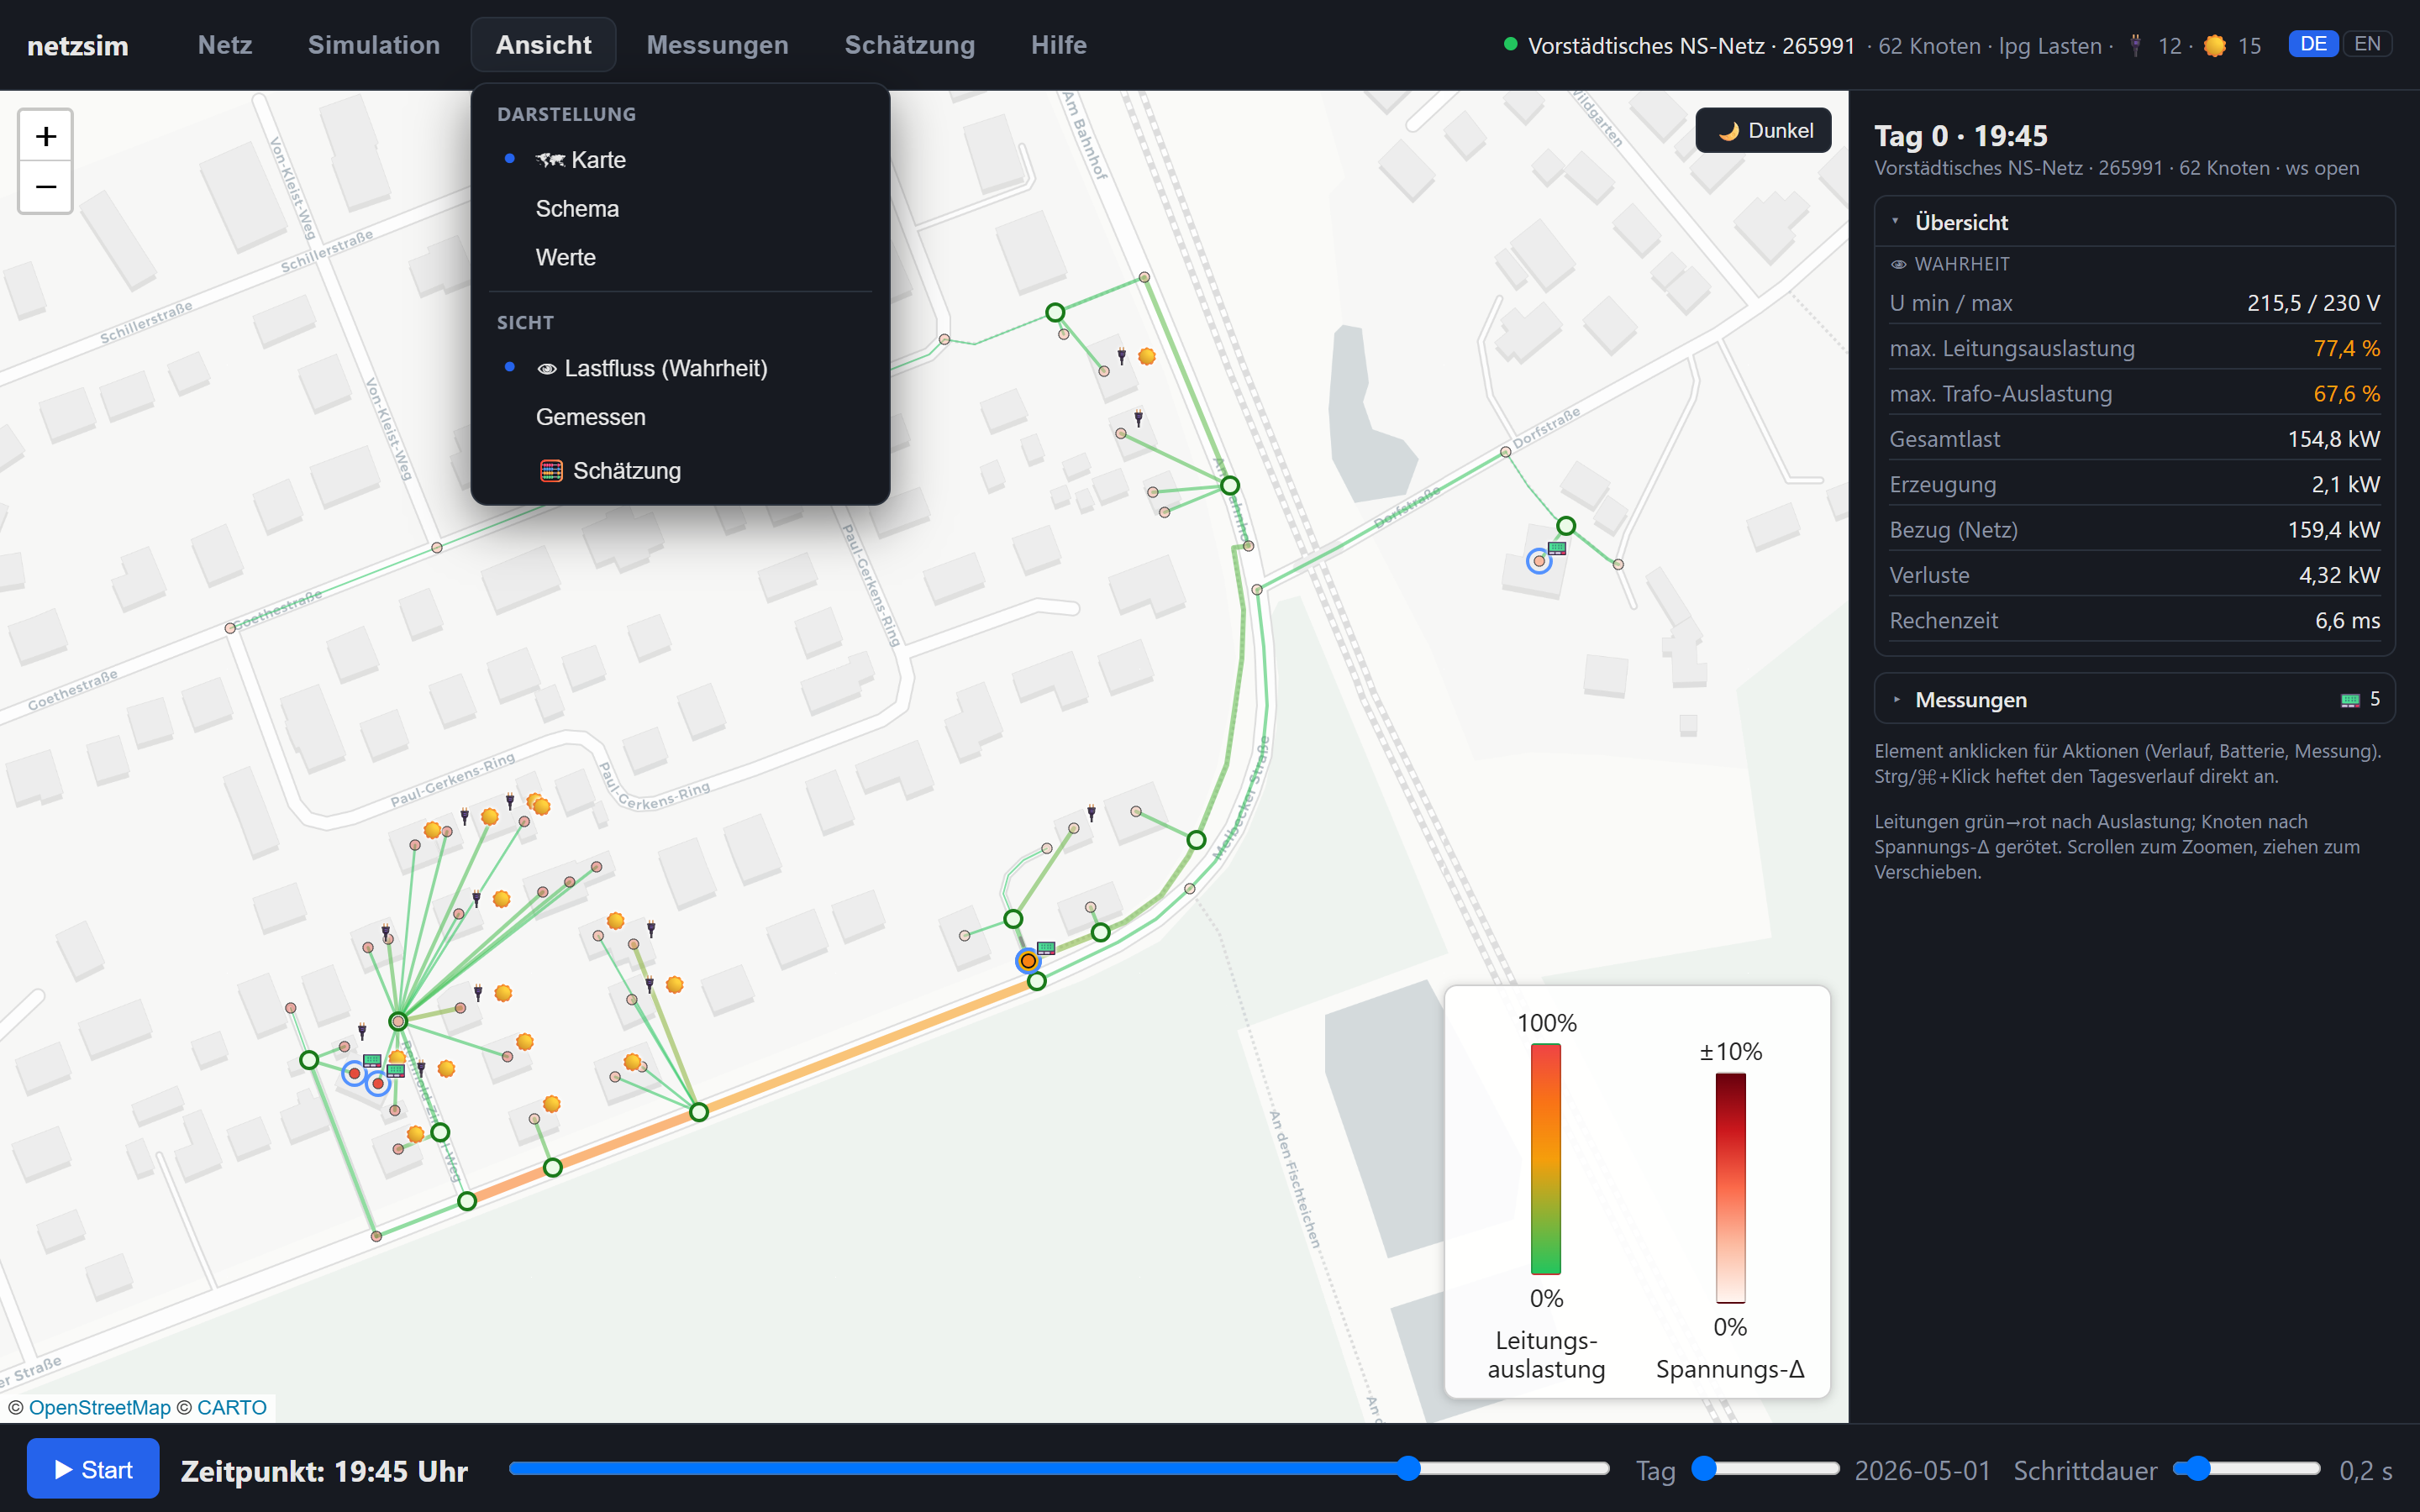
\includegraphics[width=\textwidth]{ui-menue}
  \caption{Die Menüleiste über der Live-Ansicht mit geöffnetem
    \ui{Datei}-Menü (kurze Befehlsliste, Listen als Untermenüs) und
    dem stets sichtbaren Sicht-Umschalter rechts daneben. Die
    Transportleiste (Start/Pause, Zeit, Tag, Schrittdauer) bleibt
    permanent am unteren Rand.}
  \label{fig:menue}
\end{figure}

Der typische Arbeitsablauf bleibt ein Dreischritt --- Netz wählen,
Lasten erzeugen, live beobachten. Die ersten beiden Schritte leben
in \emph{einer} Ansicht (\ui{Netz \& Lasten}), die in drei Spalten
von links nach rechts durchlaufen wird: \ui{1~·~Netz wählen},
\ui{2~·~Lasten \& Erzeugung}, \ui{3~·~Prüfen \& starten}. Alle
Beispiele dieses Kapitels stammen aus \emph{einem} durchgängigen
Arbeitsgang mit demselben Netz, sodass sich die Zahlen von Schritt
zu Schritt wiederfinden lassen.

\section{Schritt 1: Netz wählen oder importieren}

\ui{Datei} $\rightarrow$ \ui{Netz \& Lasten…} öffnet die kombinierte
Ansicht (auch der Klick auf den Netz-Chip rechts oben führt
hierher). Die linke Spalte listet alle verfügbaren Netze:

\begin{description}
  \item[\ui{Bibliothek}] mitgelieferte synthetische deutsche
    Verteilnetze (ding0) auf realer Geographie: Die Topologien
    sind künstlich, aber nach den Regeln realer Netzplanung
    erzeugt und an echten Orten verankert, sodass die Karte echte
    Straßen zeigt. Ausgeliefert werden die beiden Netze der
    Referenzszenarien (Kapitel~\ref{ch:scenarios}): ein
    \emph{ländliches} NS-Netz (reines Strahlennetz mit langem
    Ausläufer --- spannungskritisch) und ein \emph{vorstädtisches}
    NS-Netz (mehrere Stränge --- auslastungskritisch bei hoher
    Gleichzeitigkeit).\footnote{Die volle Bibliothek mit 20 Netzen
    (MS-Bezirke, städtische Netze, weitere Größen) lässt sich
    wiederherstellen, indem \texttt{data/grid\_library\_full.json}
    über \texttt{data/grid\_library.json} kopiert wird. Ein
    MS-Bibliotheksnetz lädt dann automatisch die straßengerouteten
    NS-Ortsnetze seines Bezirks mit; NS-Ortsnetze ohne Straßenmodell
    bleiben als \emph{Summenlast} an ihrer Station, und auf der
    Live-Karte filtert der Ebenenumschalter \ui{MS}/\ui{NS}/\ui{Alle}.}
  \item[\ui{Eigene Netze}] alle mit dem Editor \emph{gridedit}
    gezeichneten und exportierten Netze
    (Kapitel~\ref{ch:gridedit}).
  \item[\ui{Netz importieren…}] lädt eine Netzdatei (JSON aus
    gridedit oder gridgen) direkt in den Katalog. Die Datei wird
    beim Import probeweise konvertiert --- was sich nicht laden
    lässt, wird mit einer Fehlermeldung abgewiesen.
\end{description}

Nach der Auswahl erscheinen in der Mittelspalte die Kenndaten
(Knoten, Leitungen, Lasten, Trafo-Nennleistung) und rechts oben die
\emph{Struktur} des Netzes: eine dunkle Karte ohne Kartenhintergrund
--- blaue Kabel entlang der realen Straßenzüge, die Ortsnetzstation
bernsteinfarben, Kabelverteiler als grüne Quadrate, Hausanschlüsse
als grüne Punkte (Abbildung~\ref{fig:netz}).

\begin{figure}[htbp]
  \centering
  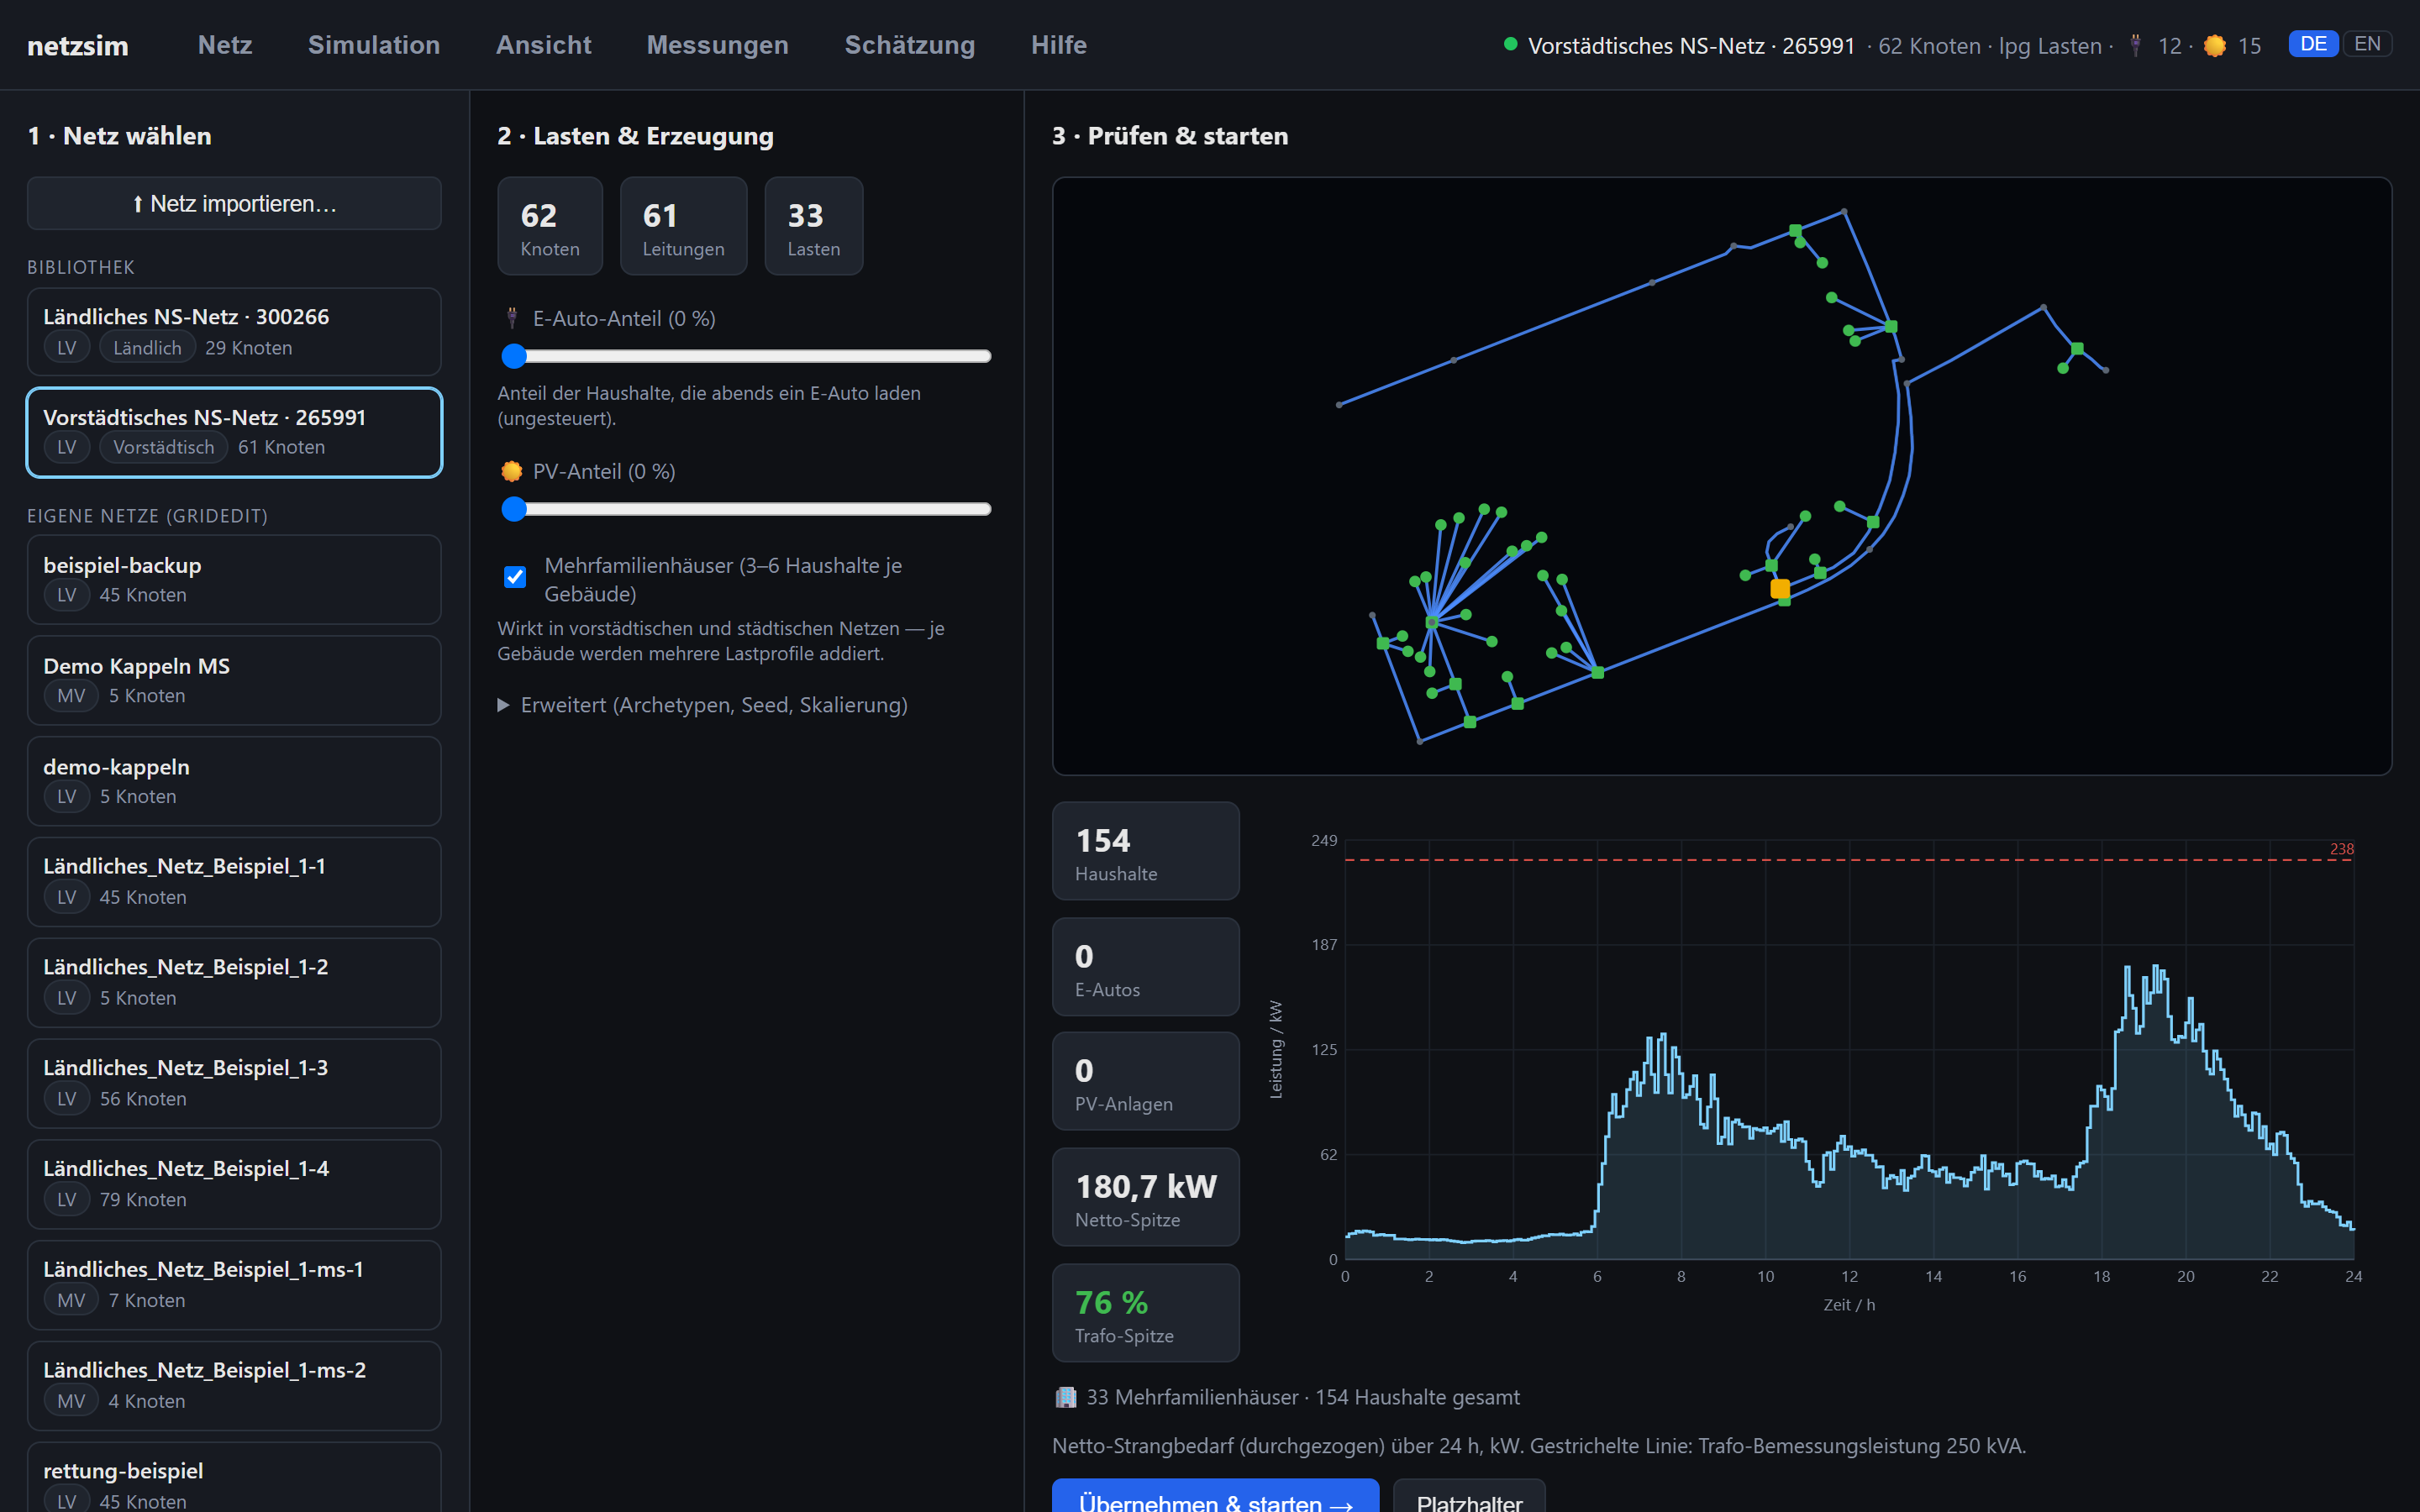
\includegraphics[width=\textwidth]{ui-netz}
  \caption{Die Ansicht \ui{Netz \& Lasten}: links Bibliothek, eigene
    Netze und der Datei-Import, in der Mitte die Kenndaten und
    Lastregler, rechts die Struktur des gewählten Netzes und die
    laufend aktualisierte Vorschau.}
  \label{fig:netz}
\end{figure}

\begin{beispiel}[Das Netz der folgenden Kapitel]
Die Wahl fällt auf das \emph{Vorstädtische NS-Netz~·~265991}:
62~Knoten, 61~Leitungen, 1~Ortsnetztransformator (250~kVA),
33~Hausanschlüsse an drei Strängen. Die Importhinweise melden
u.\,a., auf welche Standardgröße der Transformator dimensioniert
wurde. Ein Ortsteil dieser Größe ist ideal, um Spannungsband und
Leitungsauslastung gleichzeitig zu beobachten.
\end{beispiel}

\section{Schritt 2: Lasten erzeugen}

In der Mittelspalte \ui{2~·~Lasten \& Erzeugung} werden den
33~Gebäuden realistische Tagesprofile zugewiesen. Grundlage sind
Profile aus dem LoadProfileGenerator (LPG), der das Verhalten
konkreter Haushalte minutengenau simuliert --- Kochen,
Waschmaschine, Fernseher, Anwesenheit. Die Bibliothek enthält
u.\,a.\ folgende Archetypen (Jahresverbräuche der hinterlegten
Profile):

\begin{center}
\begin{tabular}{@{}llr@{}}
\toprule
Archetyp & Beschreibung & Jahresverbrauch \\
\midrule
CHR01 & Paar, beide berufstätig & 3\,776 kWh \\
CHR03 & Familie, 1 Kind, beide berufstätig & 4\,540 kWh \\
CHR05 & Familie, 3 Kinder, beide berufstätig & 5\,562 kWh \\
CHR07 & Single, berufstätig & 2\,248 kWh \\
CHR16 & Paar über 65 Jahre & 3\,842 kWh \\
CHR22 & Alleinerziehende, 1 Kind, berufstätig & 1\,620 kWh \\
CHR30 & Alleinstehender Rentner & 2\,142 kWh \\
CHR52 & Studenten-WG & 3\,161 kWh \\
\bottomrule
\end{tabular}
\end{center}

Einstellmöglichkeiten:

\begin{itemize}[nosep]
  \item \ui{E-Auto-Anteil} und \ui{Wallbox-Leistung} (3{,}7 / 11 /
    22~kW oder \ui{Zufall}: jede Wallbox bekommt zufällig eine der
    drei Größen --- dieselben Gebäude, nur gemischte Leistungen):
    der gewählte Anteil der Gebäude lädt abends \emph{ungesteuert}
    --- die Ladefenster streuen um den Feierabend, genau das
    erzeugt die kritische Gleichzeitigkeit.
  \item \ui{PV-Anteil} und \ui{PV-Größe pro Haushalt} (kWp):
    Dach-Photovoltaik als Einspeisung mit Schönwetter-Tagesgang.
    Die \ui{PV-Auslegung} wählt zwischen \ui{Gleiche Leistung} und
    \ui{Zufällige Leistung und Verteilung} --- dann streuen
    Anlagengröße (0{,}5--1{,}5-fach des Reglers) und Dachausrichtung
    (der Mittagspeak verschiebt sich je Anlage um bis zu
    $\pm$1{,}5~h) über die Anlagen.
  \item \ui{Mehrfamilienhäuser}: In vorstädtischen und städtischen
    Netzen hängt ein Hausanschluss selten an nur \emph{einem}
    Haushalt. Mit diesem Haken (Vorgabe: an) werden je Gebäude
    3--6 Haushaltsprofile \emph{addiert} --- die Lastsituation wird
    dadurch deutlich realistischer, denn die Gleichzeitigkeit
    innerhalb eines Gebäudes ist eine andere als zwischen
    Einfamilienhäusern. Die Zustandsschätzung
    (Kapitel~\ref{ch:observability}) kennt die Zählpunktzahl je
    Gebäude und skaliert ihre SLP-Annahme entsprechend.
  \item Unter \ui{Erweitert}: die Archetyp-Auswahl, der
    \ui{Zuweisungsmodus} (\ui{Reihum} verteilt die Archetypen der
    Reihe nach; \ui{Zufällig} würfelt --- derselbe \ui{Zufalls-Seed}
    erzeugt immer dieselbe Verteilung, alle Übungsgruppen mit
    Seed~0 sehen exakt dasselbe Netz), der \ui{Skalierungsfaktor}
    (mit 2{,}0$\times$ lässt sich ein Netz gezielt an seine Grenzen
    bringen) und der \ui{Leistungsfaktor} ($\cos\varphi$,
    Vorgabe~0{,}95) für die Blindleistung.
\end{itemize}

Die rechte Spalte \ui{3~·~Prüfen \& starten} rechnet bei jeder
Änderung automatisch nach --- in \emph{Scheinleistung} (kVA, über
den Leistungsfaktor aus der Wirklast gerechnet), damit alles direkt
mit der Nennleistung der Ortsnetzstation vergleichbar ist:
durchgezogen der Netto-Bedarf über 24~Stunden, gestrichelt die
Bruttolast vor PV, dazu als rote gestrichelte Linie die
\emph{Trafo-Bemessungsleistung}. Die Kennzahl \ui{max.\
Trafo-Auslastung} setzt die \ui{Leistungsspitze} des Tages (Bezug
\emph{oder} Rückspeisung) ins Verhältnis zur Nennleistung und färbt
sich ab 80\,\% gelb, ab 100\,\% rot --- so ist \emph{vor} dem Start
sichtbar, ob die Station die gewählte Lastsituation überhaupt trägt
(Abbildung~\ref{fig:lasten}).
\ui{Übernehmen \& starten} lädt das Netz mit den erzeugten Profilen
in die Live-Simulation. Alternativ lässt sich der Schritt mit
\ui{Platzhalter}-Lasten überspringen (glatte synthetische
Tageskurven --- ausreichend für Topologie-Demos, aber ohne das
realistische Zappeln echter Haushalte).

\begin{figure}[htbp]
  \centering
  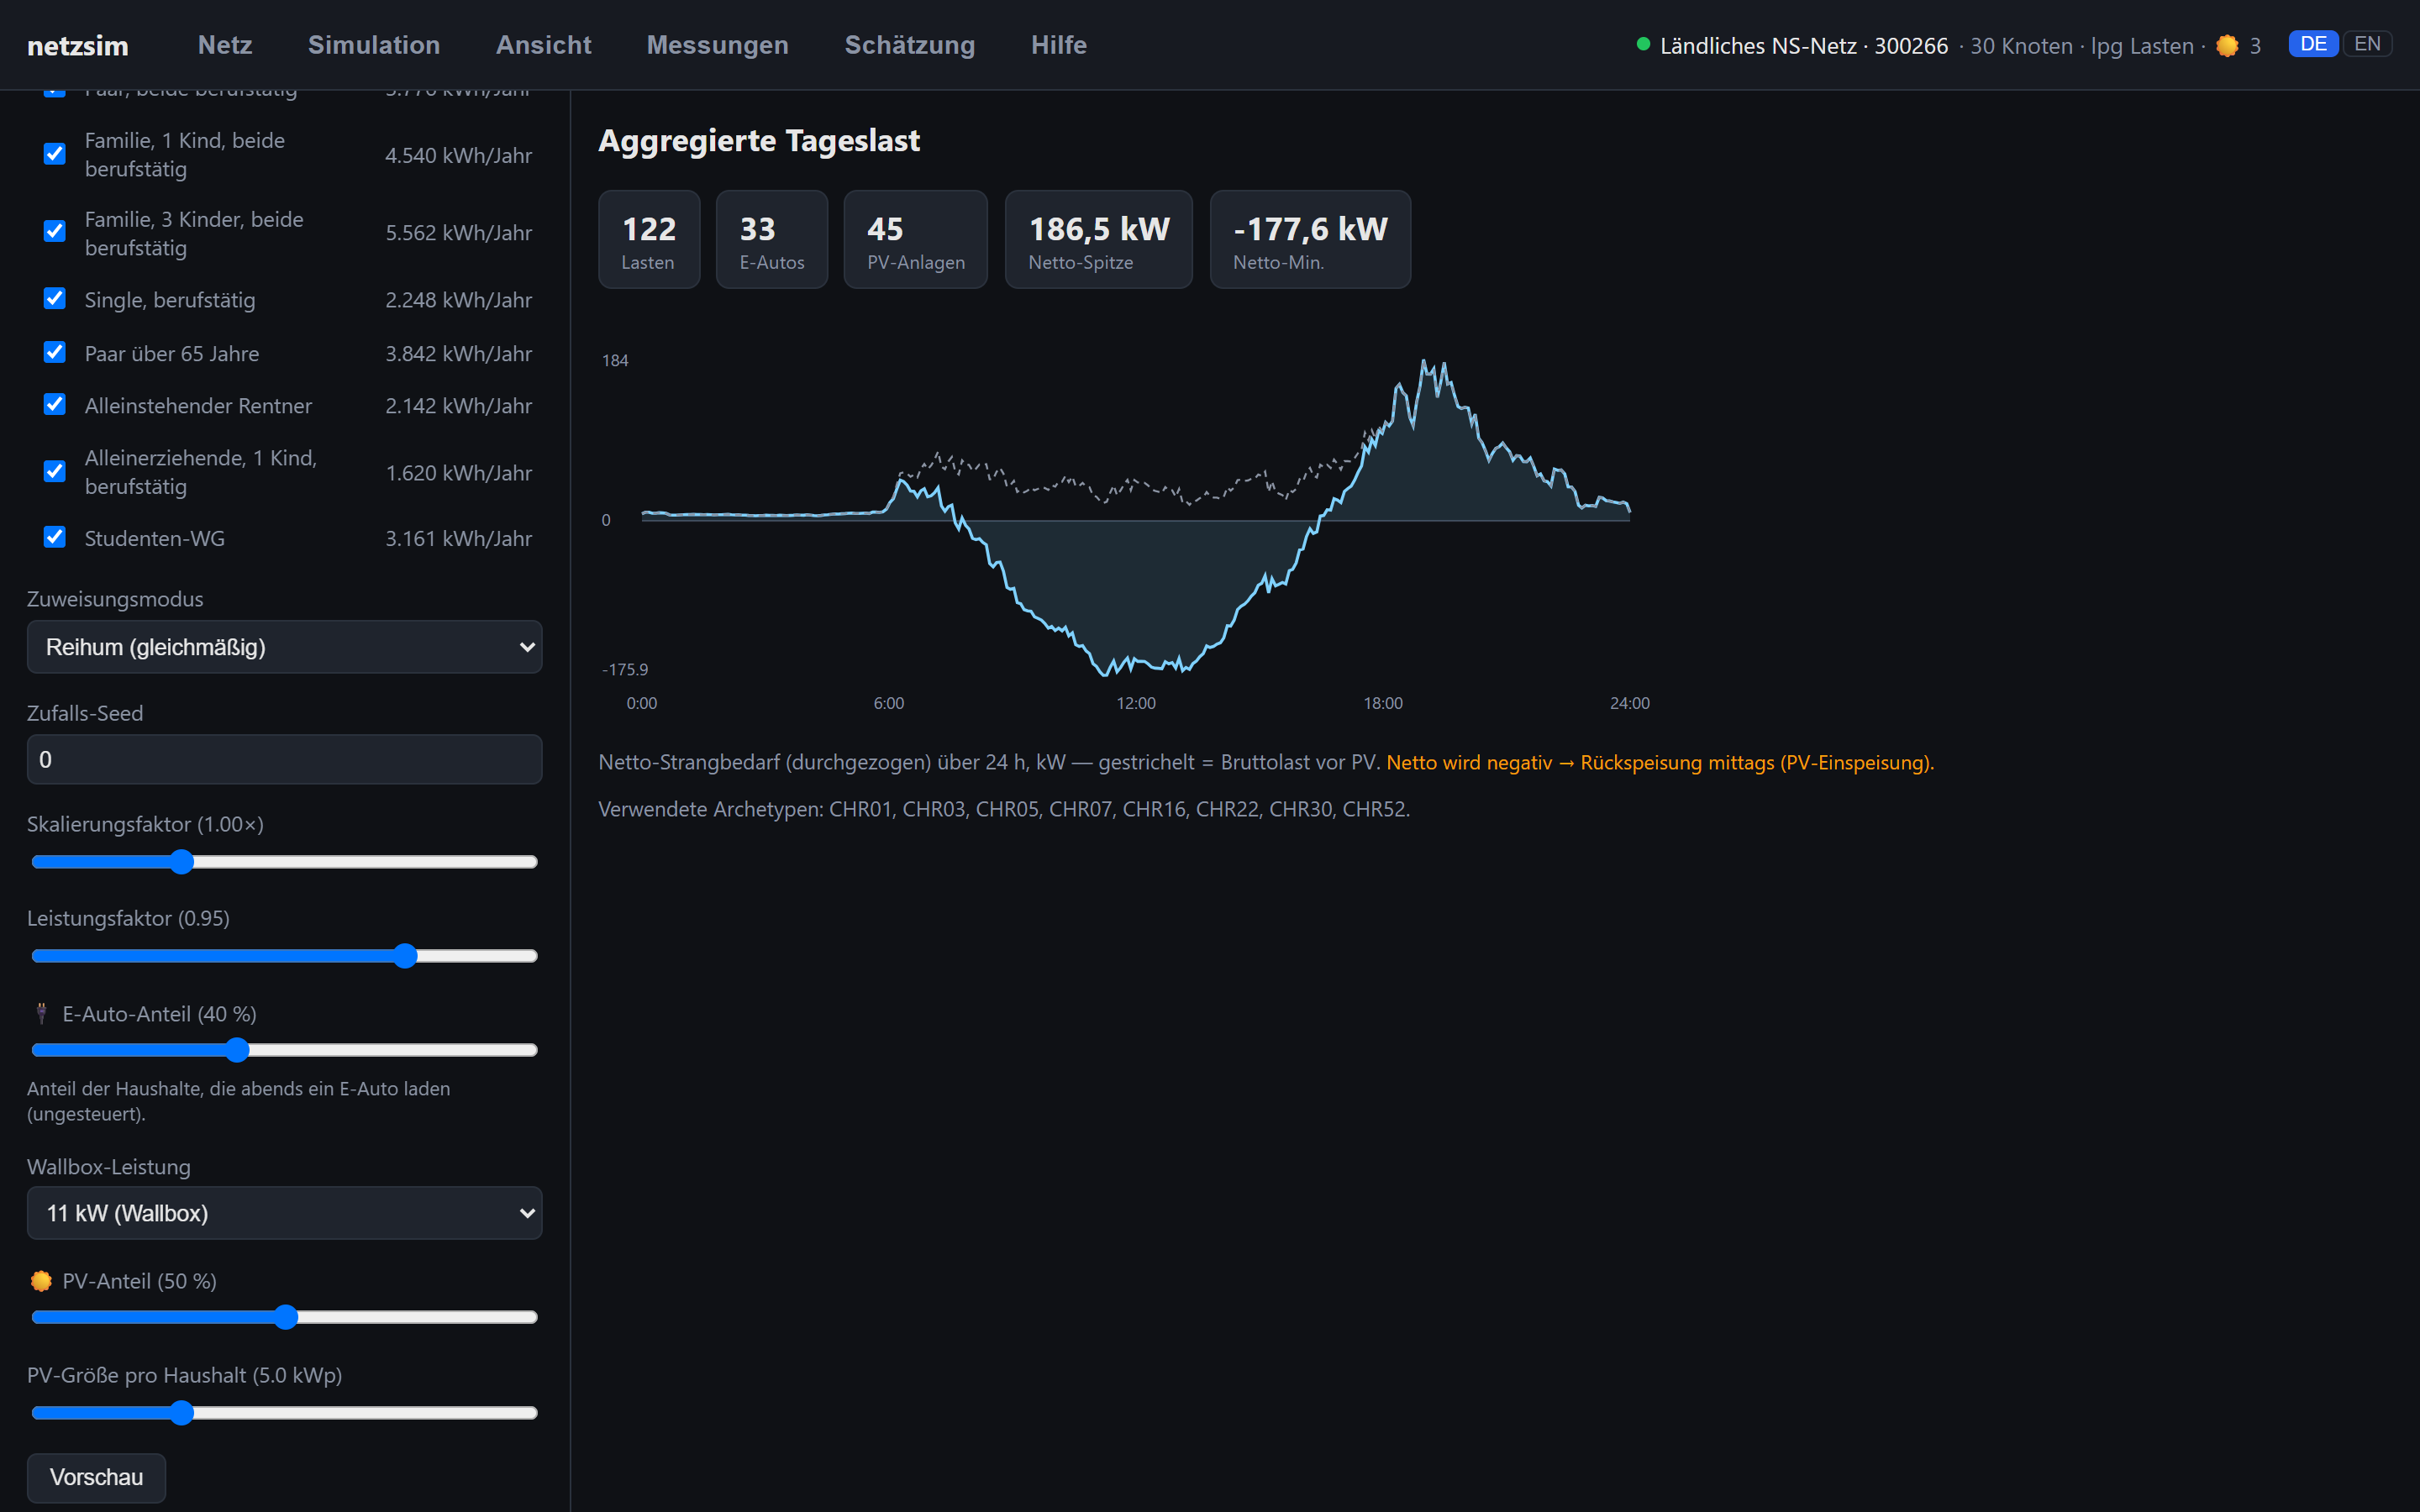
\includegraphics[width=\textwidth]{ui-lasten}
  \caption{Lasten \& Erzeugung mit Vorschau (hier 40\,\%
    E-Auto-Anteil, 50\,\% PV, Mehrfamilienhäuser aktiv): die
    Netto-Kurve wird mittags negativ --- der Strang speist zurück
    ---, die Abendspitze nähert sich der gestrichelten
    Trafo-Bemessungslinie, die Kennzahl \ui{max.\ Trafo-Auslastung}
    steht auf 92\,\%.}
  \label{fig:lasten}
\end{figure}

\begin{beispiel}[Gleichzeitigkeit, Mehrfamilienhäuser, E-Autos und PV]
Für das 33-Gebäude-Netz zeigt die Vorschau nacheinander:
\begin{itemize}[nosep]
  \item \textbf{Nur Haushalte:} Aus 33~Gebäuden werden mit dem
    Mehrfamilienhaus-Haken \textbf{154~Haushalte}; die
    \ui{Leistungsspitze} liegt bei \textbf{190~kVA} gegen 19:20 Uhr
    (\ui{max.\ Trafo-Auslastung} 76\,\%). Ohne den Haken (33
    Einzelhaushalte) wären es nur 60~kVA --- die Summe wächst aber
    \emph{nicht} linear mit der Haushaltszahl: nie kochen alle
    gleichzeitig. Diese \emph{Durchmischung} ist der Grund, warum
    eine 250-kVA-Station für einen ganzen Ortsteil reicht.
  \item \textbf{+ 40\,\% E-Autos (11~kW):} 12 Wallboxen laden abends
    ungesteuert. Die Spitze steigt auf \textbf{230~kVA}
    (+21\,\%), obwohl rechnerisch $12 \times 11 = 132$~kW
    installiert sind --- die Ladefenster überlappen nur teilweise.
    Die \ui{max.\ Trafo-Auslastung} springt auf \textbf{92\,\%} und
    färbt sich gelb: E-Mobilität wirkt fast ausschließlich auf die
    Abendspitze.
  \item \textbf{+ 50\,\% PV (5~kWp):} 15 Anlagen mit zusammen
    75~kWp drücken die Netto-Kurve mittags auf \textbf{$-$27~kVA}
    --- der Strang speist zurück. Die Abendspitze bleibt bei
    230~kVA: Abendspitze und Mittagstal liegen zeitlich so weit
    auseinander, dass PV die E-Auto-Spitze \emph{nicht} entlastet.
\end{itemize}
Genau dieses Auseinanderfallen von Erzeugung und Verbrauch motiviert
die Batteriespeicher aus Kapitel~\ref{ch:der}.
\end{beispiel}

Bei zusammengeschalteten MS+NS-Gebieten und bei MS-Netzen erhalten
nur echte Haushalte LPG-Profile --- Summenlasten und Großverbraucher
behalten ihre synthetischen Kurven.

\section{Schritt 3: Live-Ansicht}
\label{sec:live}

Die Seite \ui{Live} zeigt die laufende Simulation
(Abbildung~\ref{fig:live}).

\begin{figure}[htbp]
  \centering
  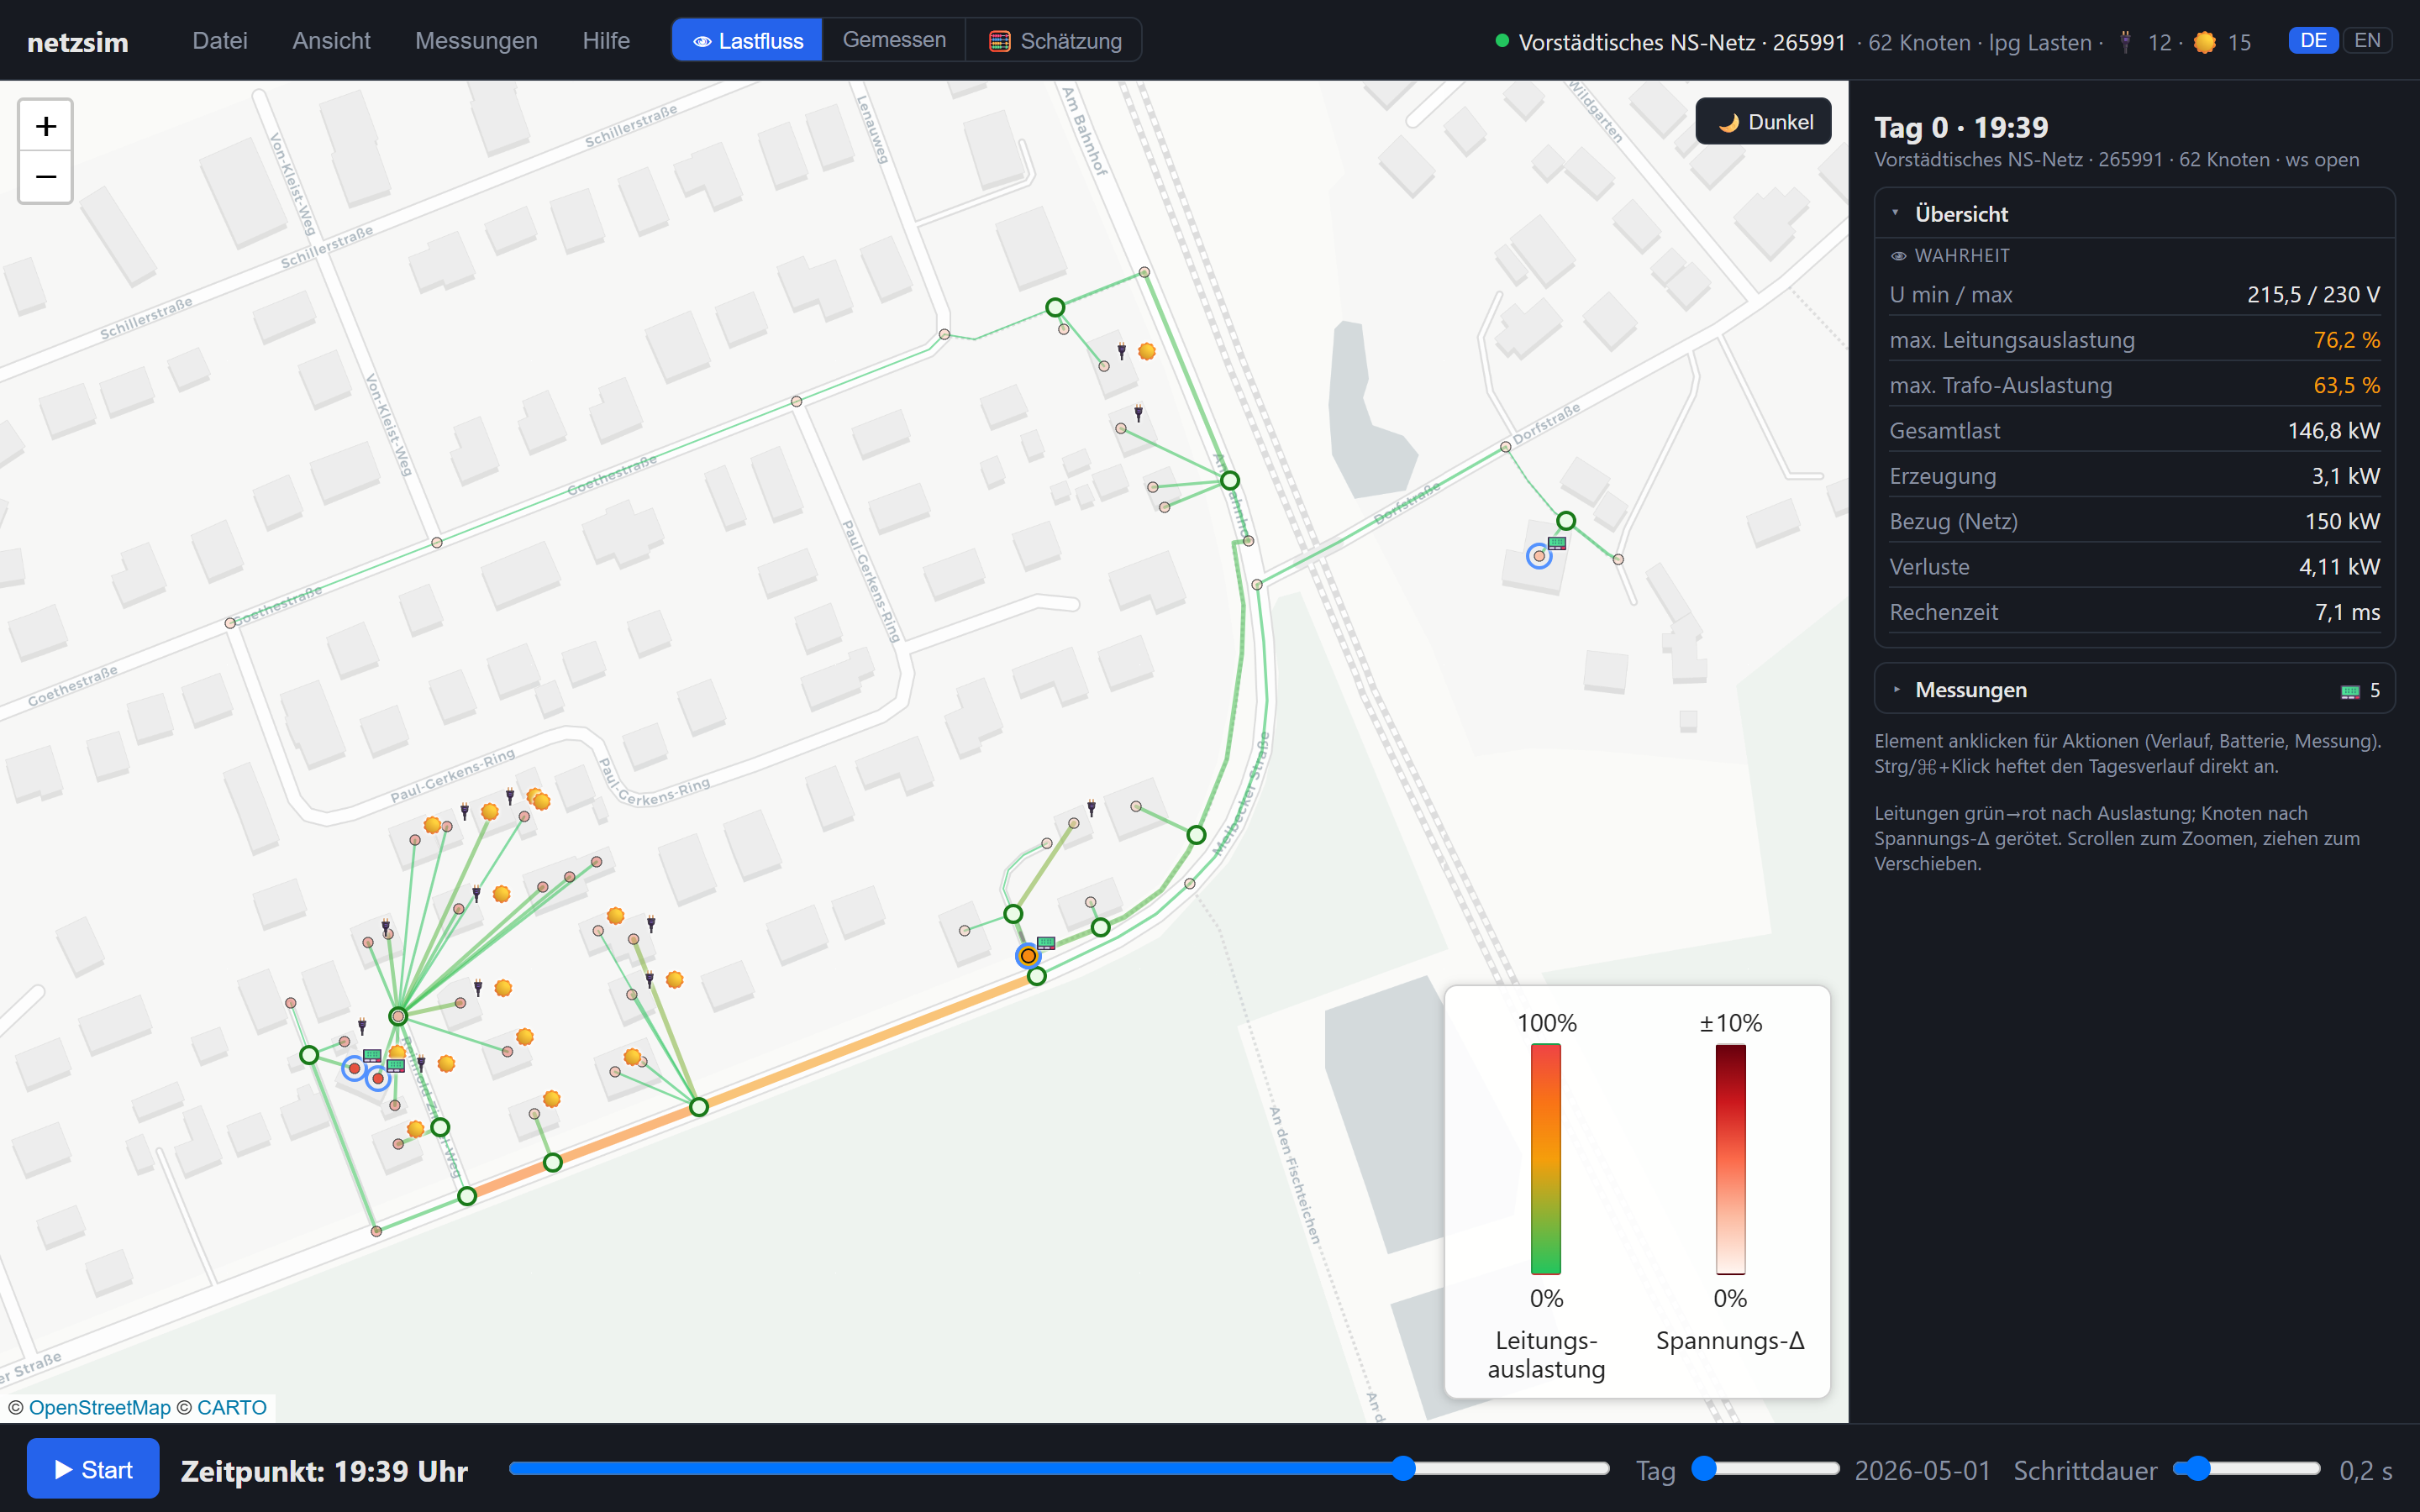
\includegraphics[width=\textwidth]{ui-live}
  \caption{Schritt 3 --- \ui{Live} zur Abendspitze (19:39 Uhr): Kabel
    färben sich nach Auslastung (hier bis 76\,\%), an den Häusern
    zeigen Symbole E-Auto-Ladungen und PV-Anlagen; rechts die
    Übersicht, unten Zeit-, Tag- und Schrittdauer-Regler.}
  \label{fig:live}
\end{figure}

\subsection{Darstellungen}

Die Darstellung wird im Menü \ui{Ansicht} gewählt:

\begin{description}
  \item[\ui{Karte}] Echte OpenStreetMap-Karte an den Koordinaten des
    Netzes (Hell/Dunkel umschaltbar). Leitungen färben sich
    grün~$\rightarrow$~gelb~$\rightarrow$~rot nach Auslastung ---
    bewusst ohne Blau: eine unbelastete Leitung ist \emph{gesund},
    nicht \glqq kalt\grqq. Knoten röten sich mit wachsender
    Spannungsabweichung; zwei Farbskalen am Kartenrand liefern die
    Zuordnung. Kabel folgen dem realen Straßenverlauf,
    Kabelverteiler erscheinen als grüne Kreise, Ortsnetzstationen
    bernsteinfarben.
  \item[\ui{Schema}] Schematische Netzdarstellung ohne Karte; die
    Leitungsbreite ist proportional zum Strom --- gut, um
    Lastpfade zu verfolgen.
  \item[\ui{Werte}] Blendet Live-Zahlenwerte direkt an Leitungen und
    Knoten ein (SCADA-Stil) --- für kleine Netze und Beamer-Demos.
\end{description}

\subsection{Steuerung}

\begin{itemize}[nosep]
  \item \ui{Start} / \ui{Pause} (Transportleiste unten) halten die
    Simulation an und setzen sie fort --- praktisch, um einen
    Zustand in Ruhe zu besprechen.
  \item Der \ui{Zeitpunkt}-Regler springt an eine beliebige Uhrzeit
    des Tages (siehe Beispiel in Abschnitt~\ref{sec:zeitmodell}).
  \item \ui{Schrittdauer} stellt die Realzeit pro Simulationsschritt
    ein --- 0{,}1~s zum schnellen Überfliegen eines Tages, 1--2~s
    zum Mitlesen der Werte.
  \item Der \ui{Tag}-Regler erscheint, wenn reale PV-Messtage geladen
    sind (Kapitel~\ref{ch:realpv}): jeder Tag legt eine andere
    gemessene Solarkurve auf die PV-Anlagen.
\end{itemize}

\subsection{Die Übersicht lesen}

Das Seitenpanel fasst den Netzzustand jedes Schrittes zusammen.
Anhand des Screenshots (19:39 Uhr, Abendspitze mit E-Autos):

\begin{center}
\small
\begin{tabular}{@{}lrl@{}}
\toprule
Kennzahl & Wert & Interpretation \\
\midrule
U min / max & 215{,}5 / 230 V & Tiefpunkt am Strangende: $-6{,}3\,\%$ \\
 & & (EN-50160-Band: $\pm 10\,\% \Rightarrow$ 207--253 V) \\
max.\ Leitungsauslastung & 76{,}2 \% & höchstbelastetes Kabel, noch Reserve \\
max.\ Trafo-Auslastung & 63{,}5 \% & 250-kVA-Station gut ausgelastet \\
Gesamtlast & 146{,}8 kW & Haushalte + ladende E-Autos \\
Erzeugung & 3{,}1 kW & Rest-PV der Abendsonne \\
Bezug (Netz) & 150 kW & Import aus dem MS-Netz \\
Verluste & 4{,}11 kW & $\approx 2{,}8\,\%$ der Last --- Abendspitze \\
 & & treibt die $I^2R$-Verluste \\
Rechenzeit & 7{,}1 ms & Lastfluss-Dauer dieses Schrittes \\
\bottomrule
\end{tabular}
\end{center}

Konvergiert ein Schritt nicht, vermerkt es die Kopfzeile; die
Simulation läuft mit dem nächsten Schritt normal weiter.

\begin{beispiel}[Was man um 19:39 Uhr auf der Karte sieht]
Der Hauptstrang von der Station zum dichtesten Ortsteil ist orange
(76\,\%), seine Ausläufer gelbgrün; an einem Dutzend Häusern
stecken E-Auto-Symbole. Fährt man mit der Maus über das orange
Kabel, zeigt der Tooltip Auslastung, Strom in Ampere und Wirkleistung.
Zwei Stunden später (Regler auf 21:30) sind die meisten Ladungen
beendet, das Netz wird wieder grün --- der gesamte Spannungstrichter
entspannt sich sichtbar von außen nach innen.
\end{beispiel}

\subsection{Interaktion mit Netzelementen}

Ein Klick auf einen Knoten, eine Leitung oder einen Transformator
öffnet ein Aktionsmenü:

\begin{itemize}[nosep]
  \item \ui{Tagesverlauf} heftet ein Diagramm des Elements als
    aufklappbare Sektion ins Seitenpanel;
    Strg/$\hat{}$\,+Klick heftet es direkt an. Je nach Elementtyp:
    \begin{itemize}[nosep]
      \item \emph{Knoten}: Leistung, aufgeschlüsselt nach
        Haushalt / E-Auto / PV (bei MS-Netzen auch Windkraft,
        Biogas), oder Spannung mit den EN-50160-Grenzen
        $\pm 10\,\%$ als rote Linien. Eine gelbe Marke zeigt die
        aktuelle Simulationszeit.
      \item \emph{Leitung}: Strom über den Tag gegen den Nennstrom
        (z.\,B. \glqq Nenn 225~A\grqq) --- Überlastphasen sind sofort
        sichtbar.
      \item \emph{Transformator}: Leistungsaustausch gegen die
        Nennleistung in beide Richtungen ($\pm$250~kVA) ---
        Rückspeisung erscheint als negativer Ast.
    \end{itemize}
    Die Tagesdiagramme folgen der gewählten \ui{Sicht}
    (Abschnitt~\ref{sec:sichten}): Im \ui{Lastfluss} zeigen sie die
    volle Wahrheit im Minutenraster, in \ui{Gemessen} nur die
    Messgrößen des Elements im Messraster, in der \ui{Schätzung}
    alle Ebenen überlagert. Angeheftete Elemente sind im Schema
    \emph{und} auf der Karte mit einem goldenen Ring markiert, damit
    die Diagramme im Seitenpanel eindeutig zuzuordnen sind.
  \item \ui{Messung platzieren} / \ui{entfernen} --- siehe
    Kapitel~\ref{ch:observability}.
  \item \ui{Batterie hinzufügen}, \ui{PV-Anlage hinzufügen},
    \ui{E-Auto-Ladung hinzufügen} --- siehe Kapitel~\ref{ch:der}.
  \item \ui{Regler platzieren} (an der Station: \ui{Netzregler}) ---
    die netzdienliche Steuerung gegen Überlast,
    Abschnitt~\ref{sec:controller}.
\end{itemize}

\begin{beispiel}
Strg+Klick auf das letzte Haus des langen Ausläufers, Modus
\ui{Spannung}: Die Kurve hängt tagsüber nahe 230~V, sackt aber
zwischen 18 und 21 Uhr Richtung 215~V ab --- deutlich sichtbar über
dem $-10\,\%$-Limit bei 207~V, aber der Trend pro zusätzlichem
E-Auto lässt sich hier unmittelbar demonstrieren: über das
Aktionsmenü desselben Knotens eine \ui{E-Auto-Ladung hinzufügen}
und die Kurve im angehefteten Diagramm neu bewerten.
\end{beispiel}

% ===================================================================
\chapter{Beobachtbarkeit und Zustandsschätzung}
\label{ch:observability}

\section{Grundidee}

Der Simulator berechnet in jedem Schritt den vollständigen Lastfluss
(die \emph{Wahrheit}). Sichtbar wird ein Messwert aber nur dort, wo
ein Messgerät platziert wurde. Das entspricht der Realität: In
deutschen Niederspannungsnetzen war historisch praktisch nichts
gemessen --- der Netzbetreiber kannte die Zählerstände fürs
Abrechnen, aber nicht den momentanen Netzzustand. Ohne Messungen
zeigt netzsim das Netz daher grau mit Fragezeichen: unbeobachtbar.

\section{Messgeräte platzieren}

Zwei Gerätetypen stehen zur Verfügung (per Klick auf ein Element,
über die Sektion \ui{Messungen} im Seitenpanel oder gesammelt über
das Menü \ui{Messungen}):

\begin{description}
  \item[Smart Meter (Knoten)] liefert die Spannung, Wirk- und
    Blindleistung des Knotens sowie den daraus abgeleiteten Strom
    ($I = S / (\sqrt{3} \cdot U_{LL})$; die Simulation rechnet
    symmetrisch, die Werte sind dreiphasige Summen).
  \item[Trafo-Messung] liefert Auslastung sowie P/Q/I der
    Oberspannungsseite des Transformators --- das Pendant zur
    digitalen Ortsnetzstation.
\end{description}

Leitungen tragen bewusst \emph{keine} Messung --- Leitungsströme
bleiben unbekannt, solange die Wahrheit ausgeblendet ist. Gerade das
höchstbelastete Kabel ist also unsichtbar, wenn dort niemand misst.

Schnell-Aktionen im Menü \ui{Messungen}: \ui{Alle Knoten},
\ui{Stationen} (nur Stations-Trafos), \ui{Alle Trafos}, \ui{Alle
löschen}. Die \ui{Abdeckung} (gemessene Knoten/Trafos) wird dort und
in der Übersicht laufend angezeigt (Abbildung~\ref{fig:beobachtet}).

\begin{figure}[htbp]
  \centering
  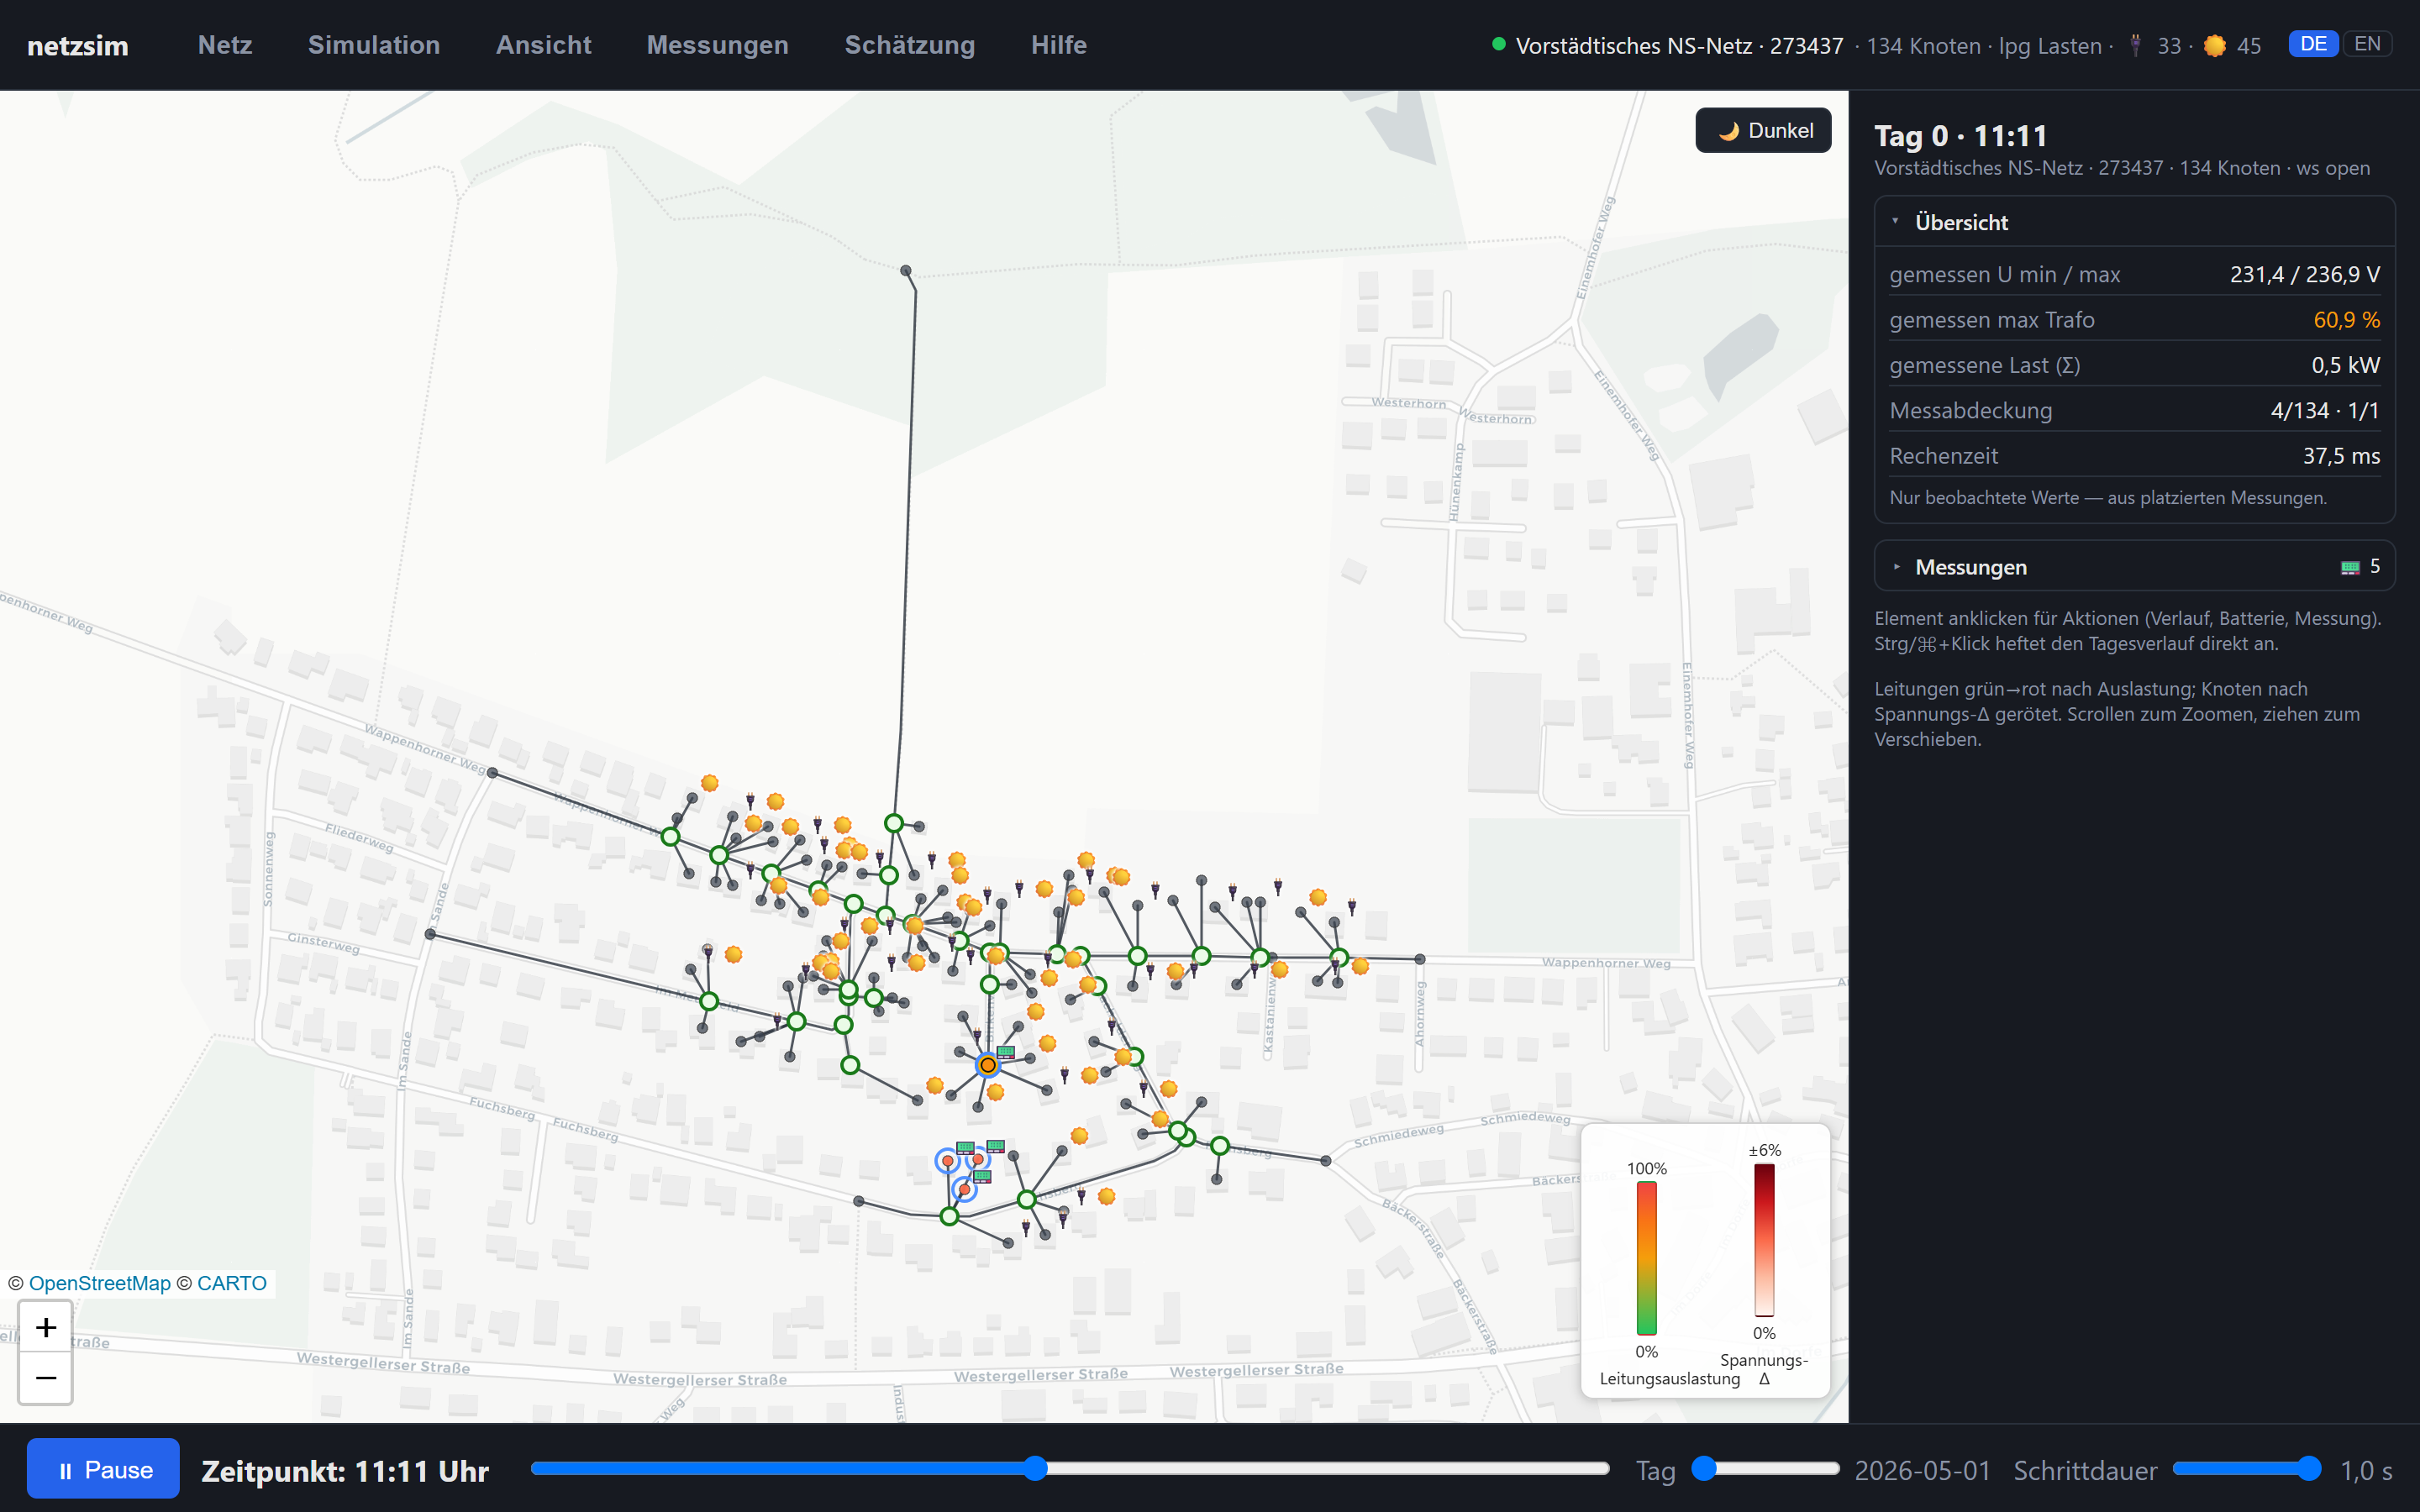
\includegraphics[width=\textwidth]{ui-beobachtet}
  \caption{Sicht \ui{Gemessen}: nur vier Knoten
    und der Stations-Trafo tragen Messungen --- alles andere ist grau
    und unbekannt. Die Übersicht zeigt ausschließlich gemessene
    Größen samt Messabdeckung (4/62 Knoten).}
  \label{fig:beobachtet}
\end{figure}

Zwei Mess-Modi bilden reale Smart-Meter-Tarifanwendungsfälle (TAF)
nach dem deutschen Messstellenbetriebsgesetz ab --- und zwar
\textbf{je Gerät}, so wie im echten Netz TAF-7-Haushaltszähler und
minütlich messende SMGWs an Anlagen und Wallboxen nebeneinander
existieren:

\begin{description}
  \item[TAF 9/10/14] \glqq Netzzustandsdaten\grqq: Spannung, P, Q und
    Strom im Minutentakt --- das, was sich ein Netzbetreiber wünscht.
  \item[TAF 7] \glqq Zählerstandsgang\grqq: nur der
    15-Minuten-Mittelwert der Wirkleistung --- das, was der
    Standard-Rollout tatsächlich liefert. Die Granularität ist
    strikt: Innerhalb eines Fensters ändert sich der Wert nie, und
    direkt nach dem Platzieren oder Umschalten liefert das Gerät
    \emph{gar nichts}, bis die erste Viertelstunde vollendet ist.
\end{description}

Umgeschaltet wird an zwei Stellen: Der kleine
\ui{TAF9/10/14}/\ui{TAF7}-Umschalter im Messwerte-Block einer
Element-Sektion stellt \emph{dieses eine Gerät} um; die beiden
Einträge im Menü \ui{Messungen} setzen \emph{alle} platzierten
Geräte auf einmal und bestimmen die Vorgabe für neue.

\begin{beispiel}[Warum TAF 7 Spitzen verschluckt]
Eine 22-kW-Wallbox lädt von 19:02 bis 19:12 Uhr --- zehn Minuten
volle Leistung. Ein TAF-9-Gerät zeigt diese 22~kW minutengenau. Ein
TAF-7-Zähler liefert für das Intervall 19:00--19:15 nur den
Mittelwert $22 \cdot \tfrac{10}{15} \approx 14{,}7$~kW --- ein
Drittel der Spitze ist \emph{in den Messdaten} verschwunden, im
Kabel aber natürlich geflossen. Der Umschalter im Messwerte-Block
des Hauses macht den Unterschied unmittelbar sichtbar; ein
realistisches Messkonzept mischt beide: die Nachbarschaft auf TAF~7,
nur die Wallbox mit einem 1-min-SMGW.
\end{beispiel}

\section{Die drei Ansichtsmodi}
\label{sec:sichten}

Der Sicht-Umschalter sitzt als dauerhaft sichtbares Segment rechts
neben den Menüs in der Menüleiste --- ein Klick genügt:

\begin{description}
  \item[\ui{Lastfluss (Wahrheit)}] Der echte Lastfluss wird
    vollständig eingeblendet --- die Vergleichs- und Lehransicht.
  \item[\ui{Gemessen}] Werte nur an platzierten
    Messungen, alles andere grau. Der Standardblick des Betreibers.
  \item[\ui{Schätzung}] Die WLS-Zustandsschätzung wird wie ein
    Lastfluss dargestellt (siehe unten).
\end{description}

Jede Sicht zeigt --- und lädt --- konsequent nur ihre eigene
Datenlage. Am deutlichsten wird das in den angehefteten
Tagesdiagrammen:

\begin{description}[nosep]
  \item[\ui{Lastfluss}] Alle Größen (Lasten an den Knoten, Ströme in
    den Leitungen, Trafo-Auslastung) liegen im vollen
    \textbf{1-Minuten-Raster} der Simulation vor; eine
    Zustandsschätzung wird hier gar nicht erst gerechnet, die
    Diagramme laden entsprechend schnell.
  \item[\ui{Gemessen}] Es erscheint ausschließlich, was das Messgerät
    des Elements wirklich liefert --- im Raster des gewählten
    Messmodus: \ui{TAF 9/10/14} minütlich mit Spannung, \ui{TAF 7}
    nur als \textbf{15-Minuten-Mittelwert der Wirkleistung}, ohne
    Spannung (die Kurve wird zur Treppenfunktion). Die gemessene
    Netz-Wirkleistung eines Knotens kann bei PV-Einspeisung negativ
    werden --- kein Messgerät kennt dagegen die Aufteilung in
    Haushalt/E-Auto/PV, sie wird hier bewusst nicht gezeigt. Knoten
    ohne Messung und sämtliche Leitungen zeigen statt eines
    Diagramms einen Hinweis: Leitungen tragen keine Messgeräte,
    ihre Ströme existieren nur im Lastfluss oder in der Schätzung.
  \item[\ui{Schätzung}] Die Diagramme überlagern alle drei Ebenen:
    die Wahrheitskurve, die Messwerte (fast-weiße \glqq
    Geräte\grqq-Kurve) und die Schätzkurve --- so ist unmittelbar
    sichtbar, wie nah die Schätzung an der Wahrheit liegt und
    welche Stützstellen sie dafür hatte.
\end{description}

\begin{beispiel}[Die Summe lügt nicht --- sie ist nur unvollständig]
Im Screenshot (Abbildung~\ref{fig:beobachtet}) meldet die Übersicht
\glqq gemessene Last ($\Sigma$) 12{,}9~kW\grqq{} --- die Wahrheit im
selben Moment: 146{,}8~kW. Die 12{,}9~kW sind schlicht die Summe der
vier gemessenen Hausanschlüsse. Wer nur auf Messwerte schaut, sieht
9\,\% des Geschehens; die \glqq gemessen max Trafo 63{,}5\,\%\grqq{}
der Stationsmessung ist dagegen belastbar, weil durch den Trafo
\emph{alles} fließt. Diese Asymmetrie --- Summenmessung top,
Ortsauflösung null --- ist der Kern des Beobachtbarkeitsproblems.
\end{beispiel}

Ist der Server im \emph{strikten Modus} konfiguriert
(\texttt{NETZSIM\_EXPOSE\_GROUND\_TRUTH=false}), verlässt die
Wahrheit den Server gar nicht erst: \api{/state}, \api{/ws} und
\api{/history} enthalten nur noch die Messwert-Projektion, der
Wahrheits-Umschalter verschwindet aus der Oberfläche. Damit lassen
sich Übungen abnahmesicher stellen (\glqq Schätzen Sie die Spannung
am Knoten~57\grqq), ohne dass die Lösung per API abgreifbar wäre.

\section{Zustandsschätzung}

Sobald mindestens eine Messung platziert ist, läuft parallel eine
WLS-Zu\-stands\-schät\-zung (weighted least squares) --- die Sicht des
Netzbetreibers. In die Schätzung fließen nur Dinge ein, die ein
Betreiber tatsächlich hat:

\begin{itemize}[nosep]
  \item das Netzmodell (Leitungen, Transformatoren mit Impedanzen),
  \item die Messwerte der platzierten Geräte samt Slack-Sollwert,
  \item strukturelles Wissen über Null-Einspeisungs-Knoten ---
    an Muffen und Kabelverteilern wird sicher nichts verbraucht,
  \item Pseudo-Messungen aus Standard-Lastannahmen: für jeden
    ungemessenen Hausanschluss das Tagesmittel seiner Lastklasse,
    mit bewusst großer Unsicherheit gewichtet.
\end{itemize}

Die Übersicht zeigt neben den geschätzten Kennzahlen den
\ui{Schätzfehler max $|\Delta U|$} gegen die Wahrheit.
Abbildung~\ref{fig:schaetzung} zeigt die Schätz-Ansicht mit nur fünf
Messgeräten.

Die Schätzung rechnet dabei im \emph{Messraster}: Sobald auch nur
ein Gerät im Modus \ui{TAF 9/10/14} minütlich neue Werte liefert,
wird minütlich neu geschätzt (die TAF-7-Geräte steuern dann eben nur
alle 15~Minuten frische Lastgangwerte bei). Sind dagegen
\emph{alle} Geräte auf \ui{TAF 7}, entsteht eine neue Schätzung nur
an den Viertelstundengrenzen --- dazwischen hält sie den letzten
Stand. Auf großen Netzen wird zusätzlich automatisch gedrosselt
(die Schätzung rechnet dann z.\,B. nur jeden dritten Schritt),
damit die Simulation flüssig bleibt.

\begin{figure}[htbp]
  \centering
  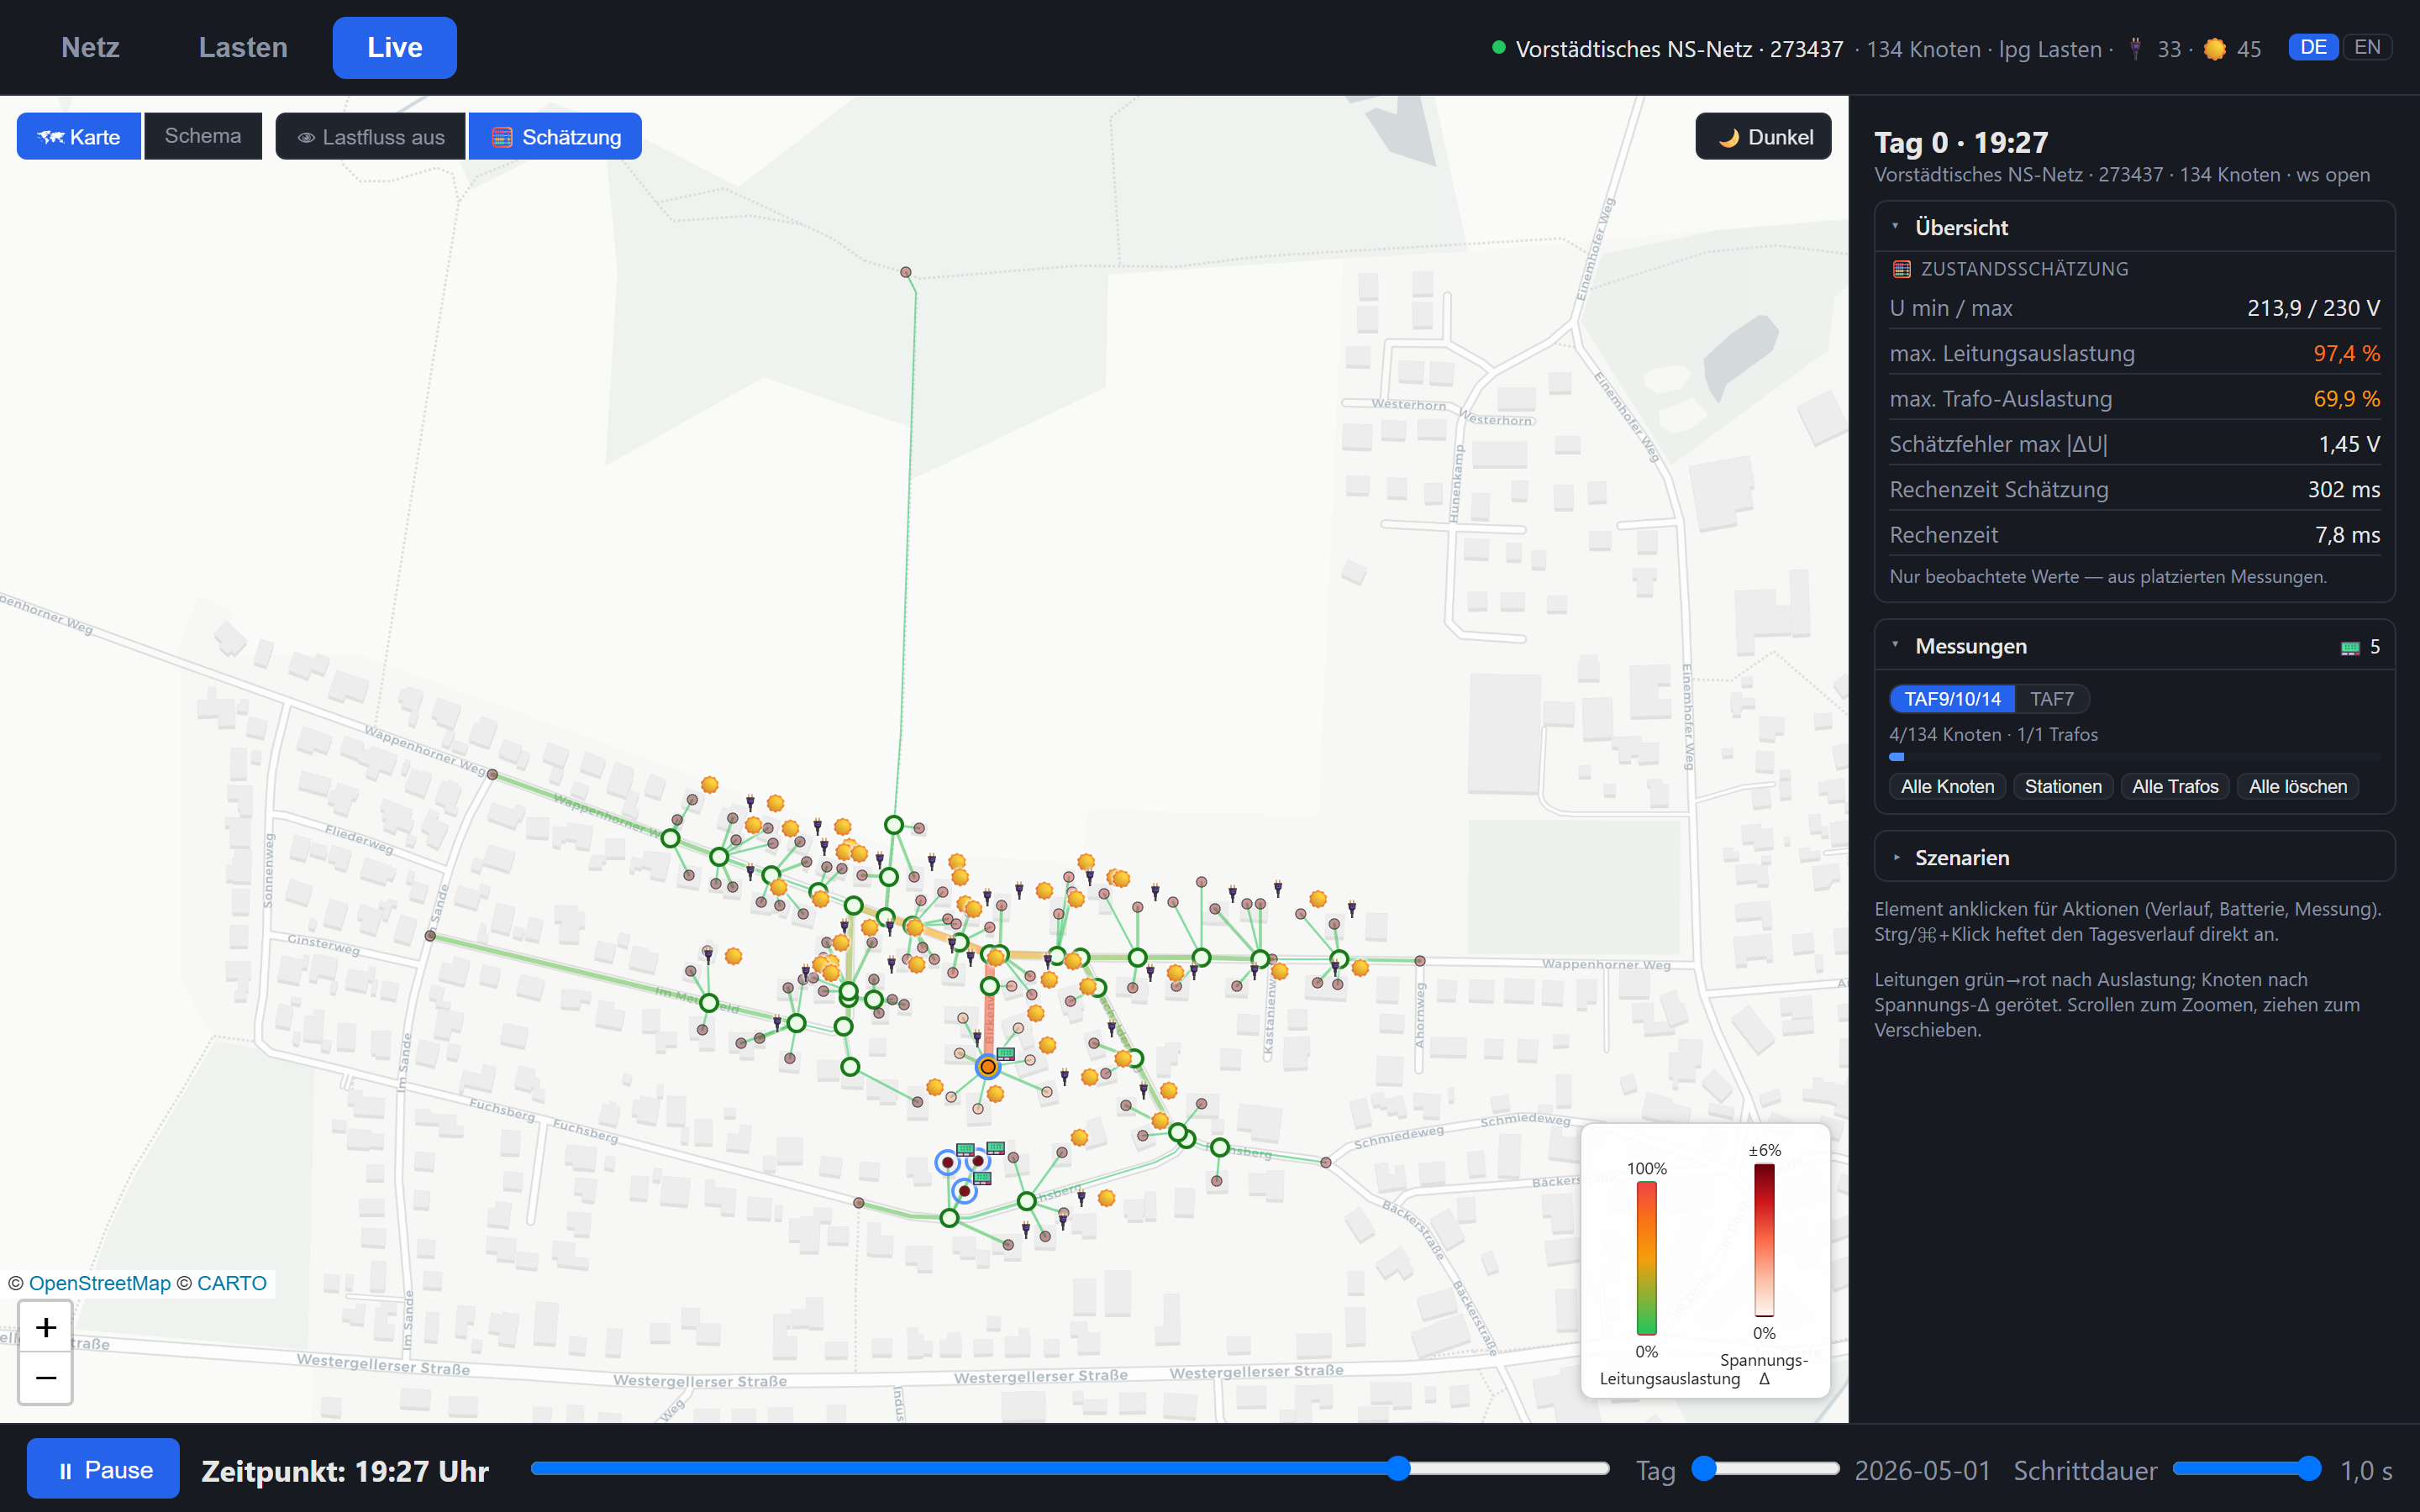
\includegraphics[width=\textwidth]{ui-schaetzung}
  \caption{Sicht \ui{Schätzung}: Aus fünf Messungen und dem
    Netzmodell rekonstruiert die WLS-Zustandsschätzung den kompletten
    Netzzustand --- die Karte färbt sich wieder, die Übersicht weist
    den Schätzfehler gegen die Wahrheit aus (hier 1{,}6~V; er
    konzentriert sich auf den Strang ohne Messung).}
  \label{fig:schaetzung}
\end{figure}

\begin{beispiel}[Messkampagne im Experiment]
Ein lohnender Unterrichtsverlauf auf dem 62-Knoten-Netz zur
Abendspitze (19:39 Uhr):
\begin{enumerate}[nosep]
  \item \textbf{Nur Stations-Trafo} (Preset \ui{Stationen}): Die
    Schätzung kennt die Gesamtbilanz und verteilt sie nach
    Standardannahmen. Zur Abendspitze passt das erstaunlich gut
    (max.\ Fehler \textbf{1{,}3~V}) --- Haushalte verhalten sich
    abends profilähnlich. Aber: \emph{Wo} der Fehler sitzt, weiß
    niemand.
  \item \textbf{+ 3 Smart Meter} in den belasteten Strängen
    (Screenshot): Die gemessenen Stränge werden fast exakt --- am
    kritischen Strangende schrumpft der Fehler von 0{,}5 auf
    0{,}1~V. Die Kennzahl \ui{max $|\Delta U|$} fällt trotzdem
    nicht (\textbf{1{,}6~V}): Der Restfehler ist in den einen
    Strang gewandert, in dem \emph{niemand} misst. Die eine Zahl
    sagt also nur, wie schlecht es an der blindesten Stelle steht.
  \item \textbf{Alle Knoten} (Preset): Der Fehler verschwindet
    praktisch ($< 0{,}1$~V) --- Vollausstattung macht die Schätzung
    exakt, kostet im echten Netz aber Millionen.
\end{enumerate}
Merksatz, den das Experiment liefert: \emph{Messungen wirken lokal.}
Der Fehler verschwindet dort, wo gemessen wird --- und sammelt sich
dort, wo niemand misst. Deshalb gehören Messungen an die kritischen
Stellen, nicht irgendwohin.
\end{beispiel}

% ===================================================================
\chapter{Anlagen und Regler: Batterien, PV, E-Autos, Steuerung}
\label{ch:der}

Alle Anlagen lassen sich zur Laufzeit über das Element-Menü eines
Knotens hinzufügen, umkonfigurieren und entfernen --- die Simulation
läuft dabei weiter, der Effekt ist im nächsten Schritt sichtbar.

\section{Batteriespeicher}

Eine Batterie wird an einem Knoten (oder an der NS-Sammelschiene des
Transformators) platziert; Kapazität (kWh) und Leistung (kW) sind
einstellbar. Drei Strategien stehen zur Wahl:

\begin{description}
  \item[\ui{Eigenverbrauch}] nimmt lokalen PV-Überschuss auf und
    deckt lokale Last --- die Heimspeicher-Logik.
  \item[\ui{Spitzenlastkappung}] entlädt bei Lastspitzen, lädt in
    Tälern --- die Netzbetreiber-Logik.
  \item[\ui{Preis}] lädt bei niedrigen, entlädt bei hohen
    Day-Ahead-Preisen (reale aWATTar-Stundenpreise, siehe
    Kapitel~\ref{ch:realpv}) --- die Händler-Logik.
\end{description}

Die Batterie-Sektion im Seitenpanel zeigt den Tagesverlauf von
Ladezustand (SOC) und Leistung; bei der Preis-Strategie zusätzlich
die Preiskurve mit markierten Kauf-/Verkaufsfenstern.

\begin{beispiel}[Dieselbe Batterie, drei Charaktere]
Eine 10-kWh-/5-kW-Batterie am PV-Haus mit 10~kWp:
\begin{itemize}[nosep]
  \item \emph{Eigenverbrauch}: lädt ab ~9 Uhr aus dem
    PV-Überschuss, ist gegen 14 Uhr voll (SOC 100\,\%), entlädt ab
    Sonnenuntergang in die Abendlast und ist gegen Mitternacht
    leer. Nebeneffekt am Netz: Die mittägliche Rückspeisespitze des
    Hauses sinkt um die Ladeleistung.
  \item \emph{Spitzenlastkappung} (besser an der NS-Sammelschiene
    der Station): wartet den Tag über, entlädt konzentriert
    zwischen 18 und 21 Uhr gegen die E-Auto-Spitze und holt sich
    die Energie nachts zurück --- die Trafo-Auslastungskurve wird
    oben \glqq abrasiert\grqq.
  \item \emph{Preis}: folgt der Börse statt der Physik --- lädt in
    den billigen Mittags- und Nachtstunden, verkauft in die teuren
    Abendstunden. Je nach Preistag deckt sich das mit der
    Netzentlastung --- oder eben nicht: ein schöner Anlass, über
    netzdienliche vs.\ marktdienliche Speicher zu diskutieren.
\end{itemize}
\end{beispiel}

\section{PV-Anlagen und E-Auto-Ladung}

\begin{itemize}[nosep]
  \item \ui{PV-Anlage hinzufügen} installiert Dach-PV am Knoten; die
    Größe (kWp) ist anschließend im Konfigurationsfeld der
    Knoten-Sektion einstellbar.
  \item \ui{E-Auto-Ladung hinzufügen} ergänzt eine Wallbox-Ladung;
    \ui{Beginn} und \ui{Dauer} (1--4~h) des Ladefensters sind
    verschiebbar.
\end{itemize}

\begin{beispiel}[Gesteuertes Laden von Hand]
Am langen Ausläufer des Beispielnetzes laden drei Nachbarn ab
18:00 Uhr gleichzeitig --- der Knoten fällt auf 217~V. Verschiebt
man die drei Ladefenster über die DER-Konfiguration auf 18:00,
20:00 und 22:00 Uhr (je 2~h), bleibt jede einzelne Ladung gleich
lang, aber die Spannung unterschreitet 224~V nicht mehr. Das ist
gesteuertes Laden (\S\,14a EnWG) im Kleinen --- ohne dass ein
einziger Kunde weniger Energie bekommt.
\end{beispiel}

\section{Überlast-Regler (netzdienliche Steuerung)}
\label{sec:controller}

Der Überlast-Regler ist das Werkzeug, um Abhilfe \emph{im} Netz zu
demonstrieren: eine netzdienliche Steuerung nach dem Vorbild von
\S\,14a~EnWG (Dimmen steuerbarer Verbrauchseinrichtungen) und des
Einspeisemanagements. Er wird wie eine Batterie oder Messung über
das Element-Menü platziert:

\begin{itemize}[nosep]
  \item \textbf{an der Ortsnetzstation} (Klick auf den Transformator,
    \ui{Netzregler}): überwacht das ganze Netz und drosselt alle
    E-Auto-Ladungen bzw.\ PV-Anlagen gemeinsam;
  \item \textbf{an einem Knoten}: überwacht nur dessen angrenzende
    Leitungen und greift nur auf die Anlagen dieses Knotens zu.
\end{itemize}

Überschreitet die Auslastung seines Bereichs die einstellbare
\ui{Grenze} (Vorgabe 100\,\%), drosselt der Regler schrittweise um
25~Prozentpunkte je Minute --- und zwar den \emph{richtigen} Hebel:
Speist der Bereich gerade ins vorgelagerte Netz zurück
(PV-Mittag), wird die \ui{PV-Einspeisung} gedrosselt; bezieht er
(E-Auto-Abend), wird die \ui{E-Auto-Ladung} gedimmt. Fällt die
Auslastung wieder unter 80\,\%, gibt er mit Hysterese langsam frei
(5~Prozentpunkte je Minute) --- volle Drosselung greift so binnen
vier simulierter Minuten, die Rückkehr zum Normalbetrieb dauert
bewusst länger.

\textbf{Der Regler sieht nur, was der Betreiber sieht.} Sein
Regelgesetz erhält ausschließlich Messwerte und die
Zustandsschätzung --- nie die Wahrheit. Die Regler-Sektion im
Seitenpanel weist das offen aus: \ui{sieht Auslastung}
\emph{X\,\% (gemessen} oder \emph{geschätzt)}
(Abbildung~\ref{fig:regler}). Ohne eine einzige
Messung meldet sie \glqq blind --- keine Messdaten\grqq{}, und der
Regler unternimmt nichts, egal wie überlastet das Netz wirklich
ist. Regelgüte ist damit unmittelbar eine Frage der
Beobachtbarkeit (Kapitel~\ref{ch:observability}).

\begin{figure}[htbp]
  \centering
  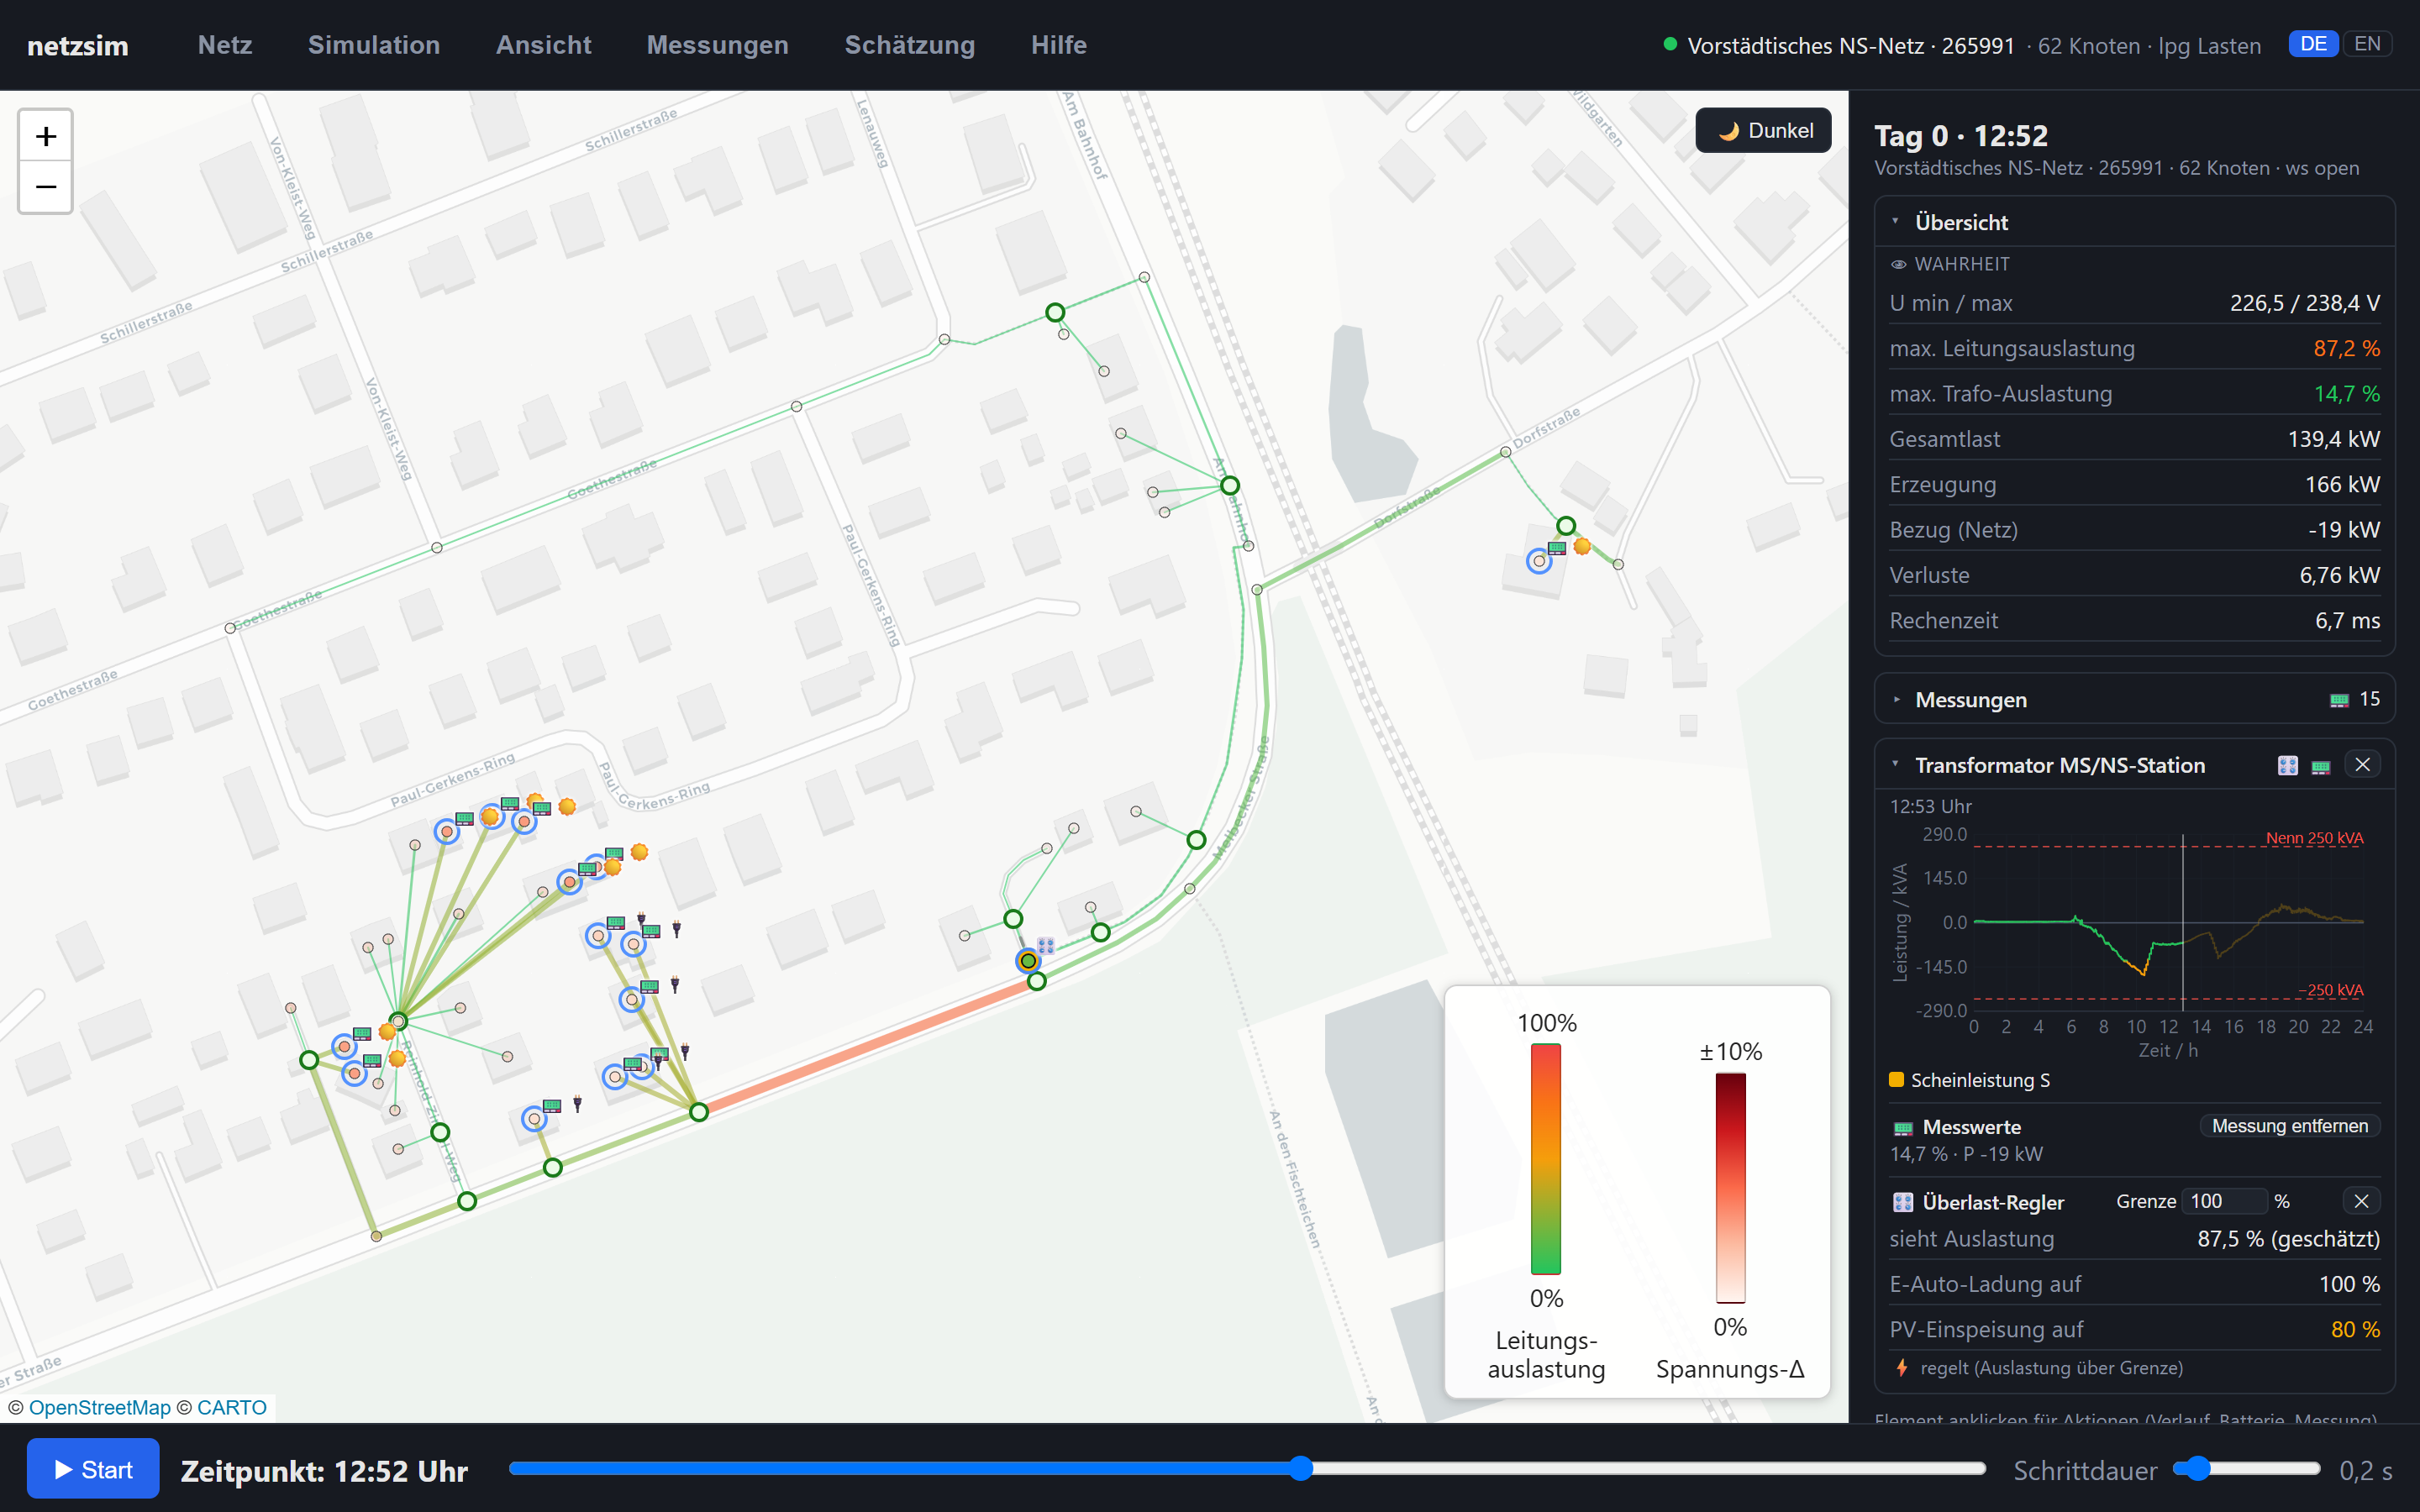
\includegraphics[width=\textwidth]{ui-regler}
  \caption{Netzregler an der Station im Referenzszenario~3 (12:50
    Uhr): Die Regler-Sektion zeigt \ui{sieht Auslastung}
    91{,}7\,\% (geschätzt) --- über der Grenze von 100\,\% hat er
    die \ui{PV-Einspeisung auf} 85\,\% gedrosselt, die E-Auto-Ladung
    blieb unangetastet. Die wahre maximale Leitungsauslastung ist
    dadurch von $\approx$110 auf 91\,\% gefallen; das mittlere
    Strangsegment auf der Karte ist noch orange gefärbt.}
  \label{fig:regler}
\end{figure}

\begin{beispiel}[Regelgüte = Beobachtbarkeit, an den Referenzszenarien]
Ein Netzregler an der Station (Grenze 100\,\%) verhält sich in den
drei Messkonzepten grundverschieden:
\begin{itemize}[nosep]
  \item \emph{Szenario 3 mit SMGW an PV und Wallboxen:} Die
    Schätzung sieht die Strangmitten-Überlast ($\approx$110\,\%),
    der Regler drosselt die PV auf 80\,\% --- die Wahrheit fällt
    auf $\approx$88\,\%, die E-Autos bleiben unangetastet.
  \item \emph{Szenario 3 nur mit Stationsmessung:} Der Regler sieht
    über die Schätzung nur $\approx$45\,\% und bleibt untätig ---
    die reale Überlast von $\approx$110\,\% besteht fort. Genau die
    Pointe des Szenarios: Was niemand misst, kann auch niemand
    regeln.
  \item \emph{Szenario 2 nur mit Stationsmessung:} Hier genügt die
    Stationsmessung --- die Schätzung rekonstruiert den überlasteten
    Strangkopf aus dem Summenfluss ($\approx$98\,\%), der Regler
    dimmt die E-Auto-Ladung auf 80\,\% und die Wahrheit sinkt von
    105 auf 95\,\%.
\end{itemize}
\end{beispiel}

\section{rONT: der regelbare Ortsnetztransformator}

Der zweite netzdienliche Aktor ist der \textbf{rONT} --- ein
Ortsnetztrafo mit Laststufensteller. Im Element-Menü eines
Transformators aktiviert ihn \ui{rONT aktivieren (Stufensteller)}:
Der Trafo erhält den typischen rONT-Stellbereich ($\pm 4$ Stufen à
1,5\,\%) und hält fortan die Spannung seiner NS-Sammelschiene in
einem Totband um den einstellbaren \ui{Sollwert} (Standard 230~V
$\pm$ 3,5~V). Auch der rONT sieht nur die Betreibersicht: die
Sammelschienen-Spannung aus dem dortigen Smart Meter, sonst aus der
Zustandsschätzung --- ohne Daten hält er seine Stufe. Pro
Regelhandlung schaltet er genau eine Stufe (ein mechanischer
Stufensteller springt nicht), schätzungsgespeist eine je neuem
Telegramm.

\begin{beispiel}[Spannung heben zur Abendspitze]
Vorstadtnetz zur Abendspitze: Die Sammelschiene liegt bei 225~V, das
tiefste Strangende bei 215~V. Sollwert auf 236~V stellen --- der rONT
schaltet in drei Schritten auf Stufe $-3$ ($+4{,}5\,\%$), die
Sammelschiene steht bei 235,6~V, und das Strangende gewinnt dieselben
$\approx$10~V (im Versuch: min.\ 225,6~V statt 215,4~V). Umgekehrt
schafft ein abgesenkter Sollwert mittags Platz für PV-Einspeisung ---
die Spannungsentkopplung der NS-Zelle von der MS-Ebene, ganz ohne
Netzausbau. Die Tagesgraphen zeigen wie bei den Überlast-Reglern den
\emph{ungeregelten} Tag; der rONT wirkt im Live-Lauf.
\end{beispiel}

Die Regler-Sektion zeigt laufend die aktuellen Stellgrößen
(\ui{E-Auto-Ladung auf} X\,\%, \ui{PV-Einspeisung auf} X\,\%, gelb
während der Drosselung) und den Status (\ui{regelt} /
\ui{bereit}); die \ui{Grenze} ist zwischen 20 und 150\,\%
einstellbar --- mit 80\,\% lässt sich präventives Engpassmanagement
zeigen, mit 120\,\% eine tolerante Betriebsführung. Szenarien
speichern platzierte Regler mit. \emph{Einschränkung:} Die
Tagesdiagramme zeigen stets den \emph{ungeregelten} Tag --- der
Regler wirkt in der laufenden Simulation, sein Effekt ist an den
Live-Werten und der Karte ablesbar.

\emph{Wichtig:} Laufzeit-Anlagen und -Regler gehören zum aktuell
geladenen Netz. Ein Netzwechsel setzt sie zurück --- wer ein Setup
behalten möchte, speichert es als Szenario
(Kapitel~\ref{ch:scenarios}).

% ===================================================================
\chapter{Reale Messdaten: PV-Tage und Strompreise}
\label{ch:realpv}

Liegt die Datei \texttt{data/real\_pv\_days.json} vor (erzeugt mit
\texttt{scripts/fetch\_real\_pv.py} aus den Minutenmesswerten einer
realen PV-Anlage), erscheint in der Live-Ansicht der
\ui{Tag}-Regler: Jeder Tag ist eine echte, gemessene Solarkurve,
normiert auf die Nennleistung und skaliert auf jede PV-Anlage im
Netz.

\begin{beispiel}
Der Datensatz der Beispielinstallation umfasst 37 Frühjahrstage.
Tag~3 ist wolkenlos --- eine glatte Glocke, die Rückspeisung baut
sich ruhig auf. Tag~11 ist Aprilwetter: Die PV-Leistung springt im
Minutentakt zwischen 20 und 100\,\%, auf der Karte flackern die
Leitungsfarben, und eine Batterie im \ui{Eigenverbrauch}-Modus
wechselt sichtbar hektisch zwischen Laden und Entladen. Der direkte
Tagesvergleich zeigt, warum Wolkendurchzug für Spannungsregelung
und Speichersteuerung das eigentlich harte Problem ist.
\end{beispiel}

Nur \emph{PV-Anlagen} folgen den Messtagen; Windkraft- und
Biogasanlagen (etwa in eigenen MS-Netzen, Kapitel~\ref{ch:gridedit})
behalten ihre eigenen Profile. Ein Netz ganz ohne PV bietet den
Tag-Regler nicht an.

Analog liefern gecachte aWATTar-Day-Ahead-Preise
(\texttt{data/awattar\_prices.json}, stündlich, dem jeweiligen
PV-Tag zugeordnet) die Preiskurven für die Batteriestrategie
\ui{Preis}: An sonnigen Tagen fallen die Mittagspreise --- die
Preis-Batterie kauft dann genau dann ein, wenn auch das Netz
entlastet werden müsste.

% ===================================================================
\chapter{Szenarien}
\label{ch:scenarios}

Ein Szenario sichert das komplette aktuelle Setup als
\emph{Rezept}, nicht als Momentaufnahme: gespeichert wird, \emph{wie}
der Zustand herzustellen ist (Netz, Lastkonfiguration, alle
nachträglichen Anlagen-Operationen, Batterien, Messungen,
Simulationszeitpunkt). Beim Laden wird diese Kette einfach neu
abgespielt. Der Vorteil: Die Dateien sind klein, lesbar und von Hand
anpassbar.

\begin{itemize}[nosep]
  \item \ui{Datei \(\to\) Szenario speichern\ldots} öffnet einen
    kleinen Dialog: Namen eintippen, \ui{Speichern} legt das
    aktuelle Setup ab.
  \item \ui{Datei \(\to\) Szenario laden} klappt die Liste der
    gespeicherten Szenarien als Untermenü aus; ein Klick spielt
    das Rezept vollständig ab und startet am gespeicherten Zeitpunkt,
    das $\times$ neben einem Eintrag löscht es.
\end{itemize}

Szenarien liegen als JSON-Dateien unter \texttt{data/scenarios/}.
Batterie-Ladezustände sind bewusst nicht Teil des Rezepts; nach dem
Laden starten Batterien bei 50\,\%.

\subsection*{Die drei Referenzszenarien}

Mitgeliefert werden drei aufeinander abgestimmte Referenzszenarien.
Gemeinsame Frage: Welche Fehlerfälle kann der Netzbetreiber per
Zustandsschätzung überhaupt sehen --- und wozu braucht er
SMGW-Messungen an Erzeugungsanlagen und Wallboxen
(Kapitel~\ref{ch:observability})? Alle drei starten kurz vor der
kritischen Zeit und bringen ihr Messkonzept (Stationsmessung + SMGW
an den Anlagen) mit.

\begin{enumerate}[nosep]
  \item \textbf{Bauernhof-PV 75 kW --- Spannungsüberhöhung:}
    ländliches Netz, 75-kWp-Anlage am 500-m-Strangende. Mittags
    steigt die Spannung dort auf $\approx$252~V --- direkt an der
    EN-50160-Grenze (253~V). Mit SMGW an der Anlage trifft die
    Schätzung die Überhöhung auf unter 1~V; entfernt man das SMGW,
    sieht der Netzbetreiber nur $\approx$245~V und ahnt nichts.
  \item \textbf{Feierabend-Laden --- NH-Sicherung löst aus:}
    Vorstadtnetz, 12 von 24 Haushalten am Hauptstrang laden
    17:00--18:30 gestaffelt (11~kW). Ab $\approx$18:45 trägt der
    Strangkopf $\approx$108\,\% / 243~A --- diesen Summenstrom sieht
    auch die NH-Strangsicherung, sie würde nach einiger Zeit
    auslösen. Schon die Stationsmessung findet die Überlast.
  \item \textbf{Mittags-Überlast --- unsichtbar für die
    NH-Sicherung:} gleicher Strang, hinten speisen acht PV-Anlagen
    (je 27~kWp) voll ein, vorn laden sechs E-Autos ihren
    PV-Überschuss (22~kW). Das mittlere Strangsegment trägt
    $\approx$110\,\% / 248~A, der Abgang an der Station aber nur
    $\approx$100~A (45\,\%): Die Sicherung sieht diesen Strom nie.
    Ohne SMGW schätzt der Netzbetreiber das Segment auf
    $\approx$4\,\% --- mit SMGW an PV und Wallboxen exakt. Das
    Kernargument für die Messung dezentraler Anlagen.
  \item \textbf{Feierabend im Bezirk --- Engpass unsichtbar für jede
    Zelle:} das vertikale Szenario auf dem ganzen MS-Bezirk ---
    ausführlich in Kapitel~\ref{ch:vertikal}.
\end{enumerate}

\begin{beispiel}[Ein Rezept von innen]
Das Rezept von Szenario 1 zeigt das Format (gekürzt):

\begin{lstlisting}
{
  "version": 1,
  "name": "1 Bauernhof-PV 75 kW - Spannungsüberhöhung",
  "grid_id": "lv_rural_3150_300266",
  "loadgen": {
    "archetypes": ["CHR01", "CHR03", "CHR05", "CHR07",
                    "CHR16", "CHR30", "CHR22", "CHR52"],
    "mode": "round_robin", "seed": 0, "scale": 1.0,
    "power_factor": 0.95
  },
  "der_ops": [ { "op": "add_pv", "bus": 24, "kwp": 75.0 } ],
  "batteries": [],
  "measurements": { "node_buses": [24], "trafo_idxs": [0],
                    "mode": "full" },
  "engine": { "day": 0, "step": 660, "interval_seconds": 0.2 }
}
\end{lstlisting}

Zum Anpassen genügt ein Texteditor: \texttt{"kwp": 100.0}
verschärft die Überhöhung, ein Eintrag in \texttt{"batteries"}
(z.\,B. \texttt{\{"bus": 24, "capacity\_kwh": 20, "power\_kw": 10,
"mode": "self"\}}) stellt die Gegenmaßnahme gleich mit ins Rezept.
\end{beispiel}

% ===================================================================
\chapter{Vertikale Integration: vom Ortsnetz zum Bezirk}
\label{ch:vertikal}

Bisher spielte alles in \emph{einem} Ortsnetz. Reale Smart Grids sind
aber vertikal geschichtet: Unter einem Mittelspannungsring hängen
Dutzende \textbf{Ortsnetz-Zellen} --- jede mit eigener Station, eigener
Messung, eigenen flexiblen Anlagen. netzsim bildet diese Schichtung
vollständig ab: Der Picker bietet dafür den \emph{ländlichen MS-Bezirk
3150} an --- 475 Knoten, ein 10-kV-Ring, 157 Ortsnetz-Zellen, davon
drei als voll ausgebaute Straßennetze (die übrigen als Summenlast an
ihrer Station, wie es auch ein Netzberechnungsprogramm täte).

\section{Drei vertikale Bausteine}

\begin{description}
  \item[Digitale Ortsnetzstationen.] Das Messungen-Preset
    \ui{Digitale Ortsnetzstationen} setzt genau \emph{eine}
    Stationsmessung je Zelle --- den Trafo-Zähler, wo die Station
    ausgebaut ist, sonst die Messung am speisenden MS-Bus. Mehr
    Messtechnik hat ein Verteilnetzbetreiber flächig selten.
  \item[Hierarchische Schätzung.] Auf Bezirken schätzt die WLS
    \emph{zweistufig}, wie ein VNB es schichtet: Jede ausgebaute
    Zelle schätzt lokal; ihr \emph{Randfluss} --- gemessen, sonst
    zellgeschätzt, sonst Profilannahme --- speist die Schätzung auf
    dem MS-Ring. Einstellbar in der \ui{Schätz-Richtlinie}
    (\ui{Vertikale Schätzung}: automatisch/hierarchisch/monolithisch).
  \item[Netzampel-Kaskade.] An jeder Zellstation lässt sich per
    Element-Menü eine \textbf{Steuerbox} (Zellenregler) platzieren;
    am UW-Bus der \textbf{MS-Koordinator}. Der Koordinator sieht nur
    die MS-Ebene (Messung und Schätzung, nie die Wahrheit), drosselt
    aber nichts selbst: Er sendet sein Ampel-Signal an alle
    Steuerboxen, die es lokal als Obergrenze übernehmen --- der
    Befehlsweg braucht eine Steuerbox, kein Messgerät. Die
    Seitenpanel-Sektion \ui{Netzampel} zeigt Koordinator-Status,
    Signale und wie viele Zellen gerade dimmen; dimmende Stationen
    tragen auf der Karte einen roten Ring.
\end{description}

\section{Referenzszenario 4: Feierabend im Bezirk}

Das Szenario \ui{4 Feierabend im Bezirk} lädt den Bezirk mit
LPG-Haushalten und legt ab 17~Uhr an die 42 Stationen eines
Ringstrangs gestaffelte Wallbox-Blöcke von je 200~kW --- zusammen
eine 8,4-MW-Feierabendwelle, wie sie ein E-Mobilitäts-Hochlauf
erzeugt. Steuerboxen an diesen 42 Stationen und digitale
Ortsnetzstationen überall sind im Rezept enthalten; die Uhr startet
17:40.

\begin{enumerate}[nosep]
  \item \textbf{Jede Zelle für sich: unauffällig.} Die höchste
    Stationsmessung im ganzen Bezirk zeigt \textbf{60,8\,\%}, die
    drei ausgebauten Zellen liegen bei 10--65\,\% --- kein einziges
    Messgerät meldet ein Problem.
  \item \textbf{Die MS-Sicht sieht ihn doch.} In der Sicht
    \ui{Schätzung} rekonstruiert die hierarchische WLS aus den 157
    Randflüssen den Ring --- und färbt ein Segment rot:
    \textbf{108,3\,\%} (die Wahrheit: 108,3\,\% --- die Schätzung
    trifft exakt, denn durch die Stationsmessungen ist jeder
    Randfluss bekannt). Der Engpass liegt \emph{zwischen} den
    Stationen: Genau wie die NH-Sicherung in Szenario~3 kann keine
    einzelne Zellmessung ihn sehen (Abbildung~\ref{fig:vertsch}).
  \item \textbf{Die Netzampel regelt ihn ab.} Klick auf den UW-Bus
    $\to$ \ui{Netzampel-Koordinator (MS) platzieren} (Grenze
    100\,\%). Der Koordinator sieht die Überlast über die Schätzung,
    setzt das EV-Signal auf \textbf{75\,\%}, alle 42 Steuerboxen
    führen es aus --- das Segment fällt auf \textbf{87\,\%} und
    bleibt stabil im Hystereseband; auf der Karte markieren rote
    Ringe die dimmenden Stationen (Abbildung~\ref{fig:vertampel}).
    Jede Zelle hat nur ein Viertel ihrer Wallbox-Leistung verloren
    --- \emph{gemeinsam} reicht das.
\end{enumerate}

\begin{figure}[htbp]
  \centering
  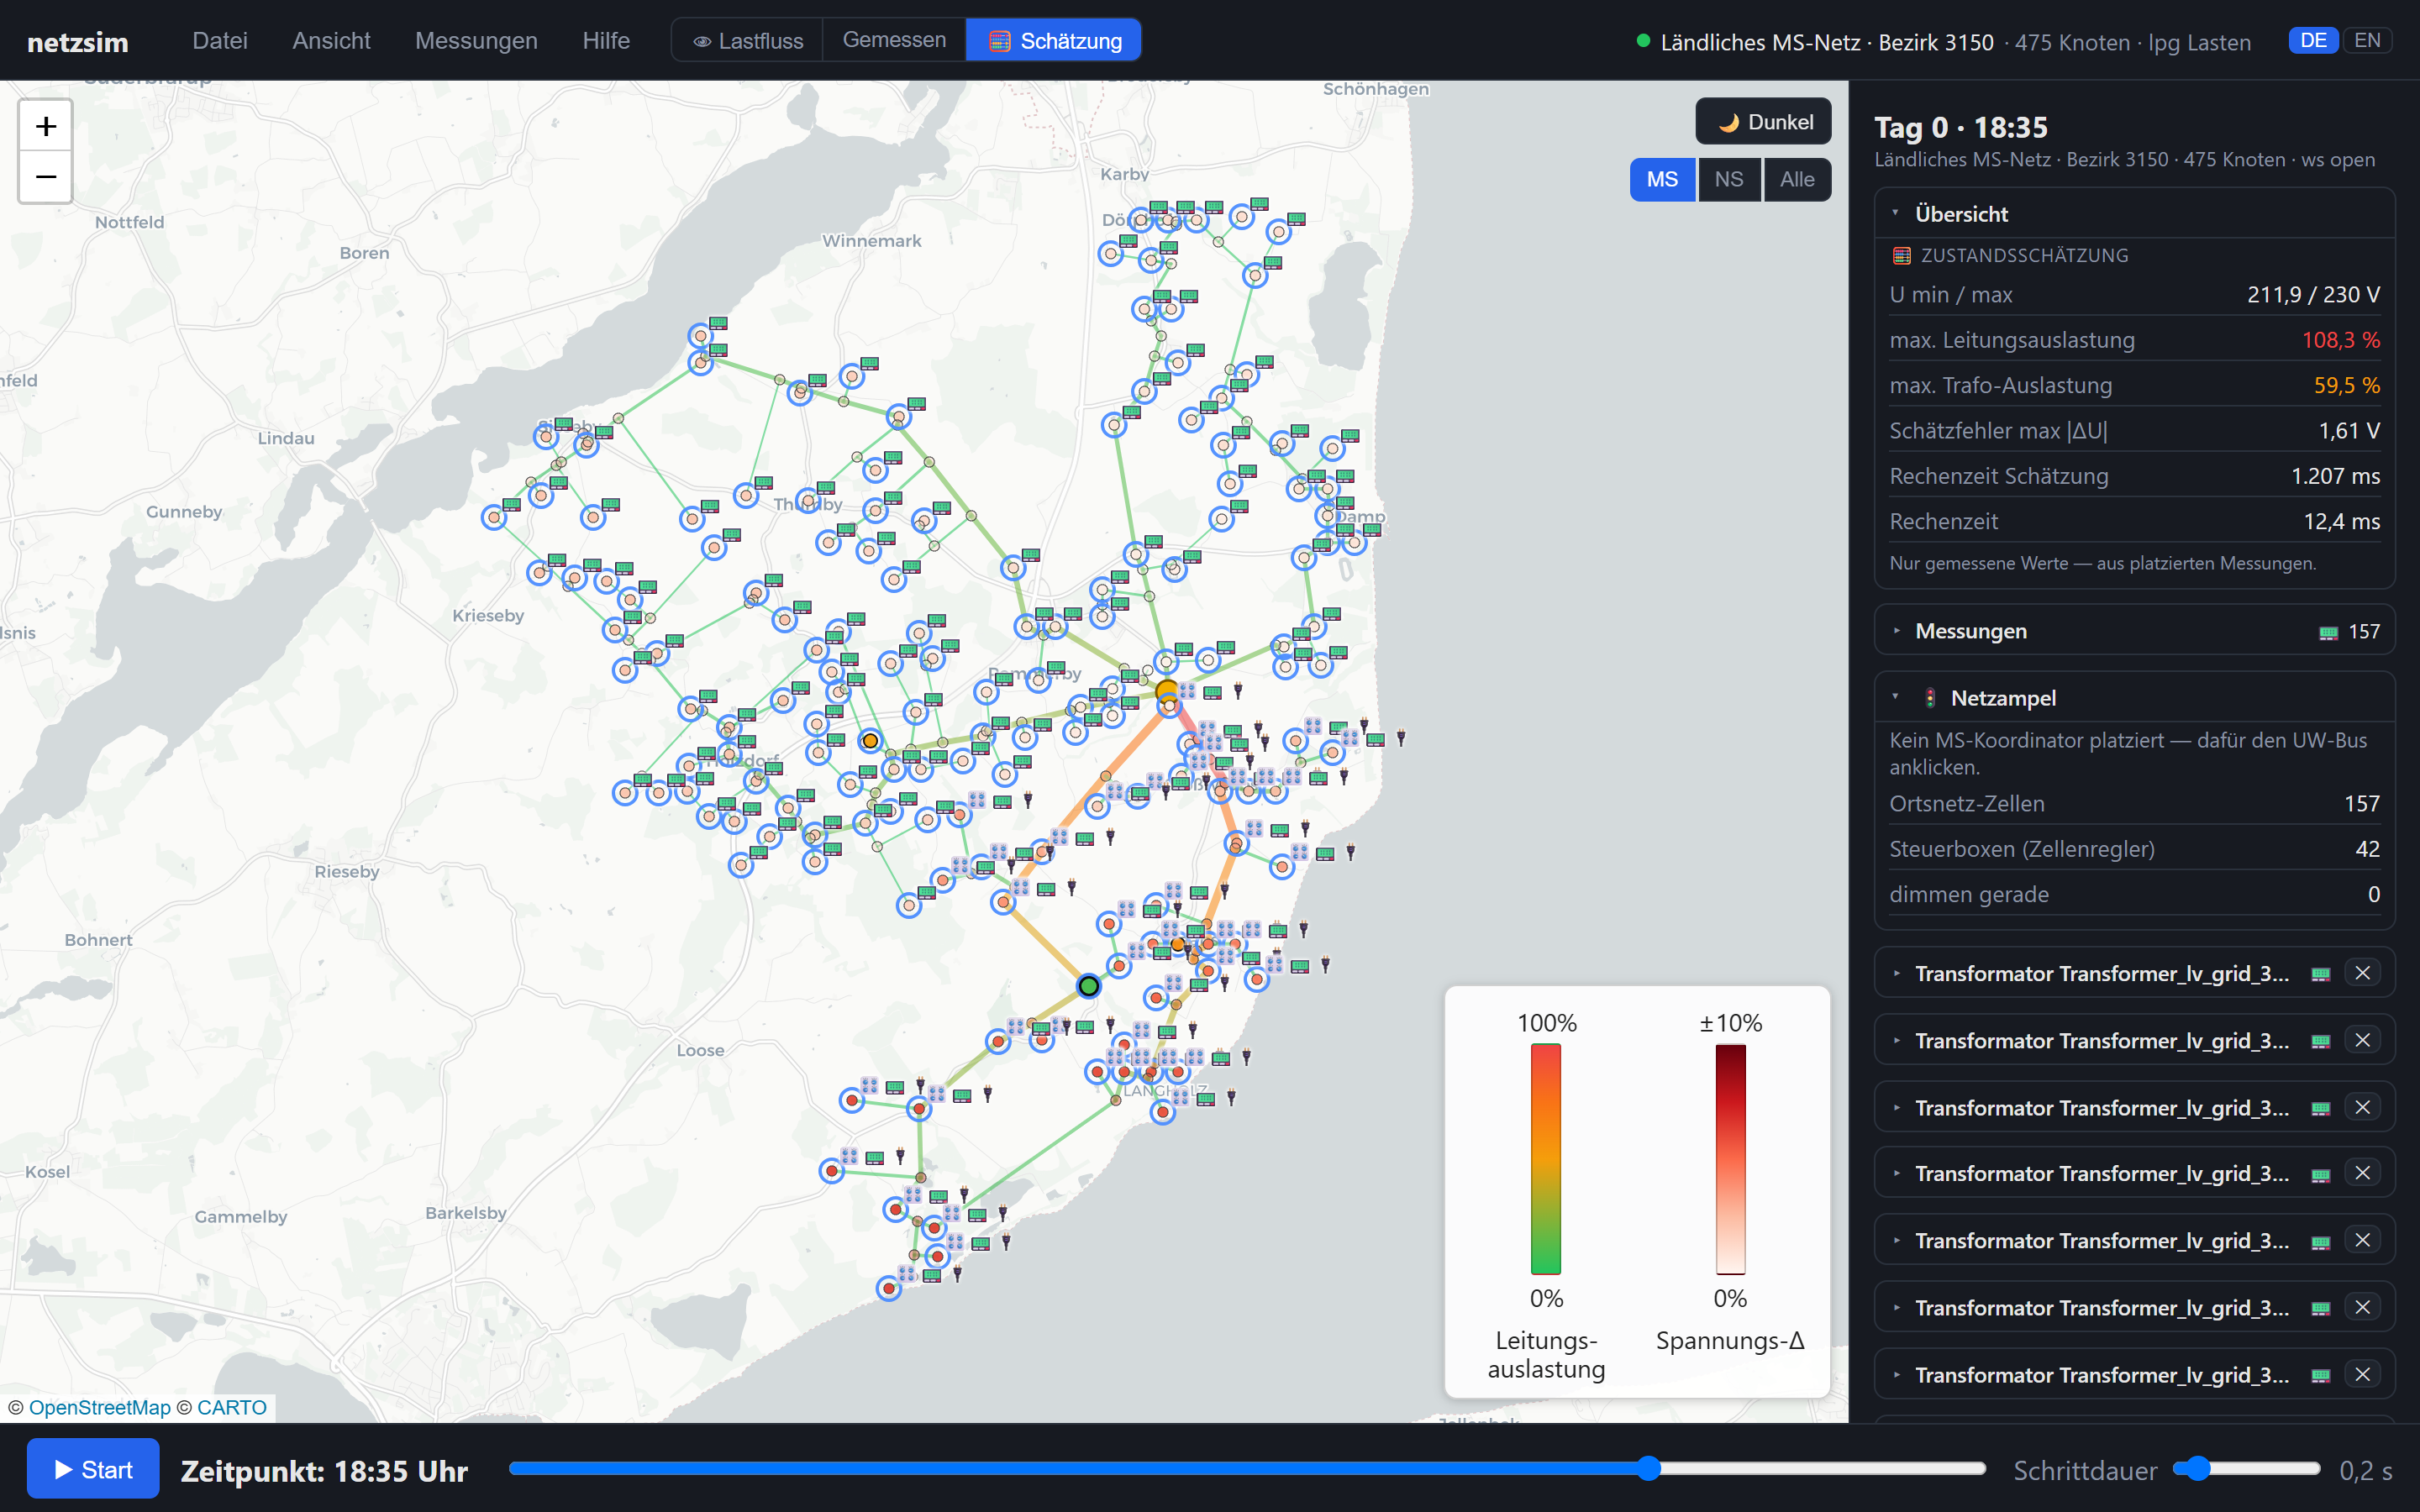
\includegraphics[width=\textwidth]{ui-vertikal-schaetzung}
  \caption{Sicht \ui{Schätzung} auf dem Bezirk um 18:34: Die
    hierarchische Schätzung rekonstruiert aus den Randflüssen der
    digitalen Ortsnetzstationen das überlastete Ringsegment
    (108\,\%, rot) --- das keine einzelne Stationsmessung sieht
    (Maximum: 60,8\,\%). Die \ui{Netzampel}-Sektion rechts zählt
    157 Zellen und 42 Steuerboxen, noch dimmt keine.}
  \label{fig:vertsch}
\end{figure}

\begin{figure}[htbp]
  \centering
  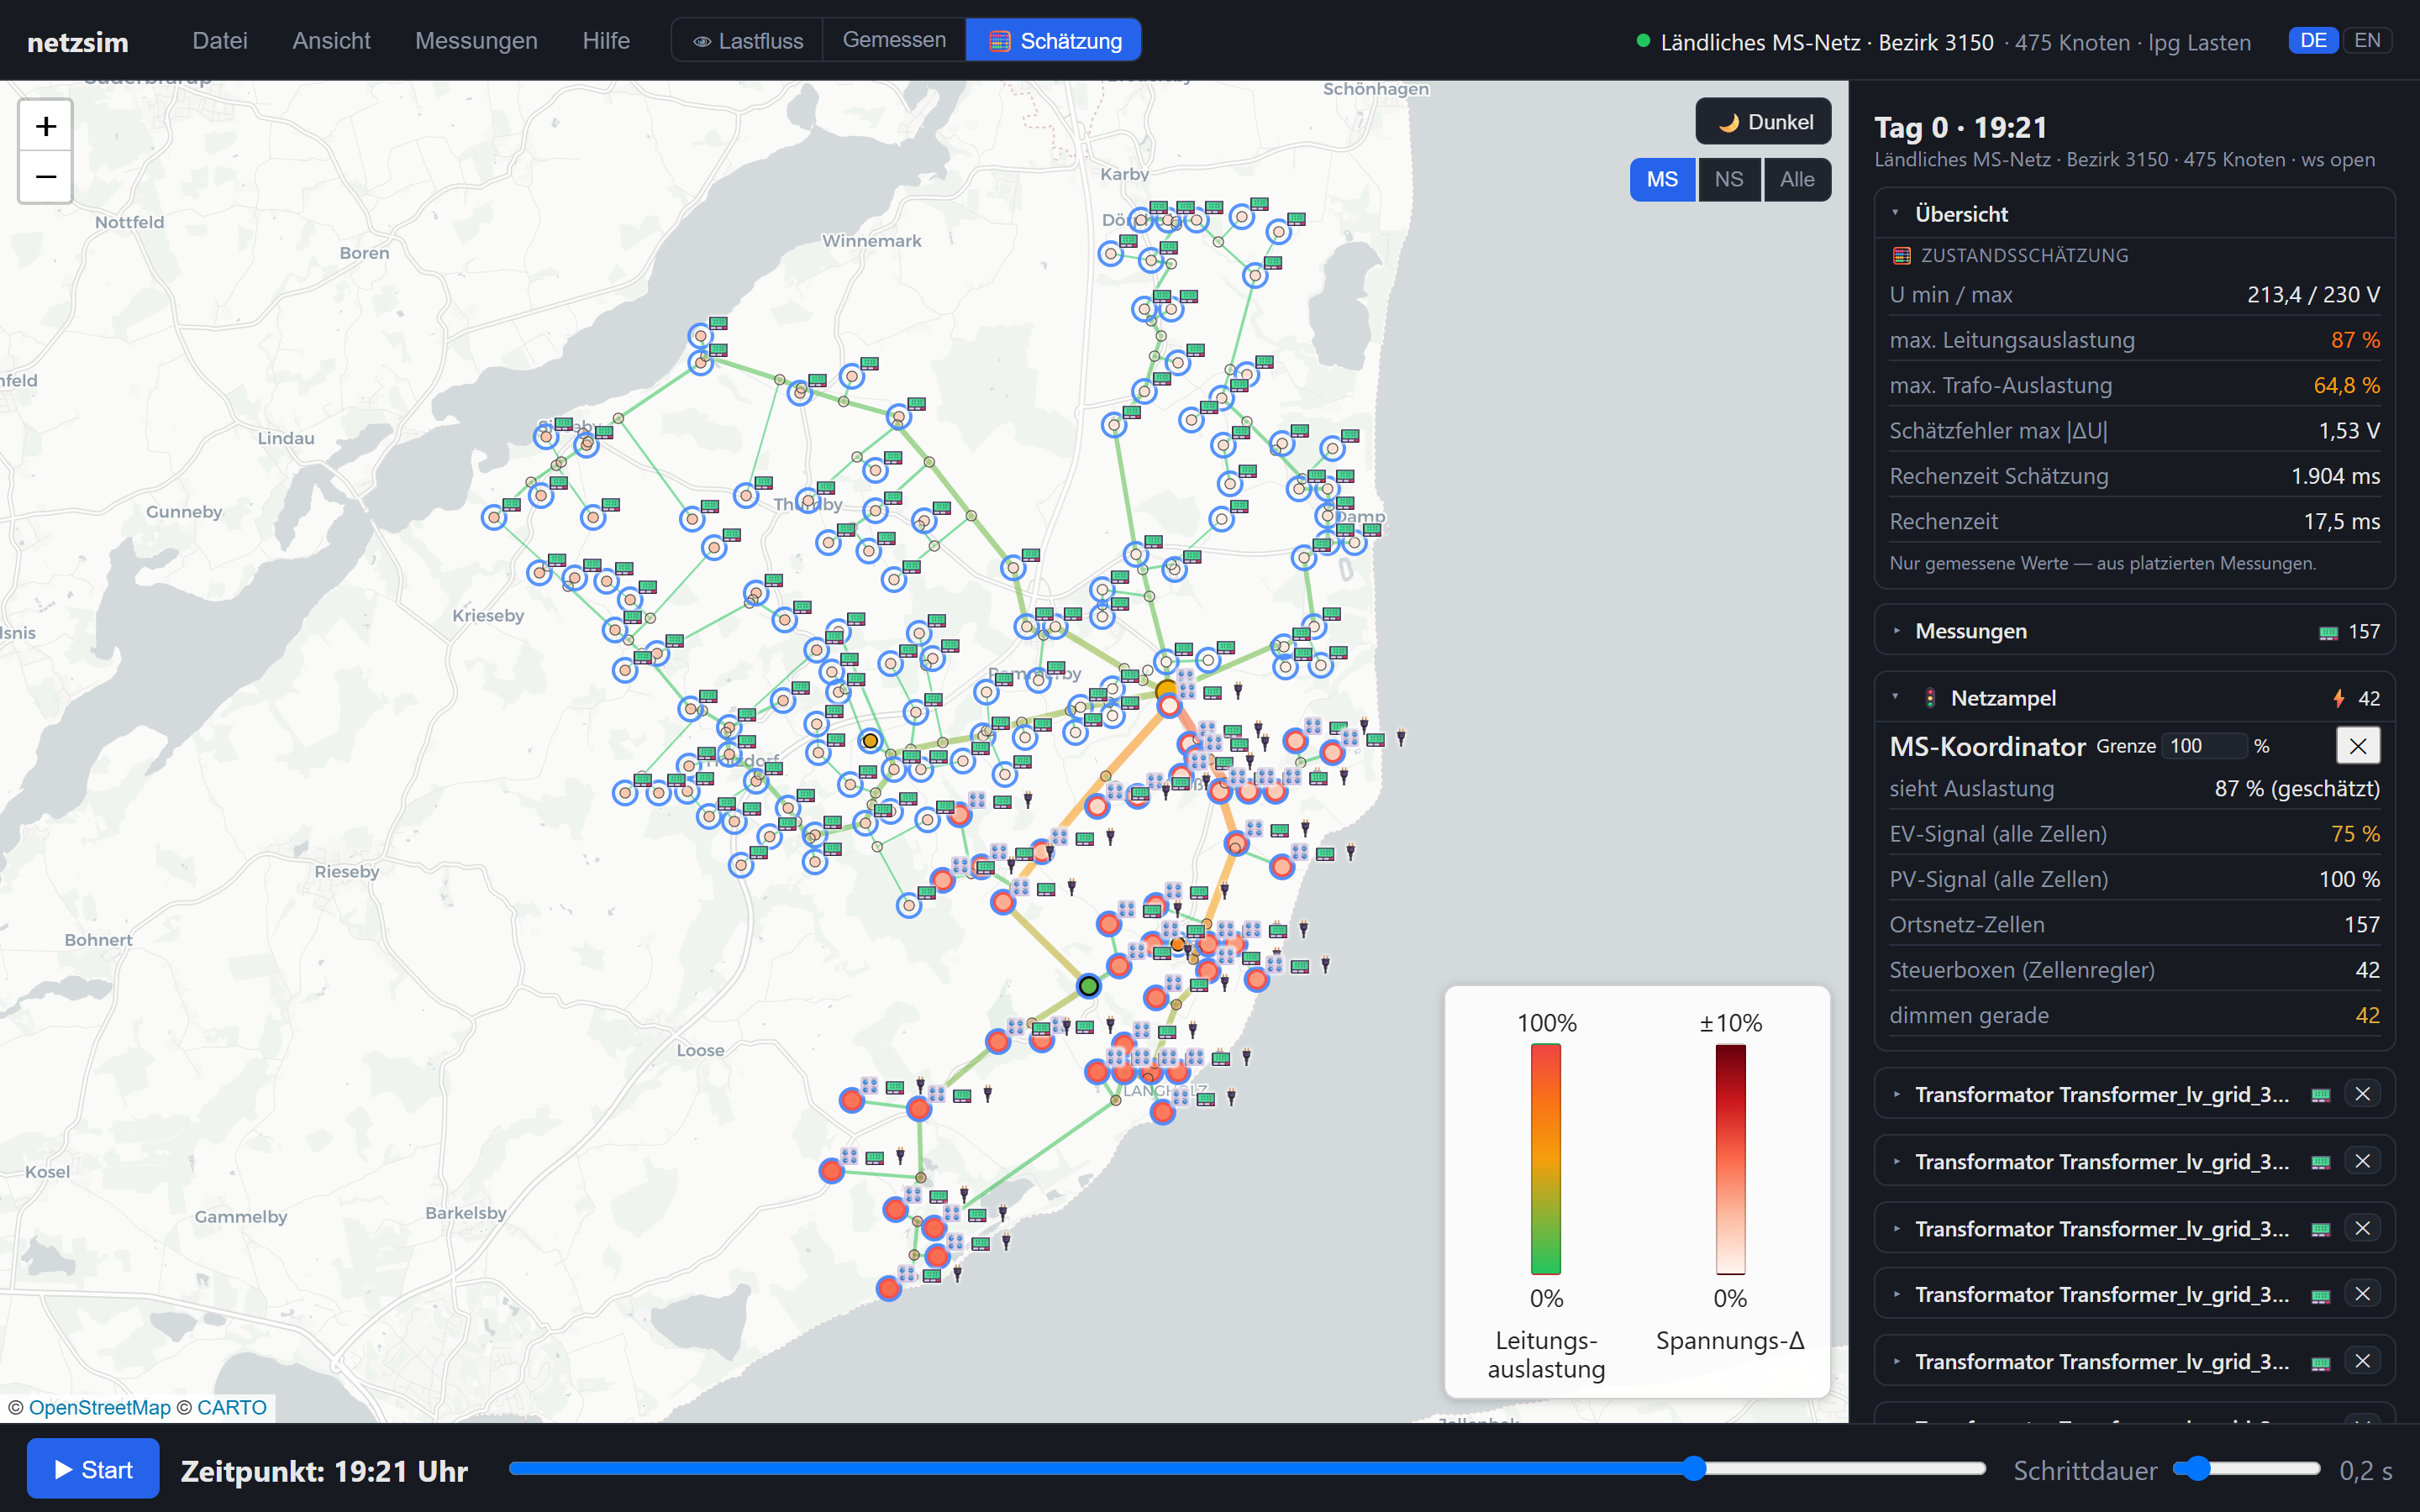
\includegraphics[width=\textwidth]{ui-vertikal-ampel}
  \caption{Nach dem Platzieren des MS-Koordinators (19:21): Er sieht
    87\,\% (geschätzt), sein EV-Signal steht auf 75\,\%, alle 42
    Steuerboxen dimmen (rote Ringe an den Stationen des Strangs) ---
    das Segment ist zurück unter der Grenze und pendelt sich im
    Hystereseband ein.}
  \label{fig:vertampel}
\end{figure}

Merksatz des Kapitels: \emph{Beobachtbarkeit und Steuerbarkeit müssen
dieselbe Ebene erreichen.} Die Zellenmessungen allein sehen den
MS-Engpass nicht; erst ihre Randflüsse machen ihn auf der Ebene
darüber sichtbar --- und erst die Kaskade zurück in die Zellen kann
ihn beheben.

% ===================================================================
\chapter{Daten exportieren}
\label{ch:export}

Alles, was die Simulation rechnet, lässt sich als \textbf{CSV-Paket}
herunterladen --- für die Auswertung in Python, MATLAB oder Excel und
als Datengrundlage für Übungsblätter. Beide Wege leben im Menü
\ui{Datei} (Abbildung~\ref{fig:export}) und erzeugen identisch
aufgebaute Pakete:

\begin{description}
  \item[\ui{Tage exportieren\ldots}] --- der Standardweg. Der
    Dialog fragt die gewünschte Anzahl Tage ab; sie wird
    \emph{offline} so schnell wie möglich durchsimuliert, ohne auf
    die beschleunigte Uhr zu warten: zwei volle Tage des
    Vorstadtnetzes rechnen in etwa einer Minute, live wären es 48
    Minuten. Gerechnet wird die \emph{echte} Live-Physik der
    aktuellen Konfiguration: Batterien starten bei 50\,\% und
    integrieren über Mitternacht hinweg, Überlast-Regler regeln im
    geschlossenen Kreis, bei geladenen PV-Messtagen ist jeder
    exportierte Tag ein anderer realer Solartag. Das Häkchen
    \ui{mit Zustandsschätzung} im selben Dialog entscheidet, ob die
    Schätzung mitläuft --- im Modus TAF~9/10/14 rechnet sie
    minütlich und dominiert dann die Exportdauer deutlich. Während
    des Exports zeigt eine Zeile im \ui{Datei}-Menü Fortschritt und
    Restzeit (\ui{Abbrechen} behält das bereits Gerechnete); die
    Simulation läuft währenddessen normal weiter, rechts in der
    Menüleiste erscheint ein Fortschritts-Chip, der auch bei
    geschlossenem Menü sichtbar bleibt.
  \item[\ui{Live-Sitzung aufzeichnen}] --- für interaktive
    Vorführungen: Ab dem Klick wird jeder Simulationsschritt
    mitgeschrieben, \emph{inklusive aller Eingriffe} (Anlagen
    dazuklicken, Regler platzieren, Messmodus wechseln). Ein rotes
    \ui{REC}-Zeichen in der Menüleiste zählt die Schritte mit; ein
    Netzwechsel beendet die Aufzeichnung automatisch sauber ---
    eine Aufzeichnung gehört immer zu genau einer Konfiguration.
\end{description}

Fertige Pakete listet das Untermenü \ui{Datei \(\to\)
Aufzeichnungen}: Ein Klick lädt das ZIP, das $\times$ daneben
löscht. Auf dem Server liegen die Pakete unter
\texttt{data/recordings/}. Die beiden Status-Chips (rotes \ui{REC},
Export-Fortschritt) sind klickbar und öffnen direkt das
\ui{Datei}-Menü.

\begin{figure}[htbp]
  \centering
  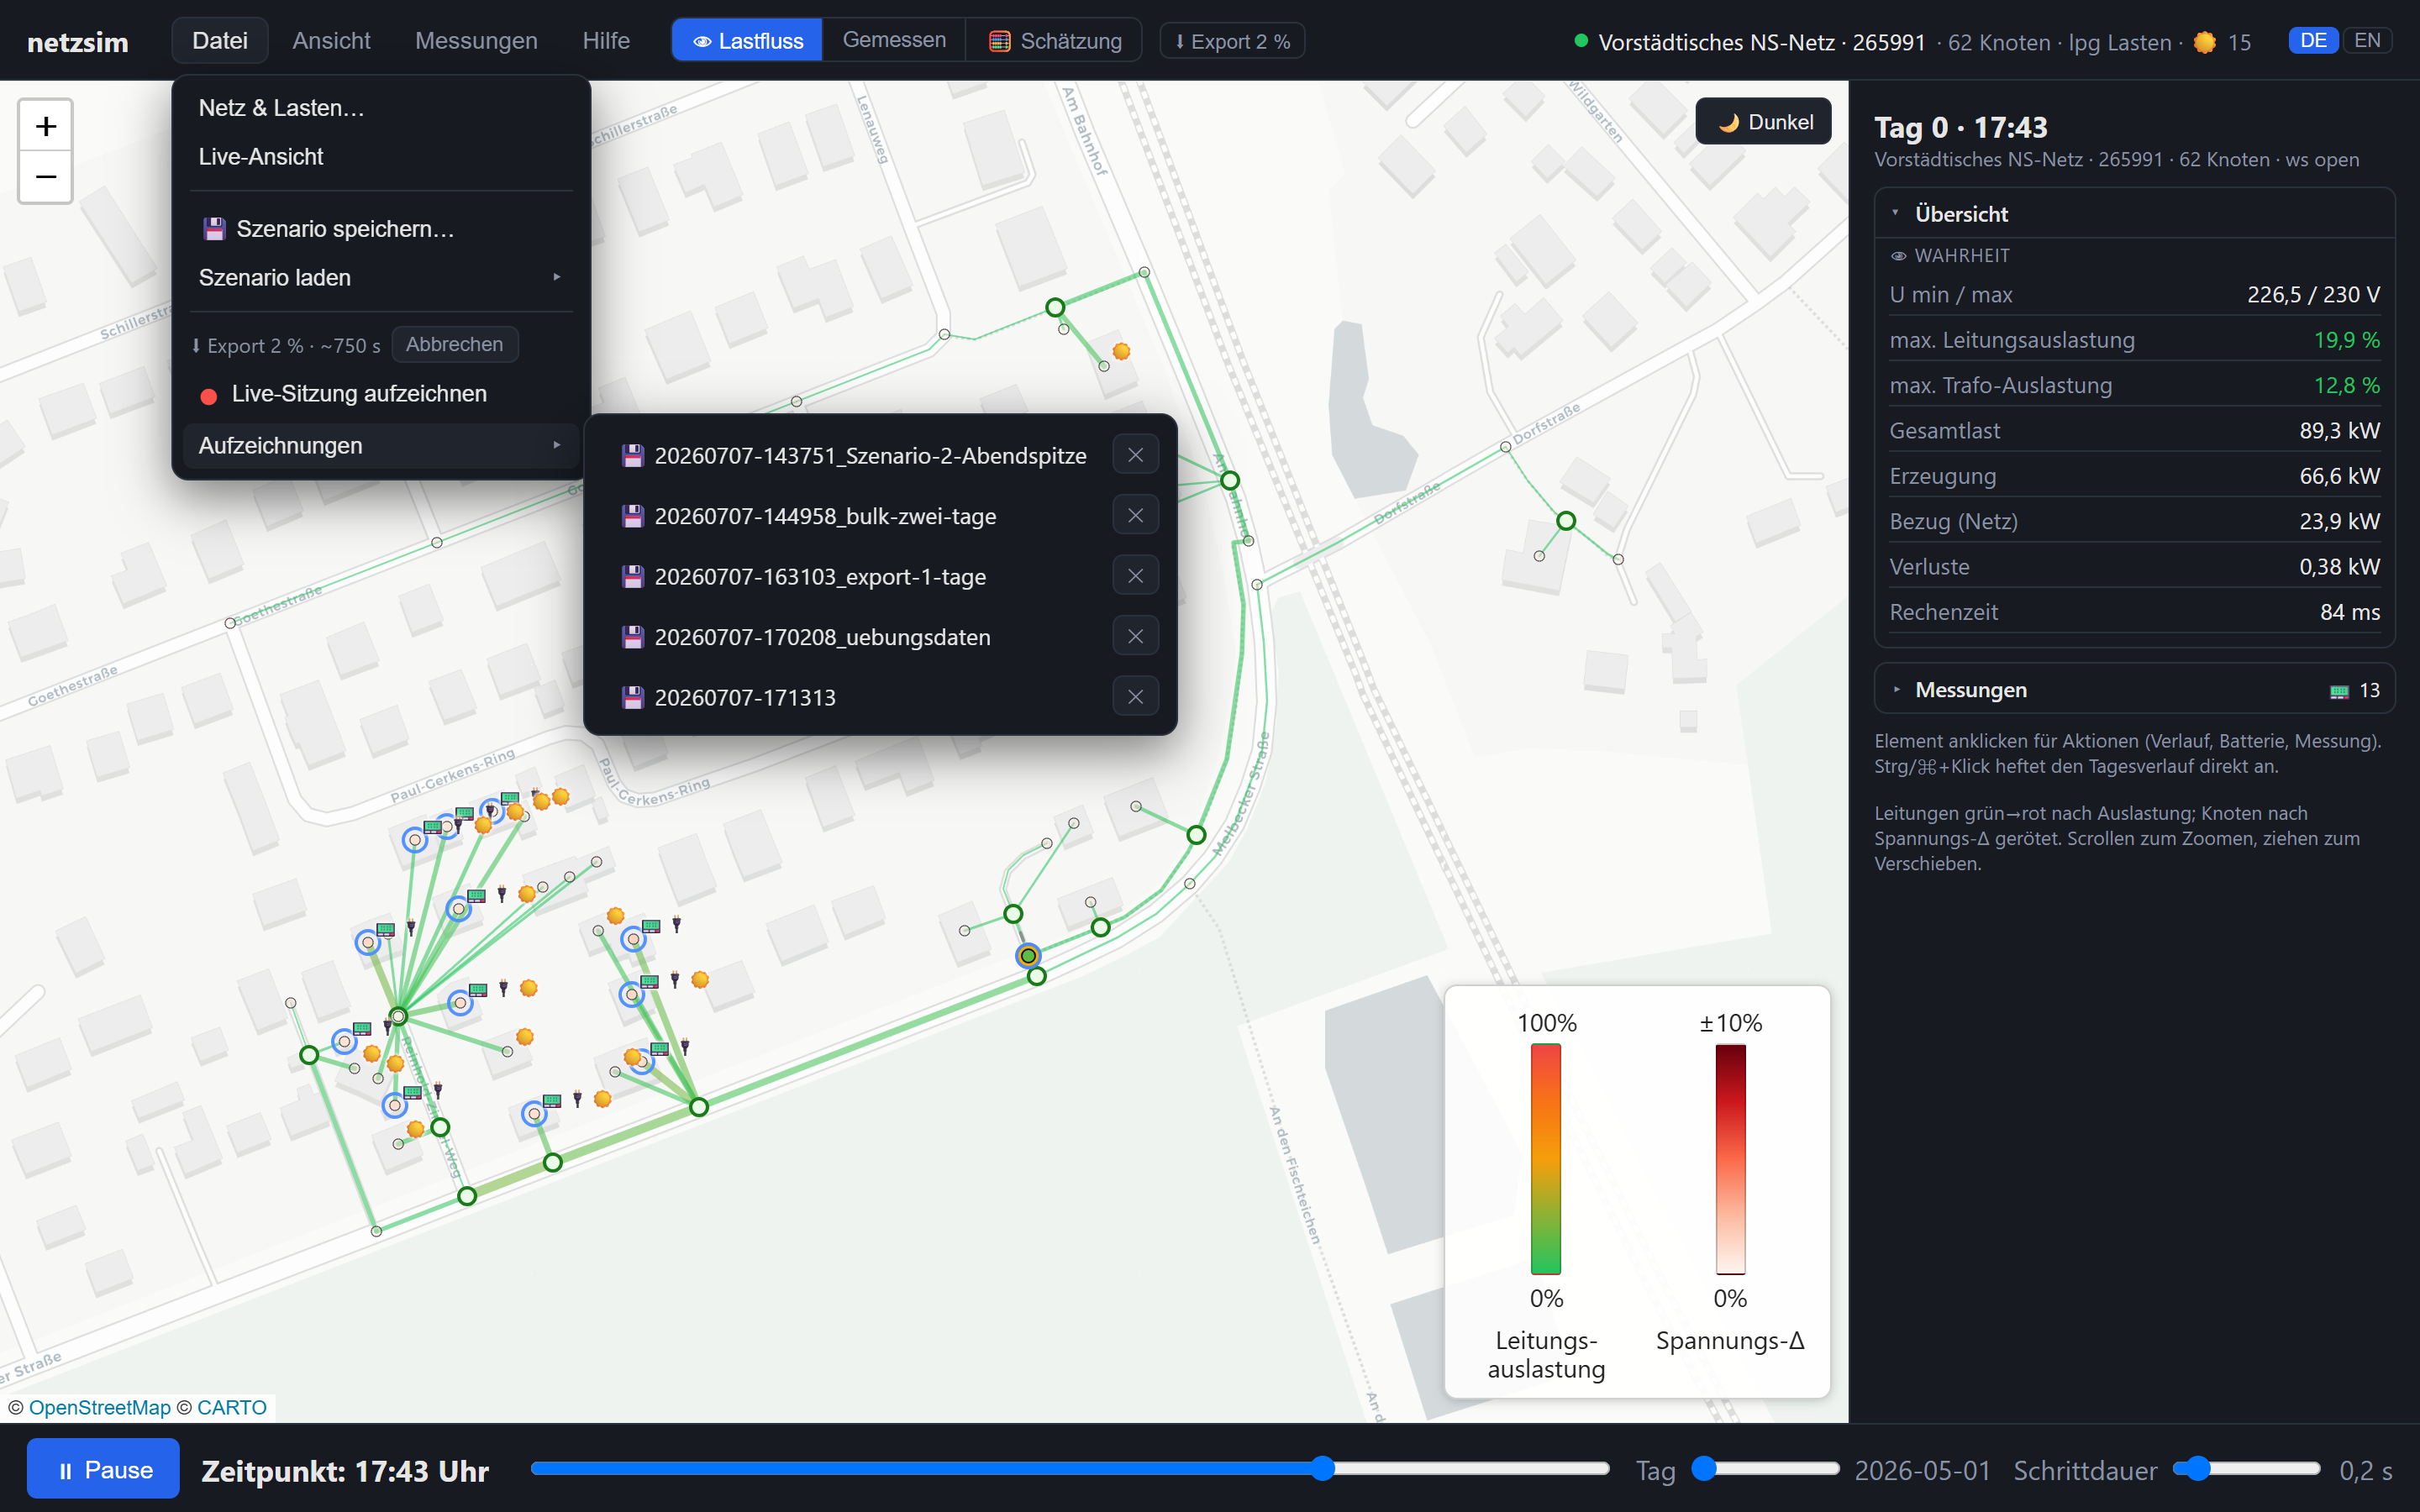
\includegraphics[width=\textwidth]{ui-export}
  \caption{Daten-Export im Menü \ui{Datei}: oben der laufende
    Tages-Export mit Fortschritt und \ui{Abbrechen}, darunter der
    Aufzeichnungs-Umschalter und das Untermenü \ui{Aufzeichnungen}
    mit den fertigen Paketen zum Download; rechts in der Menüleiste
    der Fortschritts-Chip, der auch bei geschlossenem Menü sichtbar
    bleibt.}
  \label{fig:export}
\end{figure}

\section{Der Inhalt eines Pakets}

Ein Paket ist ein ZIP mit \emph{tidy} CSV-Dateien (Komma-getrennt,
Punkt als Dezimalzeichen, UTF-8 --- direkt lesbar für pandas \&
Co.; leere Felder bedeuten \glqq nicht verfügbar\grqq):

\begin{center}
\small
\begin{tabularx}{\textwidth}{@{}lX@{}}
\toprule
Datei & Inhalt (je Zeile: Tag, Schritt, Uhrzeit, \ldots) \\
\midrule
\texttt{metadata.json} & das Rezept: Netz, Lastkonfiguration, Messkonzept, Schätz-Richtlinie, Schrittdauer, Version \\
\texttt{summary.csv} & Systemkennzahlen je Schritt (U min/max, Auslastungen, Bilanz) \\
\texttt{buses.csv} & Spannung und Einspeisung je Knoten und Schritt \\
\texttt{lines.csv} & Strom, Auslastung, Wirkfluss je Leitung und Schritt \\
\texttt{trafos.csv} & Auslastung und OS-Leistung je Transformator und Schritt \\
\texttt{batteries.csv}, \texttt{controllers.csv} & SOC/Leistung bzw.\ Live-Stellgrößen \\
\texttt{measurements\_*.csv} & \emph{nur} Messwerte platzierter Geräte, im TAF-Raster \\
\texttt{estimated\_*.csv} & die Zustandsschätzung, ein Block je Schätz-Zeitpunkt \\
\texttt{observed\_summary.csv} & Kennzahlen aus Sicht der Messungen \\
\bottomrule
\end{tabularx}
\end{center}

Dateien entstehen nur, wenn es etwas zu schreiben gibt --- ein Netz
ohne Batterien enthält keine \texttt{batteries.csv}. Und die
Ebenen-Treue aus Kapitel~\ref{ch:observability} gilt auch hier: Im
strikten Modus (\texttt{NETZSIM\_EXPOSE\_GROUND\_TRUTH=false})
enthält das Paket \emph{keine} Wahrheitsdateien, sondern nur
Messwerte und Schätzung.

\begin{beispiel}[Übungsdaten in drei Zeilen auswerten]
Drei exportierte Tage, geöffnet in Python:
\begin{lstlisting}
import pandas as pd
b = pd.read_csv("buses.csv")
b[b["index"] == 24].plot(x="step", y="vm_pu")  # Spannung am Strangende
\end{lstlisting}
Für Übungsblätter besonders nützlich: Den Studierenden nur
\texttt{measurements\_nodes.csv} und \texttt{metadata.json}
aushändigen --- also exakt das, was ein Netzbetreiber hätte --- und
die Aufgabe stellen, daraus den Netzzustand zu rekonstruieren. Die
zurückgehaltene \texttt{buses.csv} ist die Musterlösung.
\end{beispiel}

\emph{Dauerbetrieb:} Mit \texttt{NETZSIM\_RECORD=true} zeichnet der
Server von sich aus alles auf und beginnt bei jedem Netzwechsel ein
neues Paket --- praktisch für Laborrechner, auf denen nachträglich
nachvollziehbar sein soll, was simuliert wurde.

% ===================================================================
\chapter{Eigene Netze zeichnen (gridedit)}
\label{ch:gridedit}

Mit dem Schwesterwerkzeug \emph{gridedit} lassen sich eigene Netze
von Hand auf einer OpenStreetMap-Karte zeichnen und direkt in den
Netzkatalog exportieren (Abbildung~\ref{fig:gridedit}).

\begin{figure}[htbp]
  \centering
  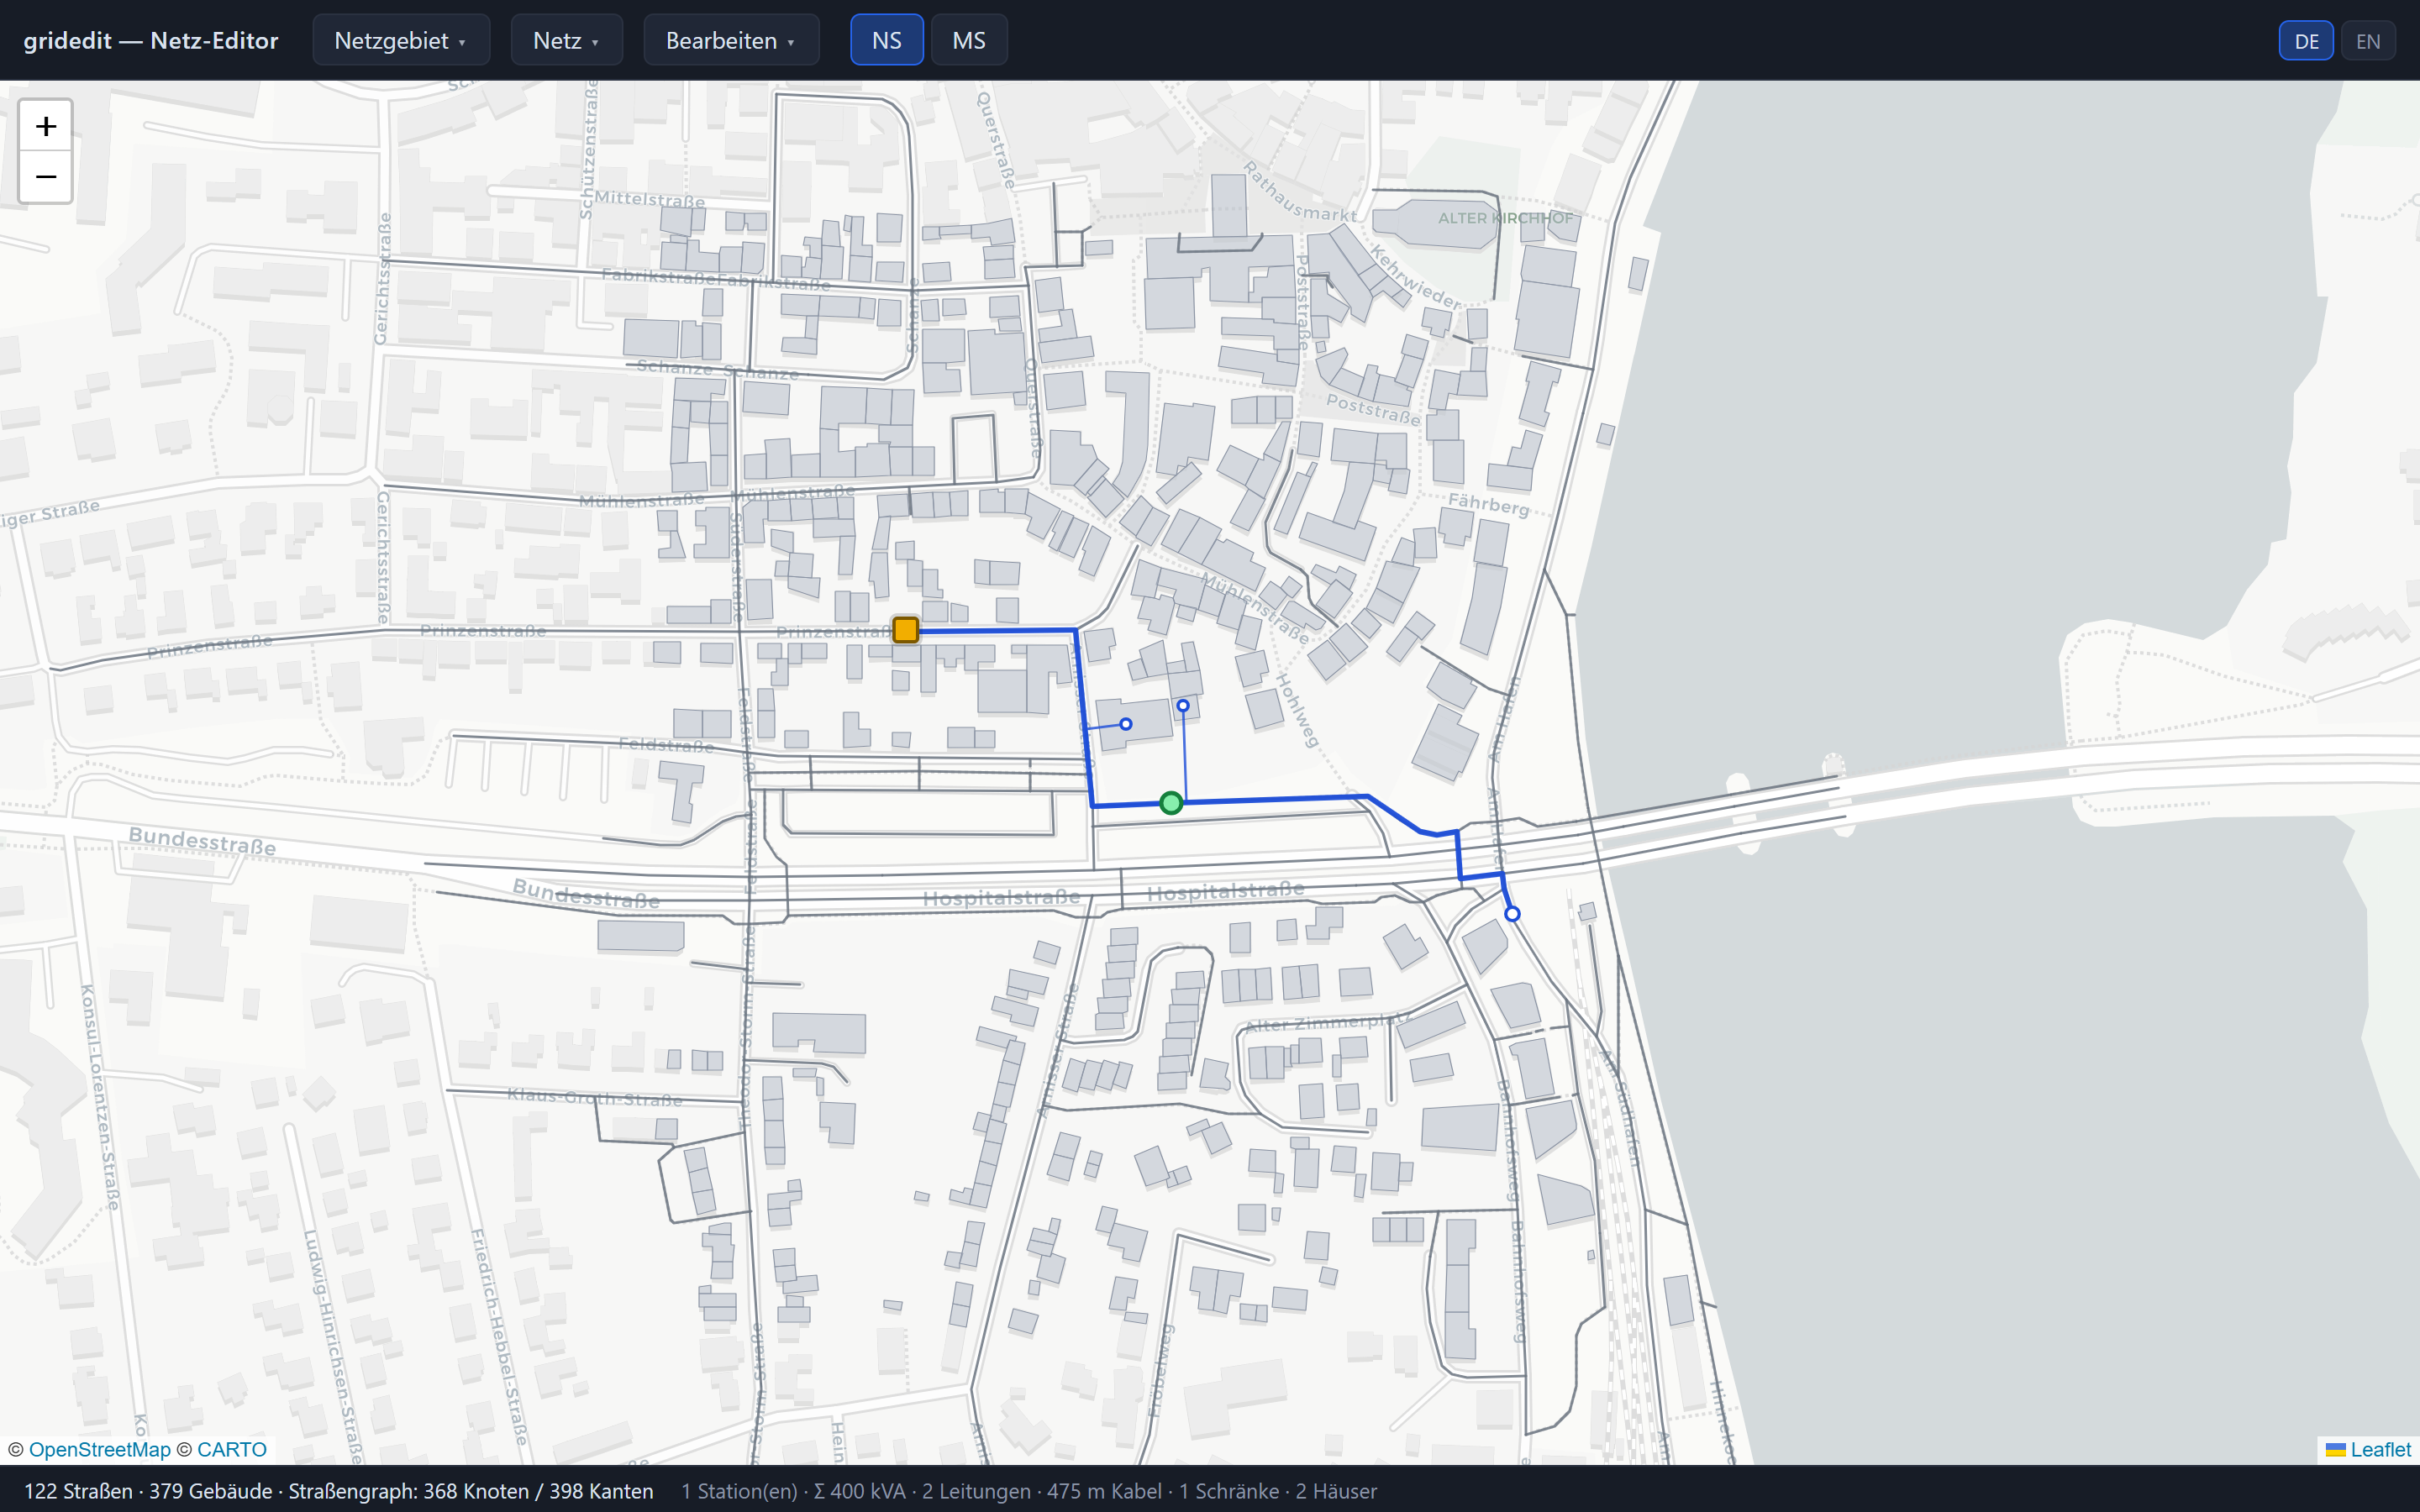
\includegraphics[width=\textwidth]{gridedit}
  \caption{Der Netz-Editor \emph{gridedit}: Ortsnetztransformator
    (orange), straßengeführtes NS-Hauptkabel (blau), Kabelverteiler
    (grün) und Hausanschlüsse; oben die Menüs \ui{Netzgebiet},
    \ui{Netz}, \ui{Bearbeiten} sowie der Ebenenumschalter NS/MS.}
  \label{fig:gridedit}
\end{figure}

\section{Ein Niederspannungs-Ortsnetz zeichnen}

Der typische Ablauf, hier für ein kleines Dorf:

\begin{enumerate}[nosep]
  \item \ui{Netzgebiet}: Kartenausschnitt aufziehen --- gridedit lädt
    Straßen und Gebäude aus OpenStreetMap (im Beispielausschnitt
    122 Straßen, 379 Gebäude).
  \item \ui{Transformator platzieren}: Klick auf eine Straße setzt
    die Ortsnetzstation; die Nennleistung (100--1000~kVA) wird im
    Seitenpanel gewählt, hier 400~kVA. Mit gehaltener Strg-Taste
    ist auch freie Platzierung abseits der Straße möglich.
  \item \ui{Hauptkabel verlegen}: Vor dem Zeichnen den Kabeltyp aus
    dem NAYY-Katalog wählen (z.\,B. NAYY 4$\times$150 für den
    Stammstrang, 4$\times$50 für Ausläufer). Jeder Klick setzt das
    nächste Ziel; die Route folgt automatisch dem Straßenverlauf.
    Ein Klick auf ein bestehendes Kabel zapft es an
    (T-Abzweig). Zwei Kabel in derselben Straße werden
    nebeneinander dargestellt.
  \item \ui{Kabelverteiler in Hauptkabel einsetzen}: Klick auf das
    Kabel setzt den Verteilerschrank (grün).
  \item \ui{Hausanschluss setzen}: Klick auf ein Gebäude verbindet es
    über eine straßengeführte Anschlussleitung mit dem nächsten
    Kabelverteiler --- Häuser hängen nie direkt am Hauptkabel. Die
    Spitzenlast je Haus (Vorgabe 4~kW) ist im Seitenpanel
    einstellbar.
\end{enumerate}

Mehrere Stationen im selben Gebiet sind erlaubt; die einzige Regel:
Netze verschiedener Transformatoren dürfen nicht verbunden werden
(der Editor verhindert das aktiv). Beim Export entsteht dann eine
Datei je Station.

\section{Plausibilität prüfen (E-Check)}

\ui{Netz} $\rightarrow$ \ui{Plausibilität des Netzes prüfen} lässt
zwei Prüfungen laufen: strukturelle Regeln (zusammenhängend?
Verbraucher am Kabelverteiler? Kabeltypen plausibel? Hausanschlüsse
kurz? \ldots) und einen pandapower-Lastfluss bei gleichzeitiger
Spitzenlast aller Häuser --- das Worst-Case-Szenario, das reale
Netzplaner ansetzen.

\begin{beispiel}[Ein FAIL und seine Behebung]
Für das Demo-Dorf meldet der E-Check:
\begin{lstlisting}
x  Hausanschlüsse kurz -- mittlerer Hausanschluss 81 m
   (Richtwert ~30 m); max. 81 m -- Hauptkabel näher an
   die Verbraucher legen
Lastfluss (Spitzenlast): konvergiert | Spannung 227-230 V
   | max. Leitungsauslastung 8,3 % | Trafo-Auslastung 2,4 %
\end{lstlisting}
Elektrisch ist das Netz unauffällig (2 Häuser an 400~kVA), aber die
Anschlussleitungen sind unwirtschaftlich lang --- in der Praxis
verlegt man das Hauptkabel durch die Wohnstraße und hält Anschlüsse
unter $\approx$30~m. Abhilfe im Editor: Hauptkabel um einen Zug durch
die Seitenstraße erweitern, Verteiler dort einsetzen, die zwei
Häuser neu anschließen --- der Check wird grün. Ein FAIL blockiert
den Export übrigens nicht: Das Urteil wird in die Exportdatei
gestempelt und in netzsim als Hinweis angezeigt --- didaktisch
wertvolle \glqq schlechte\grqq{} Netze bleiben nutzbar.
\end{beispiel}

\section{Die Mittelspannungsebene}

Der Umschalter \ui{NS}/\ui{MS} wechselt auf die violette MS-Ebene mit
eigenen Werkzeugen:

\begin{itemize}[nosep]
  \item \ui{Umspannwerk platzieren (110 kV)}: der Netzeinspeisepunkt,
    wahlweise 110/20 oder 110/10~kV mit 25, 40 oder 63~MVA.
  \item \ui{MS-Leitung verlegen}: Kabel (NA2XS2Y 150/240) oder
    Freileitung (gestrichelt dargestellt) --- MS-Trassen folgen
    nicht den Straßen, sie werden frei geführt.
  \item Lasten: gezeichnete NS-Stationen (ihre Ortsnetze gehen als
    Summenlast ein) oder \ui{Großverbraucher} (Einkaufszentrum,
    Schnellladepark 150--300~kW).
  \item Erzeugung: Windpark, Biogasanlage oder Groß-PV.
\end{itemize}

Der Export erzeugt je Umspannwerk eine eigene Netzdatei; netzsim
modelliert daraus die komplette 110-kV-Einspeisung und synthetisiert
passende Profile (Wind böig, Biogas konstant, PV als
Schönwetterglocke, Ladepark mit Nachmittagsschwerpunkt).

\begin{beispiel}[Rückspeisung durchs Umspannwerk]
Ein gezeichnetes MS-Netz --- Umspannwerk 40~MVA 110/20~kV, eine
NS-Station, ein 300-kW-Schnellladepark, ein 3-MW-Windpark --- nach
dem Export in netzsim geladen: Nachts um 00:25 liefert der Wind
2{,}08~MW bei nur 86~kW Last; \textbf{1{,}96~MW fließen rückwärts
durch das Umspannwerk} ins 110-kV-Netz (Trafo-Auslastung dabei
harmlose 6{,}4\,\%). Am Nachmittag herrscht Flaute (0{,}2~MW), und
das Netz bezieht. Der Tagesverlauf des UW-Transformators pendelt
also zweimal täglich durchs Vorzeichen --- Verteilnetze als
Erzeugungsnetze, an einem selbst gezeichneten Beispiel.
\end{beispiel}

\section{Export nach netzsim}

\ui{Netz} $\rightarrow$ \ui{Netz exportieren}: Name vergeben, dann
\ui{In netzsim speichern} (oder \ui{Herunterladen} als JSON). Die
Dateien landen im user-grids-Ordner von netzsim und erscheinen dort
\emph{ohne Neustart} unter \ui{Eigene Netze} in der Ansicht
\ui{Netz \& Lasten} --- NS-Netze mit dem gewählten Transformator,
MS-Netze mit ihrer 110-kV-Einspeisung. (Auf einem anderen Rechner
tut es auch \ui{Herunterladen} + \ui{Netz importieren…} in netzsim.)
Über \ui{Netzabschnitt laden} lassen sich gespeicherte Netze später
wieder in den Editor holen und weiterzeichnen.

% ===================================================================
\chapter{Langzeit-Visualisierung mit Grafana}
\label{ch:grafana}

Parallel zur Live-Ansicht schreibt der Collector jeden gelösten
Schritt nach InfluxDB. Das vorkonfigurierte Grafana-Dashboard
(\texttt{http://localhost:3000}) zeigt unter anderem
Knotenspannungen, Leitungsauslastungen mit 100-\%-Schwelle,
die Leistungsbilanz (Last, Erzeugung, Netzbezug), eine
Auslastungs-Gauge sowie Rechenzeit und Konvergenzstatus.

Da die Messpunkte mit der realen Rechenzeit gestempelt werden,
verfolgt der Zeitbereich \glqq letzte 5 Minuten\grqq{} die laufende
Simulation --- bei 1~s Schrittdauer entsprechen 5 Grafana-Minuten
also 5 Simulationsstunden. Anders als der interne Verlaufspuffer von
netzsim übersteht die InfluxDB-Historie auch einen Neustart des
Simulators.

\begin{beispiel}
Nach einem kompletten Simulationstag (24 Minuten Realzeit bei 1~s
Takt) zeigt das Spannungspanel den charakteristischen
\glqq Tagesatem\grqq{} des Netzes: nachts eng bei 230~V, morgens
und abends aufgefächert --- jede Linie ein Knoten, die untersten
Linien sind die Strangenden. Im Auslastungspanel erkennt man die
E-Auto-Abendspitze als wiederkehrenden Berg; überschreitet eine
Leitung die rote 100-\%-Marke, ist das im Rückblick über mehrere
simulierte Tage sofort auffindbar.
\end{beispiel}

% ===================================================================
\chapter{Konfiguration}

Alle Einstellungen erfolgen über Umgebungsvariablen mit dem Präfix
\texttt{NETZSIM\_} (eine \texttt{.env}-Datei wird gelesen; Vorlage:
\texttt{.env.example}). In der Tabelle ist das Präfix weggelassen:
\texttt{DATA\_DIR} steht für \texttt{NETZSIM\_DATA\_DIR} usw.

{\small
\begin{longtable}{@{}p{0.30\textwidth}p{0.25\textwidth}p{0.37\textwidth}@{}}
\toprule
Variable & Vorgabe & Bedeutung \\
\midrule
\endhead
\texttt{DATA\_DIR} & \texttt{./data} & Datenverzeichnis \\
\texttt{STEP\_INTERVAL\_SECONDS} & \texttt{1.0} & Realzeit pro Simulationsschritt \\
\texttt{STEPS\_PER\_DAY} & \texttt{1440} & Schritte pro Tag \\
\texttt{AUTOSTART} & \texttt{true} & Simulation beim Start anlaufen lassen \\
\texttt{HISTORY\_SIZE} & \texttt{1440} & Größe des Verlaufspuffers \\
\texttt{WARM\_START} & \texttt{true} & Lastfluss-Warmstart \\
\texttt{EXPOSE\_GROUND\_TRUTH} & \texttt{true} & \texttt{false} = strikte Beobachtbarkeit: Wahrheit verlässt den Server nicht \\
\texttt{HOST} / \texttt{PORT} & \texttt{127.0.0.1} / \texttt{8000} & API-Bindung (Docker/LAN: \texttt{0.0.0.0}) \\
\texttt{DING0\_DIR} & \texttt{./data/}\allowbreak\texttt{ding0\_grids} & ding0-Netzdatensatz \\
\texttt{GRID\_LIBRARY} & \texttt{./data/}\allowbreak\texttt{grid\_library.json} & Manifest der Netzbibliothek \\
\texttt{USER\_GRIDS\_DIR} & \texttt{./data/}\allowbreak\texttt{user\_grids} & gridedit-Exporte (\ui{Eigene}) \\
\texttt{LPG\_LIBRARY\_DIR} & \texttt{./data/}\allowbreak\texttt{lpg\_library} & LPG-Haushaltsprofile \\
\texttt{SCENARIOS\_DIR} & \texttt{./data/}\allowbreak\texttt{scenarios} & gespeicherte Szenarien \\
\texttt{REAL\_PV\_FILE} & \texttt{./data/}\allowbreak\texttt{real\_pv\_days.json} & reale PV-Messtage \\
\texttt{AWATTAR\_FILE} & \texttt{./data/}\allowbreak\texttt{awattar\_prices.json} & Day-Ahead-Preise \\
\texttt{CORS\_ORIGINS} & \texttt{*} & erlaubte Browser-Origins \\
\texttt{LOG\_LEVEL} & \texttt{info} & Log-Ausführlichkeit \\
\bottomrule
\end{longtable}
}

\begin{beispiel}[.env für eine Prüfungsumgebung]
Doppeltes Tempo, strikte Beobachtbarkeit (Studierende können die
Wahrheit auch per API nicht abfragen), Zugriff aus dem Kursnetz:
\begin{lstlisting}
NETZSIM_STEP_INTERVAL_SECONDS=0.5
NETZSIM_EXPOSE_GROUND_TRUTH=false
NETZSIM_HOST=0.0.0.0
\end{lstlisting}
\end{beispiel}

% ===================================================================
\appendix

\chapter{REST-/WebSocket-Schnittstelle}
\label{app:api}

Für Skripte, eigene Frontends oder Übungsaufgaben ist die komplette
Funktionalität auch per HTTP erreichbar (Standard:
\texttt{http://localhost:8000}). Auswahl der wichtigsten Endpunkte:

{\small
\begin{longtable}{@{}p{0.13\textwidth}p{0.34\textwidth}p{0.42\textwidth}@{}}
\toprule
Methode & Pfad & Beschreibung \\
\midrule
\endhead
GET & \api{/health}, \api{/status} & Diagnose, Engine-Zustand \\
GET & \api{/network} & statische Topologie (inkl.\ Geokoordinaten) \\
GET & \api{/state} & letzter gelöster Simulationsschritt \\
GET & \api{/history?limit=N} & Verlaufspuffer \\
WS & \api{/ws} & ein JSON-Ergebnis je Schritt (Live-Stream) \\
POST & \api{/control/start} \api{|pause|resume} & Simulation steuern \\
POST & \api{/control/seek?step=N} & an Schritt springen \\
POST & \api{/control/interval} & Schrittdauer ändern \\
POST & \api{/control/seekday} & realen PV-Tag wählen \\
GET & \api{/grids}, \api{/grids/\{id\}} & Netzkatalog, Netzvorschau \\
POST & \api{/grids/import} & Netzdatei (JSON) in den Katalog importieren \\
POST & \api{/config/apply} & Netz (+ Lastkonfiguration) laden \\
GET & \api{/loadgen/archetypes} & LPG-Archetypen \\
POST & \api{/loadgen/assign} & Lastzuweisung als Vorschau rechnen \\
GET, POST, DEL & \api{/battery\ldots} & Batterien verwalten \\
POST, DEL & \api{/pv\ldots}, \api{/ev\ldots} & PV-Anlagen, E-Auto-Ladungen \\
GET, POST, DEL & \api{/controller\ldots} & Überlast-Regler verwalten (Abschnitt~\ref{sec:controller}) \\
GET & \api{/node/\{bus\}/profiles} u.\,ä. & Tagesverläufe je Element; \api{?view=truth|measured|est} wählt die Datenebene der Sicht \\
GET, POST, DEL & \api{/measurements\ldots} & Messungen platzieren, Presets, TAF-Modus \\
GET, POST, DEL & \api{/scenarios\ldots} & Szenarien speichern/laden/löschen \\
POST & \api{/export/days} & ganze Tage offline in ein CSV-Paket exportieren (Kapitel~\ref{ch:export}) \\
GET, POST & \api{/export}, \api{/export/cancel} & Export-Fortschritt, Abbruch \\
GET, POST, DEL & \api{/recording\ldots}, \api{/recordings\ldots} & Live-Aufzeichnung steuern; Pakete listen, als ZIP laden, löschen \\
\bottomrule
\end{longtable}
}

\begin{beispiel}[Drei typische Aufrufe]
Ein Netz mit Lastkonfiguration laden (entspricht \ui{Übernehmen \&
starten}):
\begin{lstlisting}
curl -X POST http://localhost:8000/config/apply \
  -H "Content-Type: application/json" \
  -d '{"grid_id": "lv_suburban_1864_265991",
       "loadgen": {"ev_penetration": 0.4, "pv_penetration": 0.5}}'
\end{lstlisting}

Den aktuellen Zustand abfragen --- die Antwort ist ein
\texttt{StepResult} (hier stark gekürzt):
\begin{lstlisting}
$ curl http://localhost:8000/state
{
  "step": 1154, "day": 0, "time_of_day": "19:14",
  "converged": true, "solve_ms": 8.5,
  "buses":  [{"index": 0, "vm_pu": 1.0, "p_mw": 0.0, ...}, ...],
  "lines":  [{"index": 0, "loading_percent": 79.0, ...}, ...],
  "trafos": [{"index": 0, "loading_percent": 56.8, ...}],
  "summary": {"vm_pu_min": 0.9457, "total_load_mw": 0.1495, ...},
  "measurements": {"nodes": [...], "coverage": {...}},
  "estimated": {"buses": [...], "error": {...}}
}
\end{lstlisting}

Ein Smart Meter an Knoten 57 setzen:
\begin{lstlisting}
curl -X POST http://localhost:8000/measurements/node \
  -H "Content-Type: application/json" -d '{"bus": 57}'
\end{lstlisting}

Für Übungsaufgaben genügt oft ein Mini-Skript, das \api{/state}
pollt --- oder der WebSocket, der jeden Schritt frei Haus liefert;
jede Nachricht ist ein JSON-\texttt{StepResult}:
\begin{lstlisting}
async with websockets.connect("ws://localhost:8000/ws") as ws:
    result = json.loads(await ws.recv())
\end{lstlisting}
\end{beispiel}

\chapter{Eingabedateiformat}

Ein Netz besteht aus fünf pandapower-nahen JSON-Dateien (einen
konsistenten Beispielsatz erzeugt
\texttt{scripts/generate\_sample\_data.py}). Knotenverweise sind
ganzzahlige Indizes in der Reihenfolge der Knotenliste; alle
Profil-Arrays müssen exakt \texttt{steps} Werte haben (1440).

\begin{description}[nosep]
  \item[\texttt{grid\_structure.json}] Knotenliste (Name, Spannungsebene).
  \item[\texttt{lines.json}] Leitungen (Standardtyp oder explizite
    Parameter) und Transformatoren.
  \item[\texttt{load.json}] Lasten mit Tagesprofilen.
  \item[\texttt{generation.json}] Einspeiser mit Profilen (optional
    \texttt{kind}: \texttt{pv}/\texttt{wind}/\texttt{biogas} ---
    steuert u.\,a., ob die realen PV-Messtage angewendet werden).
  \item[\texttt{substation.json}] Anbindung ans vorgelagerte Netz
    (Slack, Spannungssollwert) --- mindestens eine erforderlich.
\end{description}

\begin{beispiel}[Minimalnetz: Station, ein Kabel, ein Haus]
\begin{lstlisting}
// grid_structure.json
{ "name": "Minimal", "f_hz": 50.0,
  "buses": [
    { "name": "Station", "vn_kv": 0.4, "type": "b" },
    { "name": "Haus",    "vn_kv": 0.4, "type": "b" } ] }

// lines.json
{ "lines": [ { "name": "K1", "from_bus": 0, "to_bus": 1,
               "length_km": 0.2, "std_type": "NAYY 4x150 SE" } ],
  "transformers": [] }

// load.json  (1440 Werte je Profil; hier angedeutet)
{ "resolution_minutes": 1, "steps": 1440,
  "loads": [ { "name": "Haus", "bus": 1,
               "p_mw": [0.001, 0.001, ...] } ] }

// generation.json
{ "resolution_minutes": 1, "steps": 1440, "generation": [] }

// substation.json  (der Slack)
{ "resolution_minutes": 1, "steps": 1440,
  "substations": [ { "name": "MS-Anbindung", "bus": 0,
                     "vm_pu": [1.0, 1.0, ...] } ] }
\end{lstlisting}
\end{beispiel}

\chapter{Fehlerbehebung}

\begin{description}
  \item[Die Oberfläche zeigt \glqq kein Netz\grqq{} / Fehler beim Laden]
    Läuft das Backend? \api{GET /health} muss \texttt{\{"status":
    "ok"\}} liefern. Im Entwicklungsmodus zusätzlich prüfen, dass
    das Backend unter \texttt{127.0.0.1:8000} antwortet (nicht nur
    unter \texttt{localhost}).
  \item[\api{/state} liefert 404] Normal direkt nach dem Start ---
    der erste Schritt ist noch nicht gelöst. Nach spätestens einer
    Schrittdauer verschwindet der Fehler von selbst.
  \item[Ein Schritt konvergiert nicht] Die Kopfzeile vermerkt
    \glqq nicht konvergiert\grqq; die Simulation heilt sich im
    nächsten Schritt selbst. Häufigste Ursache: extreme
    Lastkonfiguration --- z.\,B. Skalierungsfaktor 3$\times$ plus
    100\,\% E-Autos mit 22~kW auf einem ländlichen Strahlennetz.
    Didaktisch ist genau das oft der Punkt: Das Netz ist
    physikalisch am Ende.
  \item[Der Tag-Regler fehlt in der Live-Ansicht] Entweder liegt
    keine \texttt{real\_pv\_days.json} vor, oder das aktive Netz
    enthält keine einzige PV-Anlage --- reine Wind-/Biogas-Netze
    nutzen die gemessenen Solartage bewusst nicht.
  \item[Die Schätzung erscheint nicht] Es ist keine Messung
    platziert. Die Zustandsschätzung rechnet erst, sobald mindestens
    ein Smart Meter oder eine Trafo-Messung gesetzt ist --- bis
    dahin bleibt die Sicht \ui{Schätzung} leer.
  \item[Grafana zeigt nichts] Der Collector wartet, bis netzsim und
    InfluxDB gesund sind und der erste Schritt gelöst ist;
    Zeitbereich auf \glqq letzte 5 Minuten\grqq{} stellen.
  \item[Eigene Netze erscheinen nicht unter \ui{Eigene}]
    Liegt die Exportdatei im user-grids-Ordner
    (\texttt{NETZSIM\_USER\_GRIDS\_DIR})? Die Datei muss gültiges
    JSON ohne Byte-Order-Mark sein --- beim Speichern aus gridedit
    ist beides garantiert, bei Hand-Edits unter Windows auf die
    Editor-Einstellung achten.
  \item[Port 8000 ist belegt] Einen Altprozess beenden oder
    \texttt{NETZSIM\_PORT} umsetzen; die Prozess-ID zum Port
    liefert unter Windows \texttt{Get-Net\allowbreak TCPConnection}.
\end{description}

\end{document}
